\documentclass[a4paper,12pt,twoside]{book} % ou report?

%%% Pacotes utilizados %%%

% Grande parte deste arquivo foi copiado de:
% http://nelas.github.io/mestre-em-latex/

% Uso de símbolo para graus celsius
\usepackage{gensymb}

% uso de citações tipo \citep
\usepackage{natbib}

\usepackage[font=small,skip=0pt]{caption}
\captionsetup[figure]{font=small,skip=0pt}

\usepackage{subcaption}

% Inserção de figuras ao longo do texto
\usepackage{graphicx} 
\usepackage{wrapfig}

% Fixar as figuras exatamente onde elas foram definidas no códido
\usepackage{float}

% O latex por padrão nãp preenche a página inteira
\usepackage{fullpage}

% Uso de epígrafes nos inícios dos capítulos
\usepackage{epigraph}

% Codificação dos arquivos *.tex
\usepackage[utf8]{inputenc}

% Suporte para português (hifenação e caracteres especiais)
\usepackage[brazil,english,portuguese]{babel}

% Mapear caracteres especiais no PDF
\usepackage{cmap}

% Codificação da fonte
\usepackage[T1]{fontenc}

% Usa a lmodern por padrão (caso cm-super não esteja instalada).
\usepackage{lmodern}

%% Microtipografia
% Utiliza recursos como espaçamento entre letras e entre linhas
\usepackage{microtype}

% Habilita protrusão e expansão, ignorando compatibilidade
\microtypesetup{activate={true,nocompatibility}}

% factor=1100 aumenta a protrusão (default 1000)
% stretch=10 diminui o valor máximo de expansão (default 20)
% shrink=10 diminui o valor máximo de encolhimento (default 20)
\microtypesetup{factor=1100, stretch=10, shrink=10}

% Tracking, espaçamento entre palavras, kerning
\microtypesetup{tracking=true, spacing=true, kerning=true}

% Remover tracking para Small Caps
\SetTracking{encoding={T1}, shape=sc}{0}

% Remove ligaduras para o 'f'. Se necessário, adicionar letras
% separadas por vírgulas
\DisableLigatures[f]{encoding={T1}}

% Documento em versão "final", suporte para outros idiomas
\microtypesetup{final, babel}

% Essencial para colocar funções e outros símbolos matemáticos
\usepackage{amsmath,amssymb,amsfonts,textcomp}

%% Layout
% Margens espelhadas
\usepackage[a4paper,twoside,margin=2cm,footskip=1cm]{geometry}

% Aumenta as margens internas para espiral
\geometry{bindingoffset=10pt}

% Só pra ajustar o layout
\setlength{\marginparwidth}{90pt}

% Para definir espaçamento entre as linhas
\usepackage{setspace}

% Espaçamento
\setstretch{1.5}

% Espaçamento do texto para o frame
\setlength{\fboxsep}{1em}

% Faz com que as margens tenham o mesmo tamanho horizontalmente
%\geometry{hcentering}

% Suporte a cores
\usepackage{color}

% Os argumentos declaram nomes novos, como Cyan e Crimson
\usepackage[usenames,dvipsnames,svgnames]{xcolor}

% Criar ambientes com 2 ou mais colunas
\usepackage{multicol}

% Tabelas com qualidade de publicação
\usepackage{booktabs}

% Notas de rodapé
\usepackage{footnote}

% Formatar as citações no texto e a lista de referências
\usepackage{natbib}

% Lista de Abreviaturas
\usepackage[notintoc,portuguese]{nomencl}
\makenomenclature
\renewcommand{\nomname}{Lista de Abreviaturas}

% Links do sumário para caṕítulos, referências e figuras
\usepackage{hyperref}

% Configurações dos links e metadados do PDF a ser gerado
\hypersetup{colorlinks=true, 
            linkcolor=blue, 
            citecolor=blue, 
            filecolor=blue, 
            urlcolor=green,
            pdfauthor={Thiago Gomes Verissimo},
            pdftitle={Projeto de Mestrado IFUSP 2015},
            pdfsubject={Estudo da poluição do rr em Acra (Capital de Gana)},
            pdfkeywords={Gana, Poluição do Ar, África, Material Particulado},
            pdfproducer={LaTeX},
            pdfcreator={pdfTeX}}

% Adicionar bibliografia, índice e conteúdo na Tabela de conteúdo
% Não inclui lista de tabelas: notlot
% Não incluir lista de figuras: notlof
\usepackage[nottoc]{tocbibind}

%%%%%%%%%%% Remover linhas abaixo:

% Criar figura dividida em subfiguras
%\usepackage{subfig}
%\captionsetup[subfigure]{style=default, margin=0pt, parskip=0pt, hangindent=0pt, indention=0pt, singlelinecheck=true, labelformat=parens, labelsep=space}

% Caso queira guardar as figuras em uma pasta separada
% (descomente e) defina o caminho para o diretório:
%\graphicspath{{./figuras/}}

% Customizar as legendas de figuras e tabelas
%\usepackage{caption}

% Ative o comando abaixo se quiser colocar figuras de fundo (e.g., capa)
%\usepackage{wallpaper}
% Exemplo para inserir a figura na capa está no arquivo pre.tex (linha 7)
% Ajuste da posição da figura no eixo Y
%\addtolength{\wpYoffset}{-140pt}
% Ajuste da posição da figura no eixo X
%\addtolength{\wpXoffset}{36pt}

%% Tabelas
% Elementos extras para formatação de tabelas
%\usepackage{array}

% Para criar tabelas maiores que uma página
%\usepackage{longtable}

% adicionar tabelas e figuras como landscape
%\usepackage{lscape}



% Notas criadas nas tabelas ficam no fim das tabelas
% \makesavenoteenv{tabular}

% Conta o número de páginas
%\usepackage{lastpage}


%% Pontuação e unidades
% Posicionar inteligentemente a vírgula como separador decimal
%\usepackage{icomma}

% Formatar as unidades com as distâncias corretas
%\usepackage[tight]{units}

%% Cabeçalho e rodapé
% Controlar os cabeçalhos e rodapés
%\usepackage{fancyhdr}
% Usar os estilos do pacote fancyhdr
%\pagestyle{fancy}

%\fancypagestyle{plain}{\fancyhf{}}
% Limpar os campos do cabeçalho atual
%\fancyhead{}
% Número da página do lado esquerdo [L] nas páginas ímpares [O] 
% e do lado direito [R] nas páginas pares [E]
%\fancyhead[LO,RE]{\thepage}
% Nome da seção do lado direito em páginas ímpares
%\fancyhead[RO]{\nouppercase{\rightmark}}
% Nome do capítulo do lado esquerdo em páginas pares
%\fancyhead[LE]{\nouppercase{\leftmark}}
% Limpar os campos do rodapé
%\fancyfoot{}
% Omitir linha de separação entre cabeçalho e conteúdo
%\renewcommand{\headrulewidth}{0pt}
% Omitir linha de separação entre rodapé e conteúdo
%\renewcommand{\footrulewidth}{0pt}
% Altura do cabeçalho
%\headheight 13.6pt

% Dados do projeto
%\newcommand{\nomedoaluno}{Nome Completo do Aluno}
%\newcommand{\titulo}{Título original do projeto}

%% Inserir comentários no texto
% Marcar mudanças e fazer comentários
%\usepackage[margins]{trackchanges}
% Iniciais do autor
%\renewcommand{\initialsTwo}{bcv}
% Notas na margem interna
%\reversemarginpar

%% Comandos customizados

% Espécie e abreviação
%\newcommand{\subde}{\emph{Clypeaster subdepressus}}
%\newcommand{\subsus}{\emph{C.~subdepressus}}

%% Pacotes não implementados
% Para não sobrar espaços em branco estranhos
%\widowpenalty=1000
%\clubpenalty=1000

% Numeração em elementos pré-textuais é opcional (ativada por padrão).
% Para desativá-la comente a linha abaixo.
%\pagestyle{fancy}

% Numeração não deve aparecer na página de rosto.
%\thispagestyle{empty}
%\usepackage{url}
%\usepackage{layout}



%\setlength{\textfloatsep}{0pt}
%\setlength{\floatsep}{0pt}
%\setlength{\intextsep}{0pt}
%\setlength{\belowcaptionskip}{0pt}
%\setlength{\abovecaptionskip}{0pt}
%\setlength\intextsep{0pt}
%\floatsep: space left between floats (12.0pt plus 2.0pt minus 2.0pt).
%\textfloatsep: space between last top float or first bottom float and the text (20.0pt plus 2.0pt minus 4.0pt).
%\intextsep : space left on top and bottom of an in-text float (12.0pt plus 2.0pt minus 2.0pt).
%\dbltextfloatsep is \textfloatsep for 2 column output (20.0pt plus 2.0pt minus 4.0pt).
%\dblfloatsep is \floatsep for 2 column output (12.0pt plus 2.0pt minus 2.0pt).
%\abovecaptionskip: space above caption (10.0pt).

  

\begin{document}

\pagenumbering{roman}

\begin{titlepage}
\setlength{\voffset}{0pt}
\setlength{\hoffset}{0pt}
\centering
\Large{Universidade de São Paulo \\
Instituto de Física}

\vspace{\stretch{3}}
\LARGE{\bf Estudo do Material Particulado em Nima-Ghana
}

\vspace{\stretch{1}}

\Large{ Thiago Gomes Veríssimo
}

\vspace{\stretch{5}}

\begin{flushright}

\begin{minipage}{.6\textwidth}
\large{Orientador: Américo Kerr
%\\ Co-orientador: Nome do co-orientador, se houver
}
\end{minipage}

\vspace{\stretch{1}}

\begin{minipage}{.6\textwidth}
\rule{\linewidth}{0.5mm}\\
\large{
Dissertação de mestrado apresentada ao Instituto de Física para a obtenção do 
título de Mestre em Física
}

\rule{\linewidth}{0.5mm}
\end{minipage}
\end{flushright}

\vspace{\stretch{1.5}}

\begin{flushleft}

\normalsize
% Comente este bloco no caso de um texto de qualificação ou relatório
% técnico
Comissão examinadora:\\
\vspace{\stretch{.4}}
\hspace{.03\textwidth}\begin{minipage}{.97\textwidth}
Professor 1 \\
Professor 2
\end{minipage}
\end{flushleft}

\vspace{\stretch{1}}

São Paulo\\
2014

\end{titlepage}

% Faz com que a página seguinte sempre seja ímpar (insere pg em branco)
%\cleardoublepage

%\newpage

% Ficha Catalográfica
\hspace{8em}\fbox{\begin{minipage}{10cm}
Aluno, Nome C.

\hspace{2em}\titulo

\hspace{2em}\pageref{LastPage} páginas

\hspace{2em}Dissertação (Mestrado) - Instituto de Física 
da Universidade de São Paulo. Departamento de Física Aplicada.

\begin{enumerate}
\item Palavra-chave
\item Palavra-chave
\item Palavra-chave
\end{enumerate}
I. Universidade de São Paulo. Instituto de Física. Departamento de XXXXXXXX.

\end{minipage}}
\par
\vspace{2em}
\begin{center}
{\LARGE\textbf{Comissão Julgadora:}}

\par
\vspace{10em}
\begin{tabular*}{\textwidth}{@{\extracolsep{\fill}}l l}
\rule{16em}{1px} 	& \rule{16em}{1px} \\
Prof. Dr. 		& Prof. Dr. \\
Nome			& Nome
\end{tabular*}

\par
\vspace{10em}

\parbox{16em}{\rule{16em}{1px} \\
Prof. Dr. \\
Nome do Orientador}
\end{center}

\newpage

 COM PROBLEMAS
\clearpage

\vspace*{0.75\textheight}

\begin{flushright}
  \emph{Dedicatória}
  Inserir a dedicatória Thiago...
\end{flushright}


\pagenumbering{arabic}

\clearpage
\vspace*{10pt}
% Abstract
\begin{center}
  \emph{\begin{large}Resumo\end{large}}\label{resumo}
\vspace{2pt}
\end{center}
\noindent 

VERISSIMO, T., G. 
\textbf{Análise do Aerossol Atmosférico em Acra, Capital de Gana.}
2016 150 p. Dissertação (Mestrado em Física) - Instituto de Física, Universidade
de São Paulo, São Paulo, 2016. \\

Cidades dos países da África Subsariana (SSA) têm passado por um 
intenso processo de urbanização, implicando em crescimento das atividades 
econômicas em geral e industriais em particular, assim como, o aumento do 
tráfego de veículos e da produção de lixo, dentre outras mudanças que 
afetam diretamente o meio ambiente e a saúde dos habitantes. 
Neste cenário, a identificação de fontes poluidoras do ar é essencial 
para a fundamentação de políticas públicas que visam assegurar o direito 
a uma boa qualidade de vida para a população.

Esta pesquisa de Mestrado esteve integrada a um projeto 
internacional denominado \textit{Energy, air pollution, and health 
in developing countries}, coordenado pelo Dr. Majid Ezzati, 
a época professor da Harvard School of Public Health, e integrando 
também pesquisadores da Universidade de Gana. 
Este projeto tinha por objetivo fazer avaliações dos níveis de 
poluição do ar em algumas cidades de países em desenvolvimento, 
voltando-se neste caso particular para Acra (capital de Gana e 
maior cidade da SSA), e duas outras cidades de Gambia, 
onde até então inexistiam estudos mais substantivos, 
relacionando-os com as condições socioeconômicas específicas 
das diferentes áreas estudadas.

Este projeto de Mestrado, em especial, aprofundou estudos
realizados exclusivamente na região de Nima, na capital de Gana, Acra. 
Caracterizou-se o aerossol atmosférico local e empregou-se modelos 
receptores para identificar o perfil e contribuição de fontes 
majoritárias do Material Particulado Atmosférico fino $MP_{2,5}$ 
e grosso $MP_{2,5-10}$. 

Foram coletadas 791 amostras (48 horas) entre novembro de 2006 e 
agosto de 2008 em duas ruas do bairro de Nima distantes entre si 250 metros. 
Na Sam Road, parte essecialmente residencial e na Nima Road, zona comercial e 
com alto tráfego de veículos.

A concentração anual média de $MP_{10}$ para 2007 encontrada foi de 
61,57 $\pm$ 1,08 $\mu g/m^3$ na Nima Road e 44,91 $\pm$ 1,12 $\mu g/m^3$ na 
Sam Road. Para $MP_{2,5-10}$, as médias foram 31,67 $\pm$ 0,71 $\mu g/m^3$ e 
27,25 $\pm$ 1,21 $\mu g/m^3$, respectivamente, superando o padrão anual de 20 
$\mu g/m^3$ recomendadas pela Organização Mundial de Saúde (OMS). 

As concentrações químicas elementares foram obtidas por 
Fluorescência de raios X (XRF) e o Black Carbon (BC) por 
refletância e Thermal Optical Transmitance (TOT). 

Neste trabalho desenvolvemos uma metodologia de calibração do XRF 
e de intercalibração entre refletância e TOT, baseada em Mínimos Quadrados 
Matricial, o que ofereceu a incerteza dos dados ajustados e boa precisão nos 
valores absolutos de concentrações ajustados.

Análise de Fatores (AF) e Positive Matrix Factorization (PMF) foram utilizadas
para associação entre fonte-fatores, bem como para estimar o perfil destas fontes. 
A avaliação de parâmetros meteorológicos locais, como direção e intensidade 
dos ventos e posicionamento de fontes significativas de emissão de MP 
auxiliaram no processo de associação dos fatores obtidos por esses modelos e 
fontes reais. 

No período do inverno em Gana, um vento provindo do deserto do Saara 
(a nordeste) denominado Harmatão, passa por Acra, aumentando em fator 10 a 
concentração dos poluentes relacionados à poeira de solo. Assim, as amostras 
dos dias de ocorrências do Harmatão foram analisadas separadamente, pois 
dificultavam a identificação de outras fontes por PMF e AF.

As fontes majoritárias indicadas por esses dois métodos (AF e PMF), 
foram: mar (Na,Cl), solo (Mg,Al,Si,Ca,Ti,V,Mn,Fe), emissões veiculares 
(BC,Zn,K,Pb), queima de biomassa (P,S,K) e queima de lixo sólido e outros 
materiais a céu aberto (Br,Pb) para $MP_{2,5}$. 
E para $MP_{2,5-10}$ mar (Na,Cl), solo (Mg,Al,Si,Ca,Ti,V,Mn,Fe), partículas 
envelhecidas de emissões veiculares, solo e queima de biomassa 
(S, K, Zn, Br, Pb) e poeira de estrada (solo + Zn).

Segundo censos populacionais de Gana realizados em 2000 e 2010, 
mais da metade da população queima lenha ou carvão para cozimento 
de alimentos. Só as avenidas principais e rodovias são pavimentadas em Acra, 
o que explica o forte peso da fonte solo, predominando 
inclusive nas análises de $MP_{2,5}$.

A redução da poluição do ar em cidades da SSA, caso de Acra, 
requer políticas públicas relacionadas ao uso de energia, saúde, 
transporte e planejamento urbano, com devida atenção 
aos impactos nas comunidades pobres. 
Medidas como pavimentação das vias, cobertura do solo com vegetação, 
incentivo ao uso de gás de cozinha e incentivo ao transporte público, 
ajudariam a diminuir os altos índices de poluição do ar ambiental 
nessas cidades.

\par
\vspace{1em}
\noindent\textbf{Palavras-chave:}  Aerossol Atmosférico, África Subsariana, Fluorescência de Raios X.
%\newpage

\clearpage
\vspace*{10pt}

\begin{center}
  \emph{\begin{large}Abstract\end{large}}\label{abstract}
\vspace{2pt}
\end{center}

\selectlanguage{english}
\noindent

Sub-Saharan Africa (SSA) cities have been intense developing process, 
resulting in generalized economical activities growing, 
specially industrial, as well as increase in the vehicular traffic 
and waste generation, among other changes directly affecting the environment 
and public health. 
Therefore, identifying the air pollution sources is an essential issue 
for public decisions to assure people rights to healthy life.

This Master work has been integrated to an international project 
called Energy, air pollution, and health in developing countries, 
under coordination of Dr. Majid Ezzati, then at the 
Harvard School of Public Health, grouping also researchers 
from the University of Ghana. 
The aims of this project were to evaluate the air pollution level 
at some developing countries, by this time devoted to Accra 
(the capital of Ghana and the main city of SSA), 
and two other cities of Gambia. Since then, no substantive 
study was performed there, connecting air pollution to the regional 
social-economical levels.

This Master project, provided the XRF and Black Carbon determination for all samples of the main project, and gave, else, support for meteorological and receptor modeling issues. But concerning the improving of the study of air quality and sources impact, the work focus Nima town, at Accra, the Ghana Capital. The characterization of species in the local atmospheric aerosol was used in Receptor Models to make factor to sources profile association, and respective apportionment in the local $PM_{2.5}$ and $PM_{10}$.

Between November/2006 and August/2008, 791 filters (sampled for 48 h) collected the local atmospheric aerosol, in two sites separated by 250 m. One was at the main avenue (Nima Road) and other in a residential street (Sam Road).

The $PM_{2.5}$ annual average concentration to 2007 was 61,6 $\pm$ 1,0 $\mu g/m^3$ near to the avenue and 44,9 $\pm$ 1,1 $\mu g/m^3$ in the residential area, surpassing ~5 times the Word Health Organization (WHO) guidelines to annual mean (10 $\mu g/m^3$). Another WHO guideline is not surpass 25 $\mu g/m^3$ in more than 1\% of the samples collected in one year - in each of these sites, 66,5\% and 92\% of the samples are above this limit.

X-Ray Fluorescence (XRF) provided the elemental concentrations, while 
reflectance, inter calibrated by Thermal Optical Transmittance (TOT), gave the Black 
Carbon (BC) levels. 

In this work we performed a methodology for the XRF calibration and for 
the inter calibration between TOT and reflectance, using Matrix Least Square Fitting that gives the uncertainties of 
fitted data and improves the precision of the adjusted values.

Factor Analysis (FA) and Positive Matrix Factorization (PMF) 
enabled the association between source and the determined factors, 
as well as, estimated the sources profile. Local meteorological data, like wind intensity and direction, 
and the identification of some heavy MP emission sources, 
helped the process of factors to sources association. 

During the winter period (January-March), Accra received the 
Harmattan wind, blowing from Sahara deserts, that increased
the concentrations from soil in 10 times. Therefore, the samples from 
this period were separately analyzed, providing better detection 
of the other source by PMF and FA.

The local main source detected by both methods showed coherency: 
sea salt (Na, Cl), soil (Fe, Ti, Mn, Si, Al, Ca, Mg), 
vehicular emissions (BC, Pb, Zn, K) and biomass burning (K, P, S, BC).

%The 2000 and 2010 Ghana Population and Housing Census registers 
%that more than half the population used wood and charcoal as cooking fuel. 

%Only the avenues and main roads are paved, explaining the high 
%load of soil in the samples, prevailing also in the $PM_{2.5}$.

%The high traffic of old vehicles on Accra, that often occurs in developing countries growing with no planing, intensely contaminates the air, direct or indirectly. There is the motors combustion exhaustion, evaporative emissions, break and tires wear, besides soil particles resuspension and taking part of the secondary aerosol formation.

Reduction of air pollution levels in SSA cities, like Accra, 
requires public actions providing clean energy sources, health care, 
public transportation, urban planing and attention to they impact for 
the poor communities. Relatively simple providences, like roads paving, vegetation 
covering of the land, use of gas for cooking, public transportation, 
should decrease the high air pollution level in those cities.

\par
\vspace{1em}
\noindent\textbf{Keywords:} 
Air pollution, x-ray spectroscopy and nonparametric inference.

\selectlanguage{portuguese}


% Desabilitar protrusão para listas e índice
\microtypesetup{protrusion=false}

% Lista de figuras
\listoffigures

% Lista de tabelas
\listoftables

% Abreviações - COM PROBLEMAS (FALTA ENTENDER COMO USA)
%\nomenclature{PMF}{
  Positive Matrix Factorizarion}

\nomenclature{AF}{
  Análise Fatorial}

\nomenclature{BC}{
  Black Carbon}

\nomenclature{XRF}{
  Fluorescência de raios X}

\nomenclature{XRF-ED}{
  Fluorescência de raios X por dispersão em energia}

\nomenclature{SSA}{
  Sub-Saharan Africa}

\nomenclature{BQM}{
  Balanço Químico de Massa}

\nomenclature{EPA-US}{
  US Environmental Protection Agency - Agência de Proteção Ambiental do Estados
  Unidos}

\nomenclature{EPA-GH}{
  Ghana Environmental Protection Agency - Agência de Proteção Ambiental de Gana}

\nomenclature{NOAA}{
  National Oceanic and Atmospheric Administration - United States Department of Commerce}

\nomenclature{PIB}{
  Produto Interno Bruto}

\nomenclature{RMA}{
  Região Metropolitana de Acra}

\nomenclature{RMSP}{
  Região Metropolitana de São Paulo}

\nomenclature{DVLA}{
  Driver and Vehicle Licensing Authority}

\nomenclature{MP}{
  Material Particulado}

\nomenclature{MP$_{2,5}$}{
  Material Particulado Fino - diâmetro aerodinâmico menor ou igual à 2,5 $ \mu g/m^3$}

\nomenclature{MP$_{2,5-10}$}{
  Material Particulado Grosso - diâmetro aerodinâmico entre 2,5 $ \mu g/m^3$ e 10 $ \mu g/m^3$}

\nomenclature{MP$_{10}$}{
  Material Particulado Inalável - diâmetro aerodinâmico menor ou igual à 10 $ \mu g/m^3$}

\nomenclature{LAPAt}{
  Laboratório de Análise dos Processos Atmosféricos}

\nomenclature{OMS}{
  Organização Mundial de Saúde}

\nomenclature{IAG}{
  Instituto de Astronomia, Geofísica e Ciências Atmosféricas}

\nomenclature{TOR}{
  Thermal Optical Reflectance}

\nomenclature{TOT}{
  Thermal Optical Transmittance}

\nomenclature{CETESB}{
  Companhia Ambiental Do Estado De São Paulo }

%\printnomenclature

% Índice
\tableofcontents

% Re-habilita protrusão novamente
\microtypesetup{protrusion=true}


\chapter{Introdução}
  %\epigraph{Vou colocar alguma epigrape?}{Saramago}
  %%%%
\section{África}

A poluição do ar ambiental nas cidades dos países em desenvolvimento
guarda algumas similaridades com as cidades dos países desenvolvidos, já que 
ambas possuem fontes poluidoras que são características de meios urbanos, 
tais como, tráfego de veículos automotivos, indústrias, geração de 
eletricidade por usina hidrelétrica ou termelétrica, entre outras. 

No entanto, em cidades de países industrializados tardiamente, soma-se a esta 
poluição, comum a meios urbanos, agravantes decorrentes da má distribuição de renda e 
da incapacidade do Estado em atender toda a população nas demandas urbanas 
por infraestrutura. 
É o caso, por exemplo, da insuficiência de energia para realização de atividades cotidianas, 
tais como, transporte, iluminação ou alimentação. 
As alternativas frequentemente encontradas pela população destas cidades são: queima da 
biomassa para cozimento de alimentos, uso de querosene para iluminação 
noturna e contínuo uso de frota veicular com tecnologias ultrapassadas
\citep{brauer2012}.

Esses fatores citados acima e a urbanização rápida e descontrolada ocorrida na
última década fazem com que cidades da Ásia, África e Oriente Médio possuam 
os maiores níveis de poluição do ar ambiental do mundo \citep{brauer2012}.

Em 2015, a África contava com 1,2 bilhões de habitantes, ficando atrás 
apenas da Ásia, que possuía 4,4 bilhões de habitantes no mesmo ano.
 
A África é o terceiro maior continente em extensão, com área territorial 
de 30 milhões de quilômetros quadrados, abrigando 54 países independentes 
\citep{UN}.

Existe uma barreira natural formada pelo Deserto do Saara,
separando norte e sul da África. Separação não só geográfica, como
social, étnica e econômica. 

A África Subsariana SSA, localizada ao sul do deserto do Saara, conta com os 
países mais pobres do mundo, mas que 
nas últimas décadas iniciaram um processo intenso de urbanização \citep{UN}. 
   	
%%%%
\subsection{África Subsariana \textbf{(SSA)}}

A África Subsariana \textbf{(SSA)} é atualmente a região no mundo com a maior 
taxa de transição da população rural - ainda predominante - para cidade
\citep{MONTGOMERY2008}. 

Até 2003, nenhuma cidade da \textbf{SSA} possuía sistemas de monitoramento 
sistemático de poluição do ar. Havia somente medidas esporádicas, realizadas
por universidades, mas que revelaram concentrações de poluentes altíssimas e 
acimas dos recomendados pela Organização Mundial de Saúde \textbf{OMS},
fato esse que levou pesquisadores do mundo inteiro a 
realizarem estudo ambientais no continente \citep{EZZATI2004}. 
Segundo \cite{aboh2009} ainda há pouco estudos de aerossol atmosférico 
em países africanos, mas o interesse da comunidade acadêmica cresceu
nos último anos. Parte deste interesse deriva de sua interferência no clima  do mundo
(radiação, umidade, vento, etc).

Diferentemente dos países industrializados, onde as principais fontes de poluição 
são os setores da industria e do transporte, nos países da \textbf{SSA} a 
queima de biomassa assume a primazia, sendo comum o seu uso no cozimento 
de alimentos, tanto em regiões urbanas quanto rurais \citep{SMITH2004}. 

Estas são algumas características regionais da \textbf{SSA} que ampliam as 
diferenças do perfil de fontes poluidoras do ar comparada com cidades 
de países desenvolvidos: população predominantemente rural,
vias não pavimentadas, altas taxa de crescimento populacional, população jovem,
inexistência de sistemas de monitoramento sistemático e em larga escala do meio 
ambiente, queima de biomassa em residências e comércio para o preparação
de alimentos, entre outros. 

%%%%
\subsection{Algumas Informações Relevante sobre Gana}

Gana situa-se no continente africano, 5 graus a norte do Equador e 
faz fronteira com a Costa do Marfim a oeste, ao norte com Burkina
e a leste com Togo. 

Com clima equatorial, possui praticamente duas estações climáticas, 
entre novembro e até metade de março caracterizada pelo ar seco e pela 
chegada de poeira do harmatão e a outra, chuvosa, entre abril e outubro, 
com maior intensidade de chuvas entre abril e julho. 

Um vento quente e seco provindo de nordeste sopra entre Novembro e Fevereiro 
e é chamado de Harmatão. O Harmatão vem carregado de poeira do 
deserto do Saara e é a maior fonte de poeira do mundo \citep{breuning2005}. 
Análises de modelos receptores realizadas tanto neste trabalho quanto em 
\cite{zhou2011}, mostram que ela representa a principal fonte de material 
particulado detectado em Acra neste período, tanto na fração fina quanto na grossa.

Os últimos dois censos demográficos realizados em Gana datam
de 2000 \citep{ghanacensus2003} e 2010 \citep{ghanacensus2013}. Os
dados resultantes podem ser encontrados no portal de dados abertos
do Governo Federal de Gana \citep{opendataghana}.

A população de Gana em 2000, $18,9$ milhões de habitantes, subiu para $24,7$ 
milhões em 2010, aumento de $30\%$ no intervalo dos dois censos demográficos. 
Sua pirâmide etária, figura \ref{fig:piramedegana}, indica população 
jovem, sendo a expectativa média de vida para homens de 60,2 anos e 
63,4 para mulheres \citep{ghanacensus2013}.

\begin{figure}[H]
  \centering
  \includegraphics[width=0.5\textwidth]{../outputs/piramide_etaria.pdf}
  \caption{Pirâmide etária Gana plotada com dados do censo 
           demográfico de 2010 \citep{ghanacensus2013} \label{fig:piramedegana}}
\end{figure}

Segundo o censo demográfico de 2010, $49\%$ da população está no meio rural e 
$61\%$ no meio urbano, sendo que as mulheres representam $51,2\%$ da população
total.

A economia de Gana, antes essencialmente dominada pela agricultura, 
agora está distribuída entre: industria $19\%$, agricultura $30\%$ 
e serviços $51\%$. Na industria, recebe destaque a fabricação e 
exportação de aparelhos digitais, automóveis e navios. 
Em termos de matéria primária, há significativa exportação de 
hidrocarbonetos e minerais \citep{ghanacensus2013}.
 
%TODO: apontar os tipos de minerais.
 
 

O produto interno bruto (PIB) per capita anual de Gana em 2010 foi
de \$ 1.323,09 USD e, apenas como uma base de comparação, no Brasil 
foi de \$ 11.124,09 USD.

%TODO: em termos de comparação, se for fácil, seria mais forte colocar a média mundial também.

O gráfico da figura \ref{fg:pib} apresenta o \textbf{PIB} de Gana e do Brasil 
calculado pelo Banco Mundial \citep{bancomundial}.

\begin{figure}[H]
\begin{center}
  \includegraphics[width=0.5\textwidth]{../outputs/PIBGhanaBrazil.pdf}
  \caption{\textbf{PIB} do Brasil e de Gana. Plotado com dados do 
           Banco Mundial \citep{bancomundial} \label{fg:pib}}
\end{center}
\end{figure}

A responsabilidade do controle, fiscalização e monitoramento das 
atividades poluídoras em Gana é realizado pela 
\textbf{Ghana Environmental Protection Agency (EPA Ghana)}, que é 
hierarquicamente subordinada ao 
\textbf{Ministério de Meio Ambiente, Ciência, Tecnologia e Inovação} do 
Governo Federal de Gana.

%%%%
\subsection{Região Metropolitana de Acra \textbf{(RMA)}}

Acra é uma cidade litorânea e é a capital de Gana. Está localizada 
no Golfo da Guiné tendo área total de mais de  $2500 km^2$, com elevações que 
variam de 0 até 60 metros do nível do mar \citep{ARKU2008}.

A Região Metropolitana de Acra \textbf{(RMA)} agrega outras 9 cidades e 
conta com uma população total de 4 milhões de habitantes (2010). 
Com economia baseada majoritariamente na industria e em serviços, 
$90,5\%$ da população está alocada em área urbana \citep{ghanacensus2013}.

Em 2010, havia aproximadamente 1000 fazendas urbanas com produção de vegetais e
frutas para consumo local da \textbf{(RMA)}. Em geral, as irrigações nessas plantações
são feitas por água não tratada, provinda de córregos locais. 
Altos índices de metais pesados (Fe, Mn, Cu, Zn, Pb, Ni, Cr, Cd, Co)
são encontrados nos alimentos produzidos nessas fazendas, pois resíduos
residências são despejados diretamente nesses córregos \citep{lente2014}.

A densidade populacional em \textbf{(RMA)} é de 1205 $habitantes/km^2$, 
aproximadamente a metade dos 2476 $habitantes/km^2$ que temos na 
Região Metropolitana de São Paulo \textbf{(RMSP)} \citep{ibge2011}. 

Driver and Vehicle Licensing Authority (DVLA) é o
departamento do governo de Gana que regula e fiscaliza veículos, 
registrando que em 2009 Gana contava com 1,12 milhões de veículos legais. 
A tabela \ref{table:dvla} mostra que a frota dobrou em 9 anos.
Ressalta-se que além da frota legalizada, é grande o número de veículos circulantes, 
envelhecidos e não registrados. 

\begin{table}[H]
 \centering
  \begin{tabular}{rr}
  \hline
  Ano & Veículos Registrados \\ 
  \hline
  2000 & 511.083 \\ 
  2001 & 567.780 \\ 
  2002 & 613.153 \\ 
  2003 & 643.824 \\ 
  2004 & 703.372 \\ 
  2005 & 767.067 \\ 
  2006 & 841.314 \\ 
  2007 & 841.314 \\ 
  2008 & 1.033.140 \\ 
  2009 & 1.128.138 \\ 
  \hline
  \end{tabular}
  \caption{Frota veícular de Gana \citep{dvla} \label{table:dvla}}
\end{table}

%qual é a frota de Acra? Não ache a frota só de Acra

Segundo a EPA-GH \citep{epa2015} as fontes de poluição do ar ambiental 
majoritárias em Acra são:

\begin{itemize}
 \item Emissões veiculares, principalmente aqueles antigos e sem 
       manutenção;
 \item Emissões industriais;
 \item Queima de lixo e outros materiais a céu aberto;
 \item Poeira de ressuspensão de solo, pois há muitas vias ainda não pavimentadas;
 \item Poeira carregada por vento seco do \textbf{Deserto do Saara}, o Harmatão.
\end{itemize}

Acra é mundialmente conhecida por receber ilegalmente lixo 
eletrônico dos países desenvolvidos, que são impropriamente derretidos, 
especialmente para a obtenção de cobre pela população local. 
O depósito de lixo eletrônico, conhecido como \textbf{e-waste}, 
fica no bairro Agbogbloshie, apenas $4 km$ a sudoeste de Nima, 
local que analisamos neste experimento
\citep{asampong2015}.

\begin{figure}[H]
  \centering
  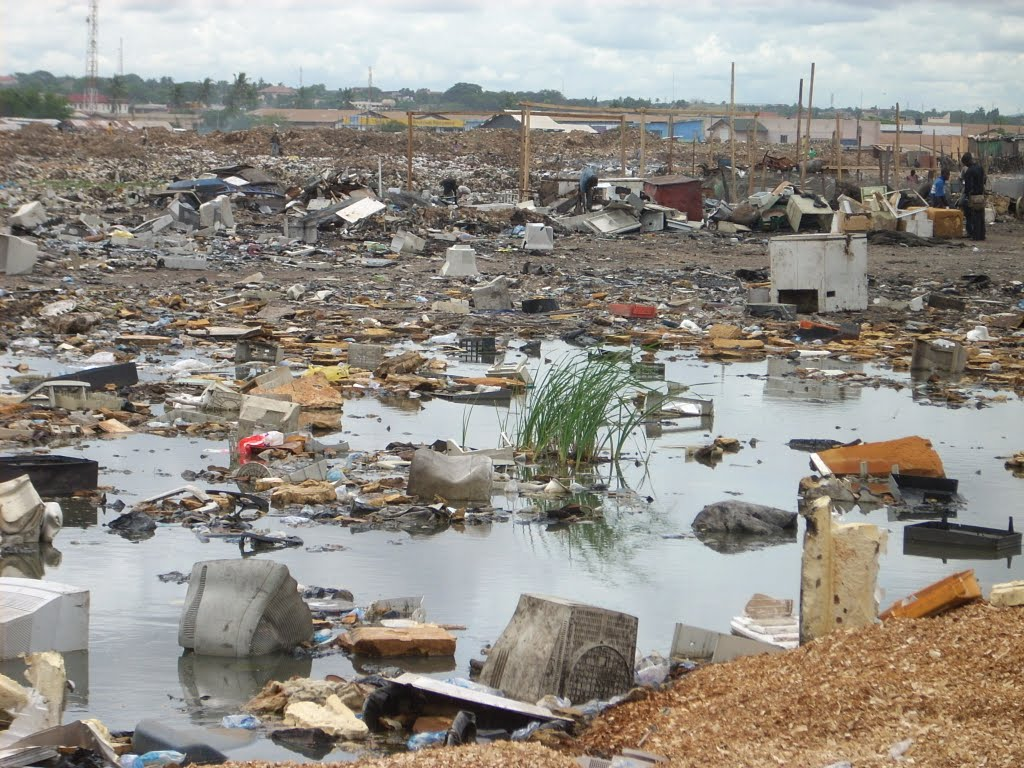
\includegraphics[width=0.5\textwidth]{../inputs/images/ewaste_jack_caravano.jpg}
  \caption{Foto do bairro de Agbogbloshie em Acra. Autorizado por Jack Caravanos, 
           Professor da \textbf{School of Public Health} em \textbf{Hunter College, CUNY}
           Nova Iorque, Estado Unidos da América. \label{fig:ewaste}}
\end{figure}

%%%%
\subsection{Nima}

Nima é um dos bairros mais pobres de Acra. É formada de assentamentos não 
planejados, compostos principalmente de migrantes das partes rurais e 
imigrantes de países vizinhos que buscam oportunidades de empregos na capital. 
Com moradias extremamente improvisadas, carece de sistema tratamento de esgoto, 
fornecimento de água potável e eletricidade. 

É conhecida localmente por uma feira de comidas típicas permanentemente 
instalada na região (\textbf{Nima Market}), que é inclusive visitada por turistas.
Com população de origem de diversas partes de Gana, Nima possui 
alta diversidade cultural e religiosa.

O principal meio de transporte dos trabalhadores de Nima para a zona industrial
e de serviços de Acra é feito por vans. 
Muitas vias não são pavimentadas e a intensa movimentação de veículos causa 
levantamento de poeira do solo.

O carvão e a lenha são bastante empregados como fontes de energia para preparação de 
alimentos. A figura \ref{fig:nima} mostra imagens de áreas de cozimento típicas no bairro.

\begin{figure}[H]
  \begin{subfigure}[b]{0.5\textwidth}
    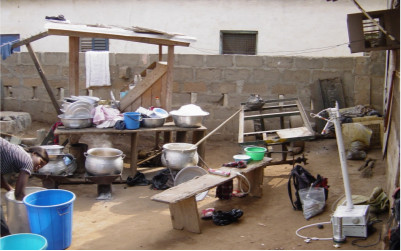
\includegraphics[width=\textwidth]{../inputs/images/zheng/nima1.jpg}
    \caption{}
  \end{subfigure}%
  \begin{subfigure}[b]{0.5\textwidth}
    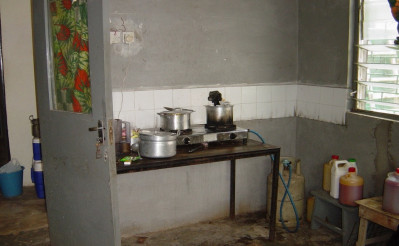
\includegraphics[width=\textwidth]{../inputs/images/zheng/nima2.jpg}
    \caption{}
  \end{subfigure}
  \caption{Fotos de residências de Nima, por Raphael Arku \label{fig:nima}}
\end{figure}

  \section{Poluição do Ar}

Poluição do ar urbana é uma complexa mistura de emissões e naturais e 
antropogenicas.  

O que é material particulado?

Tipos de classificações de Material Particulado: tamanho, por formação 
(primária ou secundária), 
composição química, remoção da atmosfera. (colocar a figura clássica do seinfeld de distribuição), forma da partículas (espérica, espiga, ...) ?

nucleação: condensação de vapores quentes (formando núcleo de condensação) ou durante transformação de gás em partícula. Remoção: aglomeração. 

acumulação: formação: from nucleação através coagulação ou condensação de vapores.remoção: deposição seca ou úmida.

grossas: processos mecânicos: fragmentação, movimentação, manuseio. remoção: sedimentação.

Qual faixa é mais numerosa? usar aquele trabalho do Seinfeld da Fátima?
Qual a composição química por faixa?

fina: íons $SO_4^=$ e $ NO_3^-$, carbono elementar, carbono orgânico, compostos orgânicos elementar condensados?, metais (cádmio, níquel, vanádio, zinco, cromo, ferro, mercúrio), sulfatos, nitratos, nitrato amônia?  
o óxido de nitrogênio (NOx) e amônia NH3 formam  nitrato de amônio e 
o dióxido de enxofre (SO2) amônia NH3 formam o sulfato de amônio, portanto são secundário. 

Qual a diferença da composição entre ambiente rural e urbano.
Artigo que a fátima deu seria interessante... 

grossa: solo, fuligem, pólen. origem mineral: Si, Al, ferro, K, Ca e metais alcalinos.

nomenclatura adotada

relação com sistema respiratório humano (deposição em função do diâmetro da partícula).
as partículas mais finas (PM2.5) chegam nos bronquíolos e as maiores (ainda no PM2.5) só alcançam os alvéolos. e como o corpo as elimina? Macrófago alveolar ou o sistema linfático a expulsam? 
As maiores ficam no nariz (traqueobrônquica) nasofaringe . 
Os vírus são PM2.5 e bactérias são PM10, lega né?

ao depositar em folhas, as partículas impedem a absorção de luz. 


visibilidade

formação de nuvens.

danos a saúde (saldiva e WHO) e ao ambiente.

Legislação nacional e internacional.

fontes naturais e antropogênicas. 
móveis e estacionárias. SPECIATE. As fontes depende da região.


  \section{Objetivos}

O objetivo desta pesquisa é identificar e quantificar 
as fontes de poluição do ar, bairro de Acra,  
Caracterizar o Material Particulado em Acra, capital de Gana, na África.
Aperfeiçoar a metodologia numérica empregada na quantificação de elementos 
químicos e de black carbon, buscando particularmente a determinação mais
consistente das incertezas nos valores medidos.

Para buscar identificar fontes emissoras de PM2,5, e estimar seus impactos, utilizou-se o método estatístico PMF (PAATERO, 1997)


\chapter{Materiais e Métodos}
  %%%%
\section{Amostragem}
%TODO: citar artigo do harvardinho (Impactor Desing)
% http://maps.google.com/maps/ms?ie=UTF8&hl=en&msa=0&msid=116003586198857296821.00046d7e7367b947abe12&z=12

Foram coletadas, entre Novembro de 2006 e Agosto de 2008, 858 amostras válidas, 
de 48 horas, em dois sítios de \textbf{Nima}, sendo um localizado perto da rodovia
(+5° 34' 54.00", -0° 11' 56.30") e outro parte residencial do 
bairro (+5° 35' 2.00", -0° 11' 58.80").

A coleta foi diária, mas houve dias sem coleta devido a falta de eletricade e
filtros danificados no transporte ou na troca no amostrador. 
O tempo de amostragem de 48 horas, foi definido antes da entrada \textbf{USP} 
no projeto e trouxe dificuldades nas análises multivaridas, pois o
ciclo de 48h para a amostragem dificulta a captação das especificidades 
de cada uma das fontes.

As amostras de foram coletadas em filtro de teflon do tipo 
\textbf{PTFE} de 37 $mm$ de diâmetro orifícios de 0,2 $\mu m$ de diâmetro. 

Para $MP_{10}$ utilizou-se impactador Harvard com $D_{50}$ de $10 \mu m$ 
com fluxo de $10,0 L/min$ \citep{marple1987}. 
Nas medidas de $MP_{2,5}$, também utilizou-se impactador Harvard, 
mas com $D_{50}$ de $2,5 \mu m$ acoplado com um \textbf{inlet} 
responsável fazer a filtragem de $MP_{2,5}$.

Filtros brancos de campo e laboratórios foram separados para avaliar 
possíveis contaminações no tranporte e manipulação das amostras. 

O laboratório da \textbf{Harvard School of Public Health} foi
utilizada para pesagem das amostras.
Os filtros foram pesados antes e depois da coleta, usando uma balança 
microanalítica \textbf{(Mettler Toledo MT5)} com precisão de $1 \mu g$, 
seguindo procedimentos padrões de controle de umidade ($39 \pm 2 \%$), 
temperatura ($20,5 \pm 0,2 ^{\circ} C$) e eliminação de cargas eletrostáticas 
(fonte de polônio).
Cada pesagem foi realizada duas vezes e o valor final foi a média das 
duas medidas.

As concentrações foram calculadas a partir dos volumes 
medidos por um integrador de volume.


I confirmed with Jose Vallarino who provided
>>>>certain uncertainty parameters to EPA.
>>>>
>>>>1) 5\% flow rate uncertainty is a standard value used here (HSPH).
>>>>2) 6.7 sq.cm for 37-mm filters with
>>>>uncertainty 0.134 sq.cm is a standard value
>>>>measured in HSPH. However, Jose said the
>>>>sample deposit area uncertainty
>>>>measured/calculated by you might be better since you used an SEM.
>>>>3) We did not provide monitor correction, my
>>>>best guess is they did not use it.
>>>> 

>>  I believe this is a standard number used
>>>>> by EPA. EPA use 10.65 sq.cm
>>>>> for 47-mm filters, 6.7 sq.cm for 37-mm filters.
>>>>>
>>>>>  The filter deposition area uncertainty of
>>>>> 37-mm filters is 0.134 sq.cm. I could confirm this with them 




  %%%%
\newpage
\section{Fluorescência de Raios X}

Para quantificar a composição elementar (10 < Z < 83) das 
amostras foi utilizada a técnica não-destrutiva de Fluorescência de Raios X 
(XRF), um método analítico quali-quantitativo, multielementar, 
que mede os raios X característicos emitidos pelos átomos da amostra, 
depois de também serem excitados por raios X. Permite análise simultânea dos 
elementos químicos e não exige pré-tratamento dos alvos.

Há basicamente três etapas envolvidas na técnica de medida de raios X 
característicos: excitação da amostra, emissão de raios X pelos átomos da amostra
e detecção. A excitação pode ocorrer por feixe de raios X (ou raios gamas) 
produzido em fontes radioativas, por partículas aceleradas 
(elétrons, prótons, alfas etc) ou 
por tubos geradores de raios X quando submetidos a diferença de potencial
\citep{jenkins1988}.

No caso da XRF, a excitação ocorre por um feixe de raios X incidente, que  
expulsa os elétrons das camadas mais internas do átomo (K, L e M) 
produzindo vacâncias. Para tal, a energia do feixe incidente deve ser maior 
que a energia de ligação dos elétrons nessas camadas. Um átomo com vacância é 
instável e rapidamente elétrons das camadas mais externas preenchem as vacâncias,
liberando fotóns e estabilizando o átomo, sendo a energia destes fótons 
correspondentes às energias de transição entre camadas do átomos, 
característica de cada elemento químico. O processo de excitação do átomo 
é ilustrado classicamente na figura \ref{fig:shimadzu_atomo}.

\begin{figure}[H]
  \centering
  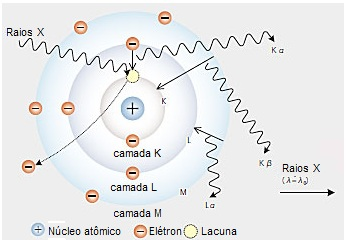
\includegraphics[width=0.5\textwidth]{../inputs/images/shimadzu_atomo.jpg}
  \caption{Ilustração clássica do fenômeno de fluorescência de raios X no átomo. 
           Figura que acompanha o manual da Shimadzu da série de equipamentos
           EDX 700. \label{fig:shimadzu_atomo}}
\end{figure}

As transições dos elétrons entre os níveis quânticos K, L e M encontram-se 
tipicamente na faixa dos raios X, tendendo a ultravioleta (UV) e luz visível,
conforme ocorram em transições atômicas de menor energia no átomo.

Transições da camada L para K são do tipo $K_{\alpha}$, de M para K 
são $K_{\beta}$ e de M para L são $L_{\alpha}$ ou $L_{\beta}$. 
As camadas L e M possuem ainda subníveis de energia, o que resulta em diversas
combinações de transições, sendo algumas delas proibidas, e outras 
com diferenças de energia indistinguíveis para os detectores utilizados 
neste método analítico (XRF-ED).

As principais transições possíveis estão sintetizada na figura \ref{fig:siegbahn}, 
segundo a notação desenvolvida por Siegbahn \citep{jenkins1991}. A referida 
notação, permite identificar melhor os subníveis de origem e destino, por exemplo, 
a transição de $M_{IV}$ para $L_{III}$ é uma transição do tipo $L_{\beta_1}$. 

\begin{figure}[H]
  \centering 
  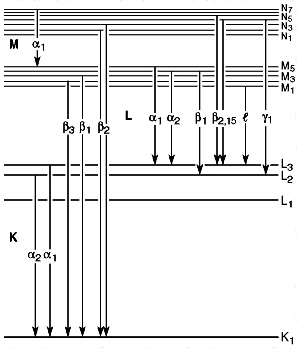
\includegraphics[width=0.5\textwidth]{../inputs/images/Siegbahn.jpg}
  \caption{Transições de elétrons entre os subníveis das camadas K, L e M. 
           Figura extraída de \citet{jenkins1991}. \label{fig:siegbahn}}
\end{figure}

Na prática, dependendo do modo de detecção dos raios X, agrupa-se transições 
dos subníveis e trabalha-se com as denominações de linhas K e L apenas. As linhas
$K_{\alpha}$ são as mais intensas, oferecendo melhor limite de detecção
para um elemento, mas quando muito energéticas, podem ultrapassar a
faixa de sensibilidade do detector empregado. Nestes casos as linhas L passam a 
ser analisadas. No modelo de XRF usado nesta pesquisa, analisou-se as linhas K, 
desde o sódio (Na) até o nióbio (Nb), e as linha L, do molibdênio (Mo) até o chumbo (Pb).  
 
%%%%
\subsection{Tipos de XRF}

Há essencialmente dois tipos principais de equipamentos de XRF que se 
diferenciam pelo modo como os raios X são detectados: fluorescência de raios 
X dispersivo em comprimento de onda (XRF-WD) e fluorescência de raios X 
dispersivo em energia (XRF-ED).

Na XRF-WD os raios X da amostra sofrem difração em um cristal, quantificando-se
os elementos químicos pela contagem de fótons nos ângulo de difração $\theta$, 
característicos dos elementos, segundo a lei de Bragg:

\begin{equation}
	\label{eq:bragg}
	2d sen(\theta) = n \lambda
\end{equation}

Onde, $d$ é 1a distância entre planos do cristal, $\theta$ o ângulo de incidência 
em relação ao plano considerado, $\lambda$ o comprimento de onda 
(e, portanto, a energia) da radiação incidente e $n$ um inteiro.
Esse tipo de equipamento permite uma grande resolução dos comprimentos de onda 
(energia) característicos dos elementos, facilitando detectá-los e, geralmente, 
com bom limite de detecção (LD).
Entretanto, apresentam diversos problemas práticos quando empregados em filtros 
de aerossol atmosférico. Em função disso há uma preferência pelos sistemas 
dispersivos em energia nesse campo de análise. 

A XRF-ED usa detectores de semicondutores capazes de discriminar energias 
próximas com alta resolução temporal, viabilizando a detecção simultânea dos 
elementos químicos através da amplitude do pulso eletrônico produzido no 
detector, proporcional à energia do fóton incidente. O sistema eletrônico do 
equipamento faz a conversão analógica-digital da intensidade do pulso, 
acumulando a contagem por energia em um multicanal. O detector mais empregado é 
o de silício ativado com lítio Si(Li). 

Neste sistema, o LD das análises é particularmente limitado pelos raios X de 
excitação que sofrem reflexão na amostra e também chegam ao detector. 
Formam assim uma contagem de fundo (\textit{background}) que concorre com 
aquela proveniente dos picos característicos. 
Fluorescência de raios X polarizada (XRF-EDP) e fluorescência de raios X por 
reflexão total (XRF-T) são dois sistemas que têm sido empregados 
para reduzir o \textit{background} e melhorar significativamente o LD.

Na XRF-EDP, excita-se a amostra com raios X polarizados e se ajusta o ângulo 
de detecção a 90 $\degree$ deste feixe \citep{dzubay1974}. Nesta direção a 
reflexão do feixe incidente polarizado é pequena, obtendo-se grande redução 
na intensidade do fundo e, consequentemente, no LD, tipicamente de fator 2 a 10
dependendo do elemento e das condições de irradiação comparadas 
\citep{meel2009}.

A XRF-T emprega a propriedade da radiação eletromagnética incidente abaixo do
ângulo crítico sobre uma superfície. Incidindo-se um feixe que resvale a amostra
com um ângulo bem pequeno, este excitará uma fina camada da superfície, 
penetrando muito pouco no suporte. Desta forma um detector posicionado 
perpendicularmente à superfície receberá muitos fótons característicos gerados 
pela amostra e pouco fundo refletido no suporte, melhorando o LD
\citep{yoneda1971} e \citep{aiginger1974}.

%%%%
\subsection{Características da XRF-ED utilizada}

Neste trabalho foi utilizado uma XRF-ED da marca Shimadzu modelo EDX 720HS, 
apresentado na figura \ref{fig:xrfed_iag},
pertencente ao Laboratório de Poluição Atmosférica Experimental (LAPAE) 
da Faculade de Medicina da USP e instalado no LAPAt. 

\begin{figure}[H]
  \centering
  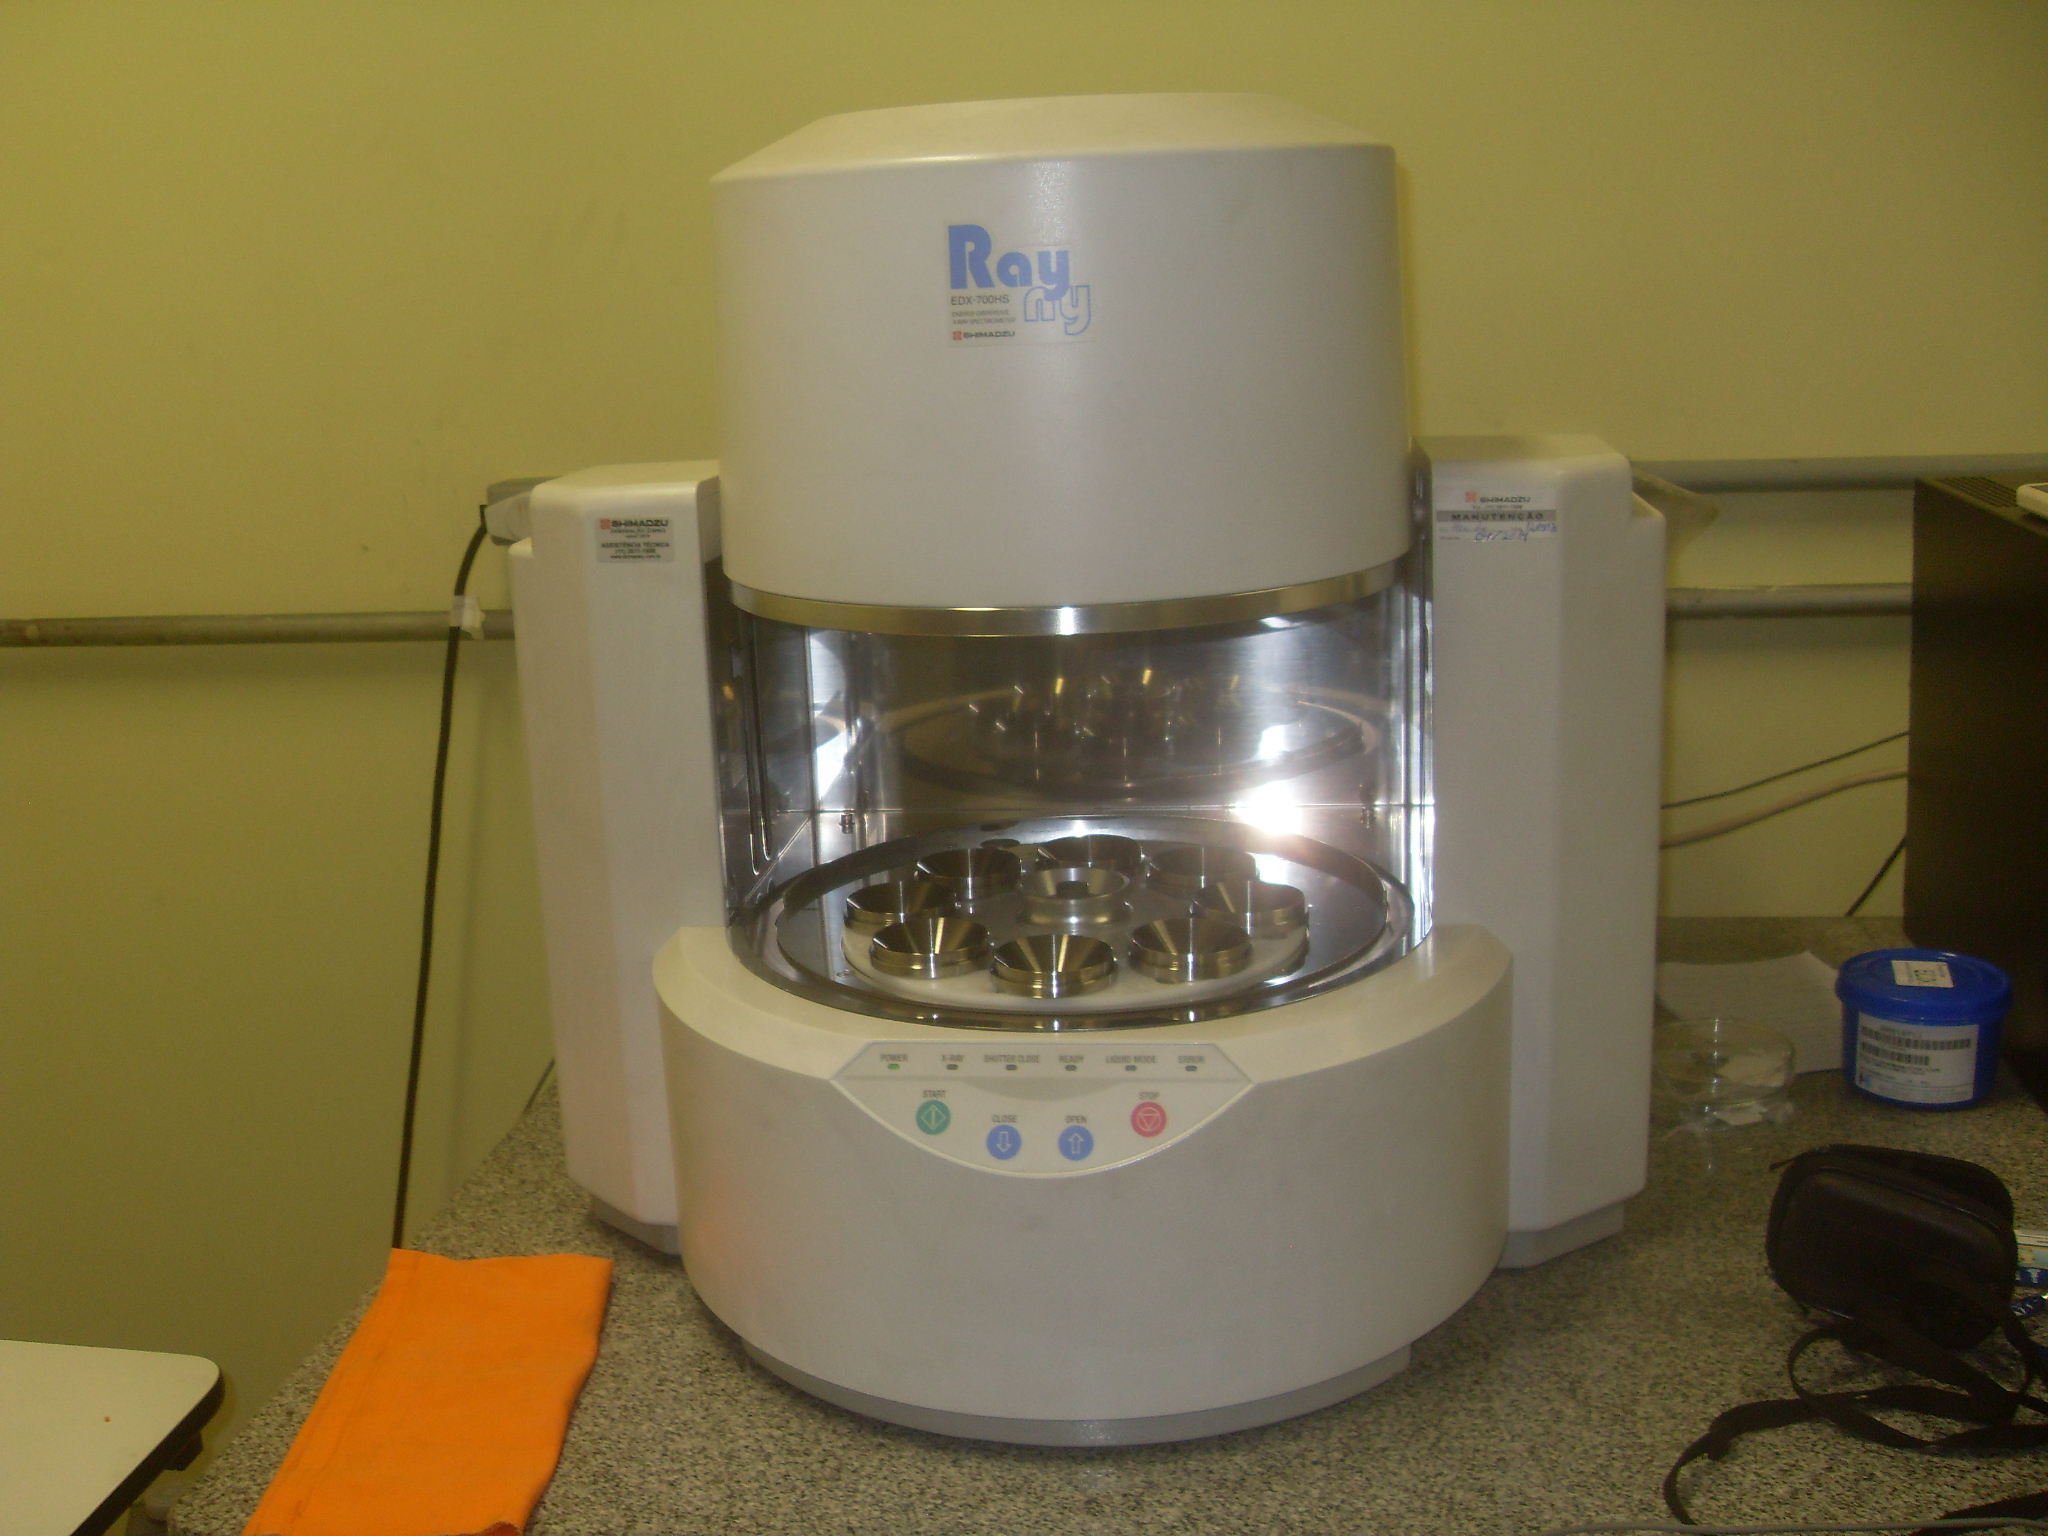
\includegraphics[width=0.5\textwidth]{../inputs/images/xrf-ed-IAG-USP.jpg}
  \caption{XRF-ED Shimadzu modelo EDX 720HS - LAPAt. \label{fig:xrfed_iag}}
\end{figure}

Um tubo de ródio (Rh) submetido a uma diferença de potencial 
de 50 kV foi utilizado para geração do feixe de raios X.
O detector de silício ativado com lítio Si(Li) possui sensibilidade
para medida de fótons com energia entre 1 e 20 keV acoplado a um sistema 
eletrônico com multicanal de 2048 canais capaz de quantificar simultaneamente 
os elementos desde o Na até o Pb. Para remoção da radiação da linha L do feixe 
de raios X do tubo de ródio, de energia próxima de 2,6 keV, um filtro de 
alumínio foi posto entre o feixe e a amostra, melhorando o limite de detecção 
dos elementos com energia igual ou menor que 2,6 keV. O diâmetro do feixe de 
raios X é definido por um colimador de 10 mm, garantindo a irradiação de uma 
área representativa e homogênea da amostra. 

O tempo vivo de irradiação de cada amostra foi $\pm$ 960 minutos, ajustando-se 
a corrente para manter o tempo morto em 20\%. Desejava-se desta forma fixar a 
taxa de contagem, obtendo-se ao final o mesmo número total de fótons contados 
em cada espectro. Esse mecanismo permite melhorar o LD dos elementos presentes 
em amostras menos carregadas. Isso nem sempre foi possível já que a corrente 
máxima no tubo gerador de raios X era de 1000 $\mu A$. 

A figura \ref{fig:xrfed_software} foi extraída do software que acompanha o 
equipamento da Shimadzu e permite verificar em tempo real características
da análise como a voltagem e corrente no tubo, presença e tipo de filtro, 
informação sobre o vácuo na câmera, dentre outros dados que ajudam no 
acompanhamento da análise. 

\begin{figure}[H]
  \centering
  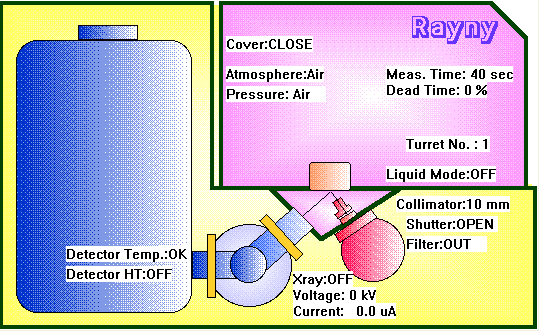
\includegraphics[scale=0.4]{../inputs/images/edx_iag_monitor.png}
  \caption{Software da XRF-ED Shimadzu 720HS, tela de verificação 
           do estado do equipamento. \label{fig:xrfed_software}}
\end{figure}

O EDX 720HS permite análise automática de amostras encaixadas em carrosséis 
de 8 ou 16 posições. O LAPAt contava então apenas com o carrossel de 16 
posições. Foi necessário adquirir um com 8 posições, cujos receptáculos admitiam
o maior diâmetro dos filtros de PTFE, que não podem ser cortados e remontados 
como os de policarbonatos (figura \ref{fig:carrossel8}).

\begin{figure}[H]
  \centering
  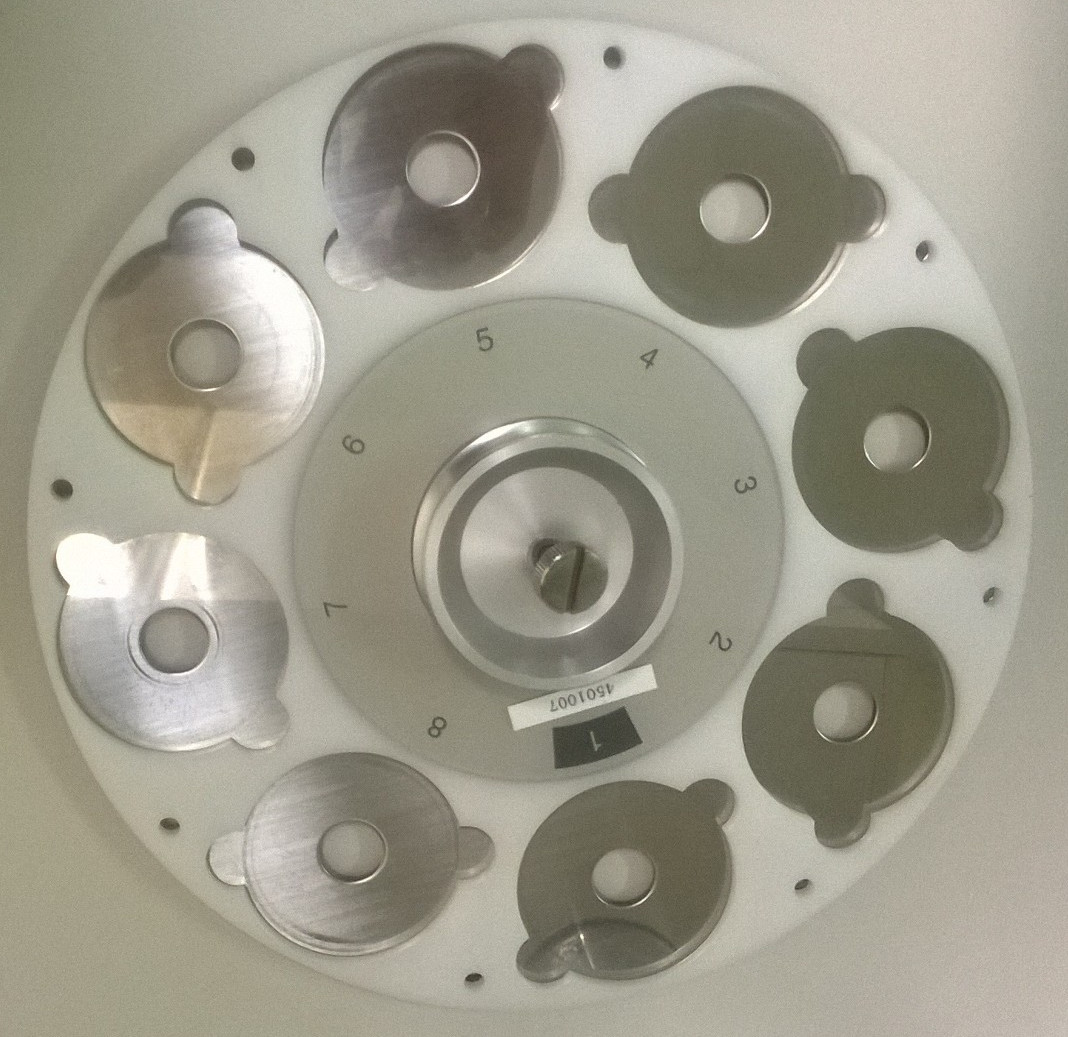
\includegraphics[width=0.5\textwidth]{../inputs/images/carrossel8.jpg}
  \caption{Carrossel de 8 posições adquirido para XRF-ED Shimadzu 720HS. 
           \label{fig:carrossel8}}
\end{figure}

Para eliminar as ondulações típicas que ocorrem nos filtros de PTFE, 
projetou-se um suporte de aço inox que comprimia sua moldura, mantendo plana 
a superfície a ser analisada. Ao mesmo tempo, o peso deste suporte impedia que 
o filtro voasse quando era feito ou quebrado o vácuo na câmera 
(figura \ref{fig:suporte8}).

\begin{figure}[H]
  \centering
  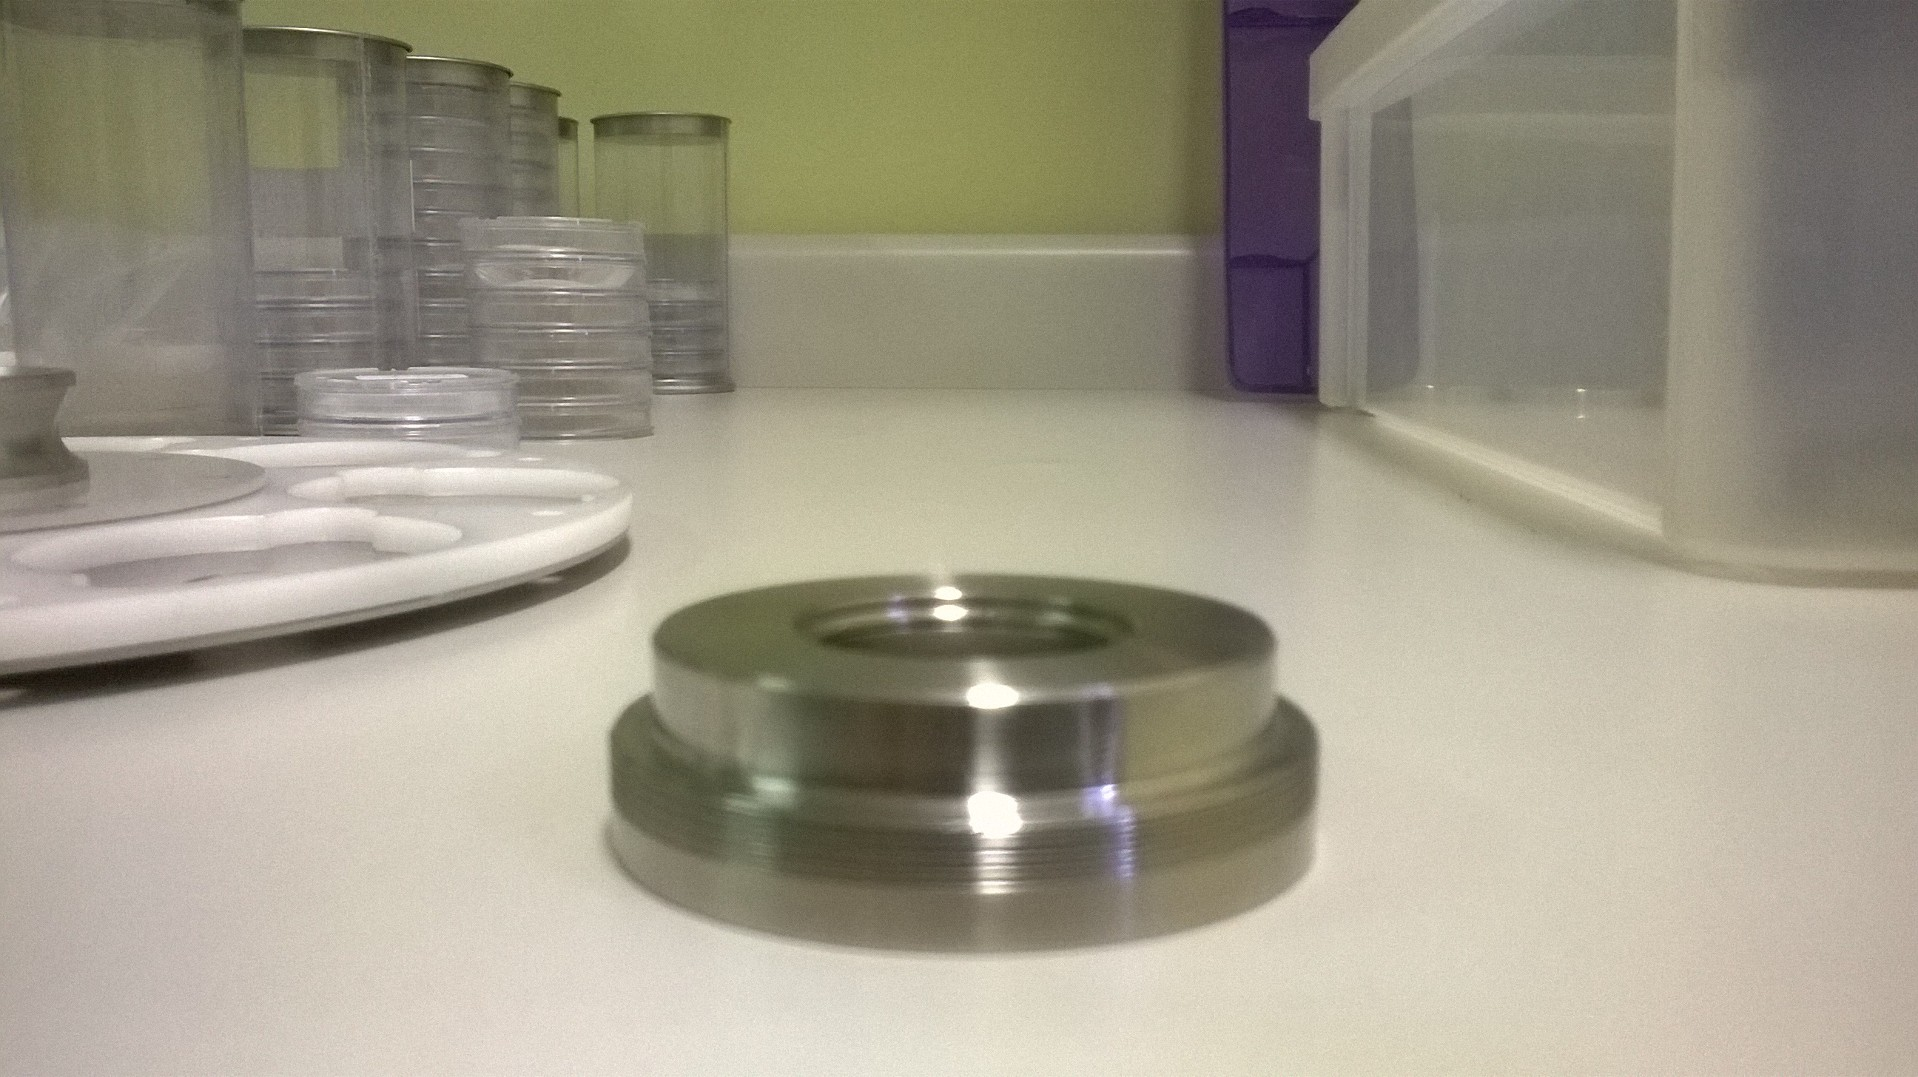
\includegraphics[width=0.5\textwidth]{../inputs/images/suporte8.jpg}
  \caption{Suporte para filtros de PTFE, projetado no LAPAt para carrossel de 
           8 posições e produzido pela oficina da FAP no 
           Instituto de Física da USP. \label{fig:suporte8}}
\end{figure}

%%%%
\subsection{Calibração do XRF-ED}

A massa por unidade de área, depositada sobre os filtros tipicamente usados em 
pesquisas de aerossol atmosférico, permite tratá-los como amostras finas,
ou seja, o efeito de matriz, interações dos raios X característicos com os 
elementos das amostras causando absorção ou reforço do número de fótons de 
raios X característicos, são pequenos diante da precisão do método,
podendo desconsiderá-lo. Nesta aproximação, pode-se relacionar de modo 
simples o número de fótons contados sob o pico característico de um elemento, 
presente no espectro obtido, com a sua massa na amostra irradiada:

\begin{equation}
  \label{eq:contagem}
  N(Z) = R(Z) \cdot I \cdot \Delta t  \cdot \frac{m(Z)}{A}
\end{equation}

Onde R(Z) é chamado de fator de resposta, I é a corrente de excitação do tubo 
de raios X, determinando, portanto, o fluxo de raios X que chegam à amostra, 
$\Delta t$ é o tempo vivo de irradiação e m(Z)/A é a densidade superficial
(massa por unidade de área) dos elementos Z presentes na amostra. 
Pressupõe-se distribuição uniforme da massa na superfície do filtro.

O termo R(Z) depende da seção de choque de cada elemento com o feixe de 
raios X incidente (incluindo modificações por eventuais filtros moduladores 
de suas características), da curva de eficiência do detector de raios X, 
da eficiência de operação do tubo de raios X e da geometria do sistema, 
incluindo os diâmetros de colimadores selecionados. Mantendo estes parâmetros 
fixos e irradiando alvos padrões com densidades (d(Z) = m(Z)/A) 
conhecidas, pode-se calcular R(Z):

\begin{equation}
  \label{eq:fator_de_resposta}
  R(Z) = \frac{N(Z)}{d(Z) \cdot I \Delta t}
\end{equation}

Considerando que a incerteza da corrente e do tempo vivo são desprezíveis 
perto da incerteza da densidade e da contagem, a incerteza no fator de resposta
pode ser calculada por propagação de erro destas variáveis:

\begin{equation}
  \label{eq:erro_fator_de_resposta}
  \sigma_{R(Z)}^2 = {R(Z)}^2 \cdot \left( \left(\frac{\sigma_{N(Z)}}{N(Z)}\right)^2 + 
                                      \left(\frac{\sigma_{d(Z)}}{d(Z)}\right)^2 
                                   \right)
\end{equation}

Dados ambientais são reportados em medidas de concentração ($\mu g/m^3$),
razão da massa m(Z) pelo volume amostrado. Conhecendo o fator de resposta 
R(Z) pode-se calcular a massa m(Z) depositada na amostra, usando a equação 
\ref{eq:contagem}, tomando como valor da área A aquela da deposição de aerossol
no filtro:

\begin{equation}
  \label{eq:xrfedmassa}
  m(Z) = \frac{N(Z) \cdot A}{ R(Z) \cdot I \cdot \Delta t}
\end{equation}

Empregando novamente a expressão da propagação de erro para variáveis 
independentes, a incerteza na massa será:

\begin{equation}
  \label{eq:erro_massa}
  \sigma_{m(Z)}^2 = {m(Z)}^2 \left( \left(\frac{\sigma_{N(Z)}}{N(Z)}\right)^2 + 
                                  \left(\frac{\sigma_A}{A}\right)^2 + 
                                  \left(\frac{\sigma_{R(Z)}}{R(Z)}\right)^2 
                             \right)
\end{equation}


Vê-se, entretanto, que para cada espécie química de interesse, seria necessário
ao menos um alvo de calibração para calcular seu R(Z). Alvos padrões finos, 
com densidade elementar conhecida, podem ser comprados ou produzidos, dependendo
da precisão desejada. Neste projeto foram adquiridos alvos padrões da 
Micromatter, com incerteza nominal de 5\%. Mas esta empresa não produz alvos 
com proporção estequiométrica quantificada para todas espécies químicas.
Assim, trouxemos para a XRF-ED o conceito proposto por \citet{tabacniks2000}
implementado no sistema PIXE (Particle Induced X-Ray Emission) do IFUSP que permite obter uma 
calibração abrangendo elementos de número atômico no intervalo 10 < Z < 83. 
 
Adotou-se, ainda, uma metodologia estatística robusta para estimativa das 
incertezas da calibração usando MQM. Essa preocupação em definir 
adequadamente as incertezas deve-se, particularmente, ao fato de que elas 
ponderam o peso das variáveis na modelagem por PMF.

Como exemplo para conhecer o forma da curva de calibração, o gráfico da figura 
\ref{fg:edxrfcalib} apresenta os R(Z) dos alvos padrões da Micromatter 
irradiados em maio de 2010. 

\begin{figure}[H]
  \begin{subfigure}[b]{0.45\textwidth}
    \includegraphics[width=\textwidth]{../outputs/plot_R_maio2010K.pdf}
    \caption{linha K}
  \end{subfigure}%
  \begin{subfigure}[b]{0.45\textwidth}
    \includegraphics[width=\textwidth]{../outputs/plot_R_maio2010L.pdf}
    \caption{linha L}
  \end{subfigure}
  \caption{Fatores de respostas, R(Z), para alvos padrões da 
           Micromatter irradiados em maio de 2010. 
           \label{fg:edxrfcalib}}
\end{figure}

Nota-se que é possível fazer um ajuste polinomial sobre esses dados, 
o que tanto melhora a precisão para todos os R(Z), quanto fornece seu valor
para elementos que não possuem alvos padrões. O fator de resposta reflete 
o arranjo experimental, mudanças físicas
nesse arranjo alteram o valor de R(Z), assim como a progressiva fadiga do detector
ou do tubo. Portanto, a calibração deve ser realizada periodicamente.

%%%%
\subsection{Incertezas dos ajustes com Mínimos Quadrados Matricial}

As incertezas dos ajustes polinomiais das calibrações do XRF-ED e da 
intercalibração de TOT e refletância de BC foram estimadas com o método 
Mínimos Quadrados Matricial (MQM) desenvolvida por \citet{helene2006}
e parcialmente reproduzida a seguir (com adaptações).

Dadas as variáveis $Y_i$ e $X_i$ relacionadas polinomialmente:

\begin{equation}
  \label{eq:polinomio}
  \begin{split}
    y_1 = a + b x_1 + c{x_1}^2 + d{x_1}^3 + ...\\
    y_2 = a + b x_2 + c{x_2}^2 + d{x_2}^3 + ... \\
    ...
  \end{split}
\end{equation}

ou na forma matricial:

\begin{equation}
  \label{eq:polinomioMatriz}
  [Y] = [A][X]
\end{equation}

Os coeficientes ajustados [Ã] são dados por:

\begin{equation}
  \label{eq:coeficientesajustados}
  [Ã] = [V_{Ã}] ([X]^T {[V_Y]}^{-1} [Y])
\end{equation}

Sendo $[V_{Ã}]$ a matriz de covariância dos coeficientes, dada por:

\begin{equation}
  \label{eq:matrizcovariancia}
  [V_{Ã}] = ([X]^T [V_Y]^{-1} [X])^{-1}
\end{equation}

A partir dos coeficientes ajustados [Ã] na equação \ref{eq:coeficientesajustados},
pode-se calcular os $[\tilde{Y}]$ ajustados,

\begin{equation}
  \label{eq:polinomioajustado}
  [\tilde{Y}] = [Ã][X]
\end{equation}

A diagonal da matriz de covariância de $[\tilde{Y}]$, $[V_{\tilde{Y}}]$, 
representa a incerteza dos valores ajustados:

\begin{equation}
  \label{eq:matrizcovarianciaY}
  [V_{\tilde{Y}}] = [X] [V_{Ã}]^{-1} [X]^{-1}
\end{equation}

No caso da XRF-ED, quando se calcula R(Z) apenas a partir do alvo de 
calibração do elemento Z, é a incerteza de produção deste alvo que determina 
a precisão de R(Z). Mas com o procedimento de ajuste por MQM, sob os 
R(Z) disponíveis, é o conjunto destes valores e de suas incertezas, bem como a 
qualidade do ajuste que determinam a incerteza ajustada, oferecendo uma 
melhora significativa na precisão e na exatidão dos R(Z).

%%%%
\subsection{Fontes de erro no branco}

A massa depositada no filtro amostrado $m(Z)_{medido}$ para um certo elemento Z
é composta pela massa coletada na amostragem m(Z) mais a massa do filtro 
branco $m_{B}(Z)$.

Um conjunto de 10 amostras brancas (entre campo e laboratório) foram analisadas, 
para eliminação da contaminação dos próprios filtros, assim como de 
transporte e manipulação.

A seguir, a equação \ref{eq:contagem} está escrita para representar o número de contagens de alvos amostrados, isto é, com sobreposição da massa coletada na amostragem $m(Z)$ e a massa do branco $m_B(Z)$: 

\begin{equation}
  \label{eq:contagem_medida}
  N(Z)_{medido} = R(Z) \cdot I \cdot \Delta t \cdot \left( \frac{m(Z)}{A} + \frac{m_B(Z)}{A} \right)
\end{equation}  

Quando as amostras brancas são irradiadas separadamente, o número de contagens é dado por:

\begin{equation}
  \label{eq:contagembranco}
  N_B(Z) = R(Z) \cdot I_B \cdot \Delta t_B \cdot \frac{m_B(Z)}{A}
\end{equation}

Isolando-se $m_B(Z)$ em \ref{eq:contagembranco} e substituindo em 
\ref{eq:contagem_medida}, encontramos o número de contagens corrigido nos alvos amostrados
(isto é, excluindo a contaminação das amostras brancas):
 
\begin{equation}
  \label{eq:contagemcorrigida}
  N(Z) = N(Z)_{medido} - I \cdot \Delta t \cdot \left( \frac{N_B}{I_B \cdot \Delta t_B}  \right)
\end{equation}

A incerteza da contagem corrigida (equação \ref{eq:contagemcorrigida}) é dada por:

\begin{equation}
  \label{eq:erro_contagemcorrigida}
  \sigma_{N(Z)}^2 = \sigma_{N(Z)_{medido}}^2 + \left( \frac{I \cdot \Delta t}{I_B \cdot \Delta t_B} \right)^2 \cdot \sigma_{N_B}^2
\end{equation}

Calcula-se a razão $N_B/(I_B \cdot \Delta t_B)$ para um conjunto de alvos brancos para 
posterior inserção na equação \ref{eq:contagemcorrigida}.

Foi criado colaborativamente por pesquisadores do LAPAt um programa 
em linguagem C que automatiza o cálculo teórico de concentrações apresentado, 
com as devidas correções de branco e propagações de incertezas \footnote{
O código está disponível no repositório de versionamento git da USP 
e pode ser acessado pelo endereço: 
\url{https://git.uspdigital.usp.br/5385361/xrfdensid}}.

%%%%
\subsection{Integração dos espectros}

Realizou-se a integração de todos os espectros obtidos na XRF-ED no
Quantitative X-Ray Analysis System for Windows (WinQxas),
programa desenvolvido para integração numérica de espectros sob o patrocínio 
da Agência Internacional de Energia Atômica (IAEA) \citep{capote2000}.

Obtém-se os parâmetros iniciais da relação linear entre canal e energia,
conhecendo-se ao menos dois picos no espectro, normalmente Ferro e Cálcio, 
no caso de poluição do ar ambiental. 

Os parâmetros iniciais entre a largura do pico à meia altura (FWHM)
dependem da energia (E), do nível geral de ruído (NOISE) no espectro 
e do FANO, dado pela relação: 

\begin{equation}
  \label{eq:fwhm}
   {FWHM}^2 = {NOISE}^2 + 2,35 \cdot FANO  \cdot E
\end{equation}

Os parâmetros iniciais foram determinados a partir de espectros com picos 
bem definidos, como o Ferro, que teve largura à meia altura (FWHM) para 
$K\alpha$ de 138,32 eV ou o Cálcio com 129,14 eV.

Na figura \ref{fig:winqxas} há dois exemplos de espectros abertos no WinQxas
para amostras de Nima, sendo um de uma amostra branca e a outra carregada. Os picos 
característicos de elementos químicos encontrados estão indicados na figura.

\begin{figure}[H]
  \centering
  \begin{subfigure}[b]{0.7\textwidth}
    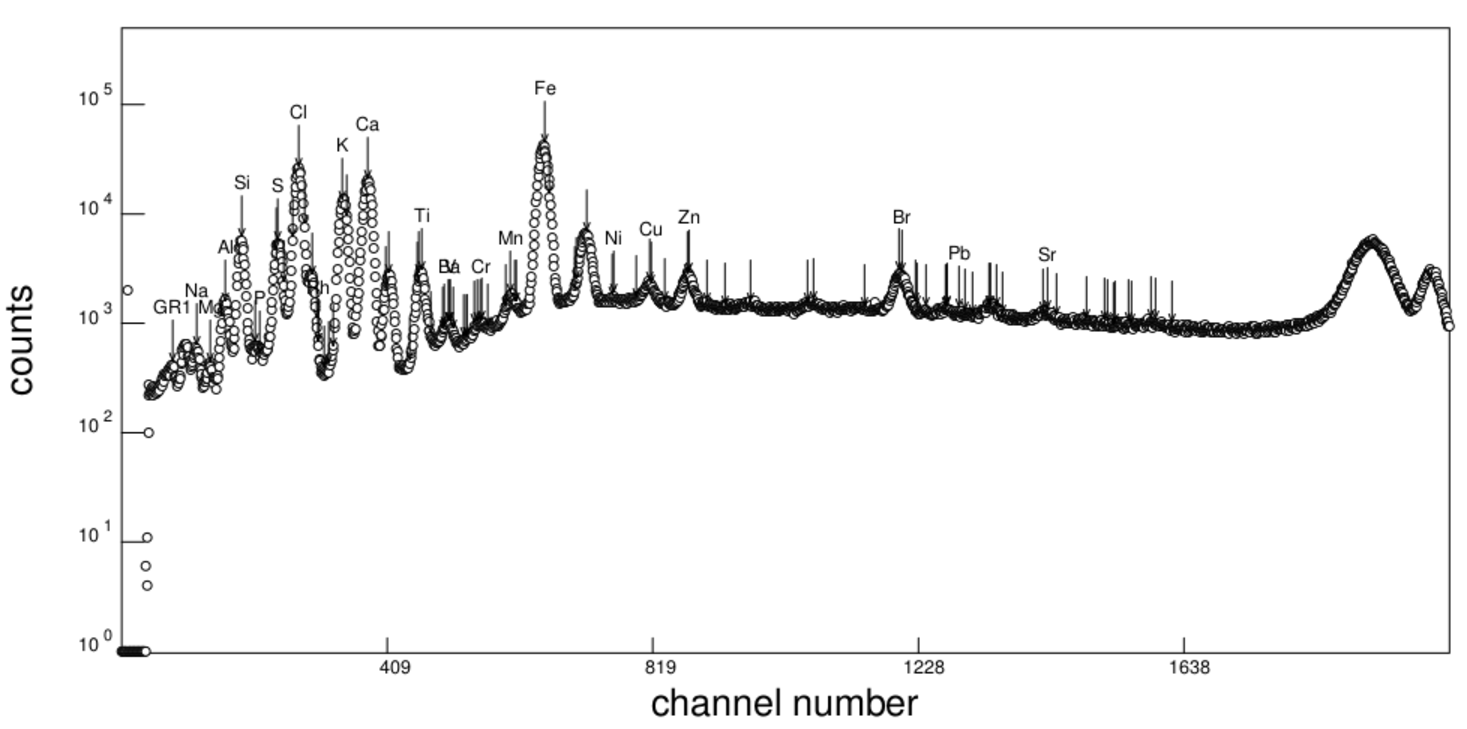
\includegraphics[width=\textwidth]{../inputs/images/winqxas/GHA41editado.pdf}
    \caption{Espectro de amostra carregada (GHA41) - Acra Nima}
  \end{subfigure}
  \begin{subfigure}[b]{0.7\textwidth}
    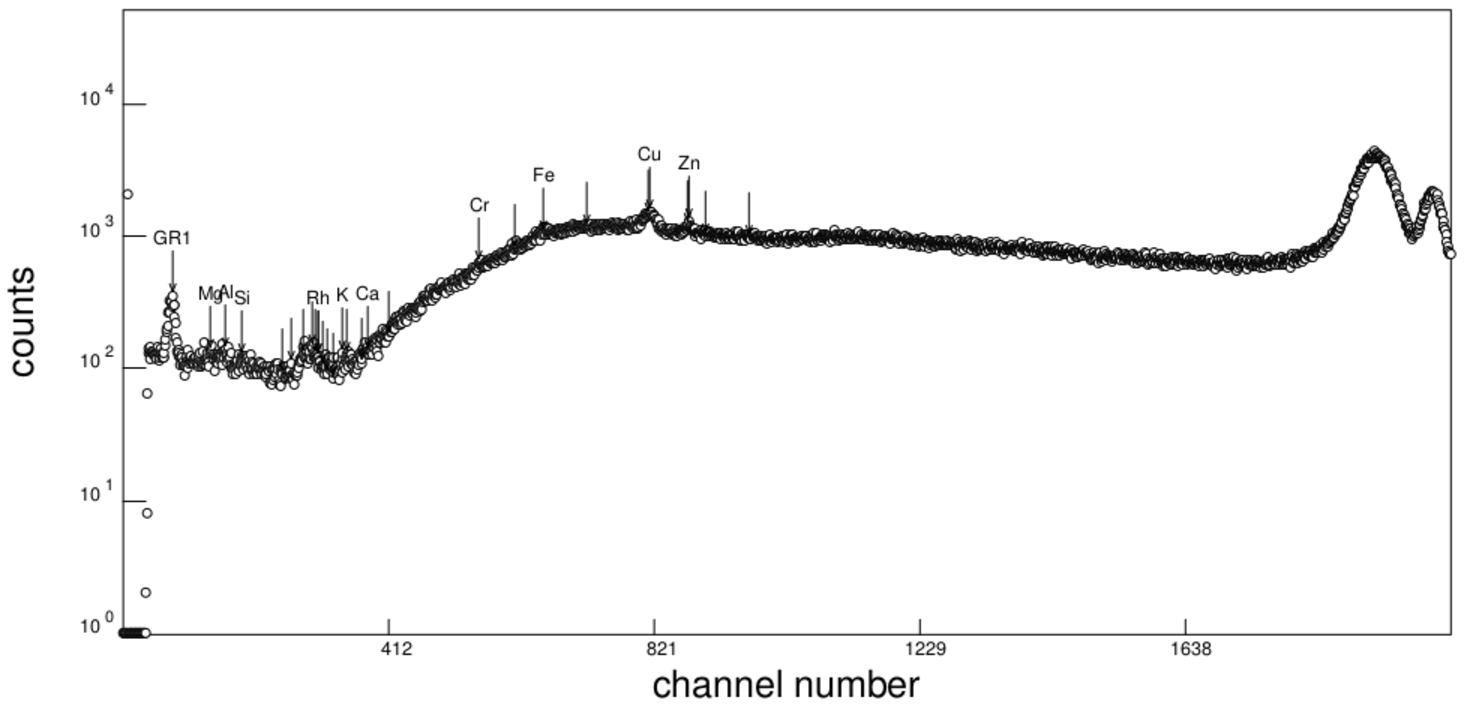
\includegraphics[width=\textwidth]{../inputs/images/winqxas/GPE770editado.pdf}
     \caption{Espectro de amostra branca (GPE770)- Acra Nima}
  \end{subfigure}
  \caption{Espectros para amostra branca e carregada de Nima. \label{fig:winqxas}}
\end{figure}

Na integração dos espectros, pico a pico, deve-se ter atenção 
para identificação e correção dos seguintes eventos em picos com 
muitas contagens: 

\begin{itemize}
  \begin{spacing}{1.0}
  \item pico soma: quando fótons de diferentes elementos são contados
        juntos pelo detector. 
  \item pico escape: quando o fóton incidente excita o silício do detector
        e é contado com energia menor, pois parte foi perdida na excitação 
        do silício. 
  \end{spacing}
\end{itemize}

A seguir, apresenta-se a calibração do multicanal, ajuste linear entre canal 
e energia encontrado a partir do Fe e Ca:

\begin{equation}
  E = 0,0101 \cdot Canal - 0,1335 (keV)
\end{equation}

%%%%
\subsection{Limite de detecção}

O limite de detecção (LD) é a intensidade mínima do pico de um elemento para haver 
detecção da espécie se considerando o tipo de filtro e XRF-ED empregados. 
Irradiando uma amostra branca, obtém-se o número de contagens 
medidas ($N_{fundo}$) sob o pico (fundo do espectro) de cada um dos elementos
medidos.
As contagens de fundo do espectro seguem uma distribuição de Poisson e portanto 
a incerteza para o valor de N contagens é $\sqrt{N}$.
Desta forma, adota-se como LD para um elemento, a condição de que as contagens de seu pico 
característico seja pelo menos três vezes a incerteza na contagem de fundo:

\begin{equation}
  \label{eq:limitedeteccao}
  N_{LD} = 3 \cdot \sqrt{N_{fundo}}
\end{equation}

Pode-se calcular o LD em termos da massa elementar com a 
equação \ref{eq:xrfedmassa}. O limite de detecção muda conforme a quantidade de 
material coletado, sendo maior em amostras carregadas, devido à sobreposição de 
picos e a maior reflexão do feixe na amostra.

Assim, o ideal é calcular o LD em cada amostra, mas ele deve situar-se entre 
aquele medido em um filtro branco e uma amostra com bastante carga.
Os LDs encontrados para os dois tipos de amostras estão apresentados 
nos gráficos da figura \ref{table:ld} em termos de concentrações típicas 
($\mu g / m^3$) para o volume médio de 13,9 $m^3$. 
Note-se que na linha K o LD é alto para elementos de baixo número atômico, 
dificultando a detecção desses elementos, mas melhora com o aumento de Z. 

\begin{figure}[H]
  \begin{subfigure}[b]{0.5\textwidth}
    \includegraphics[width=\textwidth]{../outputs/limitDetectionK.pdf}
    \caption{linha K}
  \end{subfigure}%
  \begin{subfigure}[b]{0.5\textwidth}
    \includegraphics[width=\textwidth]{../outputs/limitDetectionL.pdf}
    \caption{linha L}
  \end{subfigure}
  \caption{Limite de detecção para XRF-ED em termos de concentrações típicas 
           para amostra branca e carregada.
           \label{table:ld}}
\end{figure}

\newpage
\begin{table}[H]
  \centering
  \input{../outputs/LD.tex}
  \caption{Limite de detecção para XRF-ED em termos de concentrações típicas 
           para amostra branca e carregada. \label{table:LD}}
\end{table}

  %%%%
\section{Black Carbon}

Medidas de BC pela técnica de refletância apresentam a vantagem de poderem ser 
realizadas sobre os mesmos filtros empregados para análises gravimétricas, 
XRF ou mesmo em técnicas destrutivas que posteriormente possam vir a ser 
realizadas sobre eles, como cromatografia iônica ou espectroscopia de massa. 
Isso promove a redução das incertezas provenientes de análises que pedem 
diferentes amostradores coletados em paralelo. Também pode diminuir 
significativamente a dimensão da instrumentação em uma pesquisa. Entretanto, 
a refletância é uma medida indireta, cujo resultado depende das características 
do aerossol amostrado. Utilizando o método absoluto TOT para algumas amostras, 
foi possível intercalibrar as medidas de refletância com esse método absoluto, 
permitindo a quantificação do BC nas demais amostras.

%%%%
\subsection{Calibração da refletância usando BC Monarch 71}

Alvos padrões produzidos no laboratório do antigo GEPA-IFUSP (Grupo de Estudos 
de Poluição do Ar), hoje Laboratório de Física Atmosférica (LFA-IFUSP), 
com concentrações conhecidas do BC de referência Monarch 71 (M71) 
\citep{clarke1986}, foram usados por décadas em equipamentos de refletância 
alocados nestes laboratórios e no LAPAt, para a calibração de refletância versus
densidade superficial de BC em filtros que coletaram aerossol atmosférico.

A tabela \ref{table:monarch71} mostra um conjunto de valores medidos em 2007 
para estes padrões (com respectivas médias e incertezas), sobre os quais foi 
feita uma calibração no Lapat, seguindo exatamente os mesmos procedimentos do 
GEPA/LFA-IFUSP. Os novos parâmetros então ajustados ofereciam resultados 
apenas 2,3\% menores que a calibração anterior (1994), do GEPA/LFA-IFUSP. 
Isso revela equipamentos uniformes e grande estabilidade destes padrões. 
Entretanto, essa sistemática de calibração padecia de três problemas.

O primeiro deles refere-se à estreita faixa de valores oferecidas por estes 
padrões que, como pode ser visto na referida tabela, variam entre 30\% e 85\%, 
não cobrindo a região acima de 85\% ou abaixo de 30\%, esta última onde 
posicionam-se os filtros carregados que encontramos no experimento de Gana. 
Mesmo assim, se fosse considerada a linearidade que predomina na relação 
entre densidade de BC e log da refletância, equação \ref{m/a_2}, e acrescida 
no ajuste a massa zero, para qual a refletância é 100\% ($log_{10}$100 = 2), 
poder-se-ia estender o ajuste para uma faixa apreciável de valores.
Mas a função adotada para os ajustes foi uma parábola. Esse foi um segundo 
problema para esta calibração, como se pode verificar na figura 
\ref{fig:monarch71}, essa função distancia-se bastante de um ajuste linear 
conforme nos deslocamos em direção a $log_{10}$ 10, ponto em que a relação da 
massa com o log da refletância começa a perder a linearidade. O gráfico da 
figura \ref{fig:razaoTOTM71} mostra que a margem de erro em alvos carregados 
cresce com o ajuste de 2$\degree$ grau, quando confrontado com a calibração 
baseada em TOT, para filtros coletados em Gana. Note-se, entretanto, que na 
zona de refletância onde havia alvos padrões, as diferenças com o método 
absoluto, por óbvio, são semelhantes. 

A calibração do refletômetro do LAPAt para 2007 usando alvos padrões M71 com 
ajuste de primeiro grau está no gráfico da figura \ref{fig:monarch71}, com 
respectivos dados apresentados na tabela \ref{table:monarch71}.

\begin{figure}[H]
  \centering
  \includegraphics[width=0.5\textwidth]{../outputs/BC_monarch71.pdf}
  \caption{Calibração do refletômetro do LAPAt em 2007 usando alvos padrões M71.
         \label{fig:monarch71}}
\end{figure}

\newpage
\begin{table}[H]
  \centering
  \small
    \input{../outputs/BC_monarch71.tex}
    \caption{Calibração do refletômetro do LAPAt em 2007 usando alvos padrões 
             M71. \label{table:monarch71}}
\end{table}

Procuramos construir uma calibração mais consistente, produzindo alvos de 
calibração que cobrissem toda a faixa de valores entre 0 a 100\% de refletância. 
Mas não encontramos mais o BC M71 para comercializar, assim usamos o BC de 
referência (ASTM-N762) do IPT com o qual produzimos 27 padrões depositados em 
filtros de policarbonato (nuclepore fino de 37 mm, orifícios de 0,4 $\mu m$) 
usando amostrador dicotômico (diâmetro de corte em 2,5 $\mu m$) na câmara de 
ressuspensão do laboratórios da Divisão de Qualidade do Ar da CETESB.

Os valores de refletância nesses filtros variaram de 3,1\% até 98,7\%, mais um 
"zero" de massa teórico com refletância 100\%. As massas foram medidas em 
microbalança analítica $\pm$ 1 g. A figura \ref{fig:bc_cetesb} mostra o ajuste 
entre massa de BC depositada versus o log da refletância medida. Pode-se ver 
que o ajuste linear foi excelente,
indicando que a calibração deve perder linearidade apenas em refletâncias 
inferiores a 5\%.

\newpage
\begin{table}[H]
	\centering
	\small
	\input{../outputs/cetesb2012.tex}
	\caption{Reflêtancia de filtros produzidos na cetesb. \label{table:bc_cetesb}}
\end{table} 

\begin{figure}[H]
	\centering
	\includegraphics[width=0.5\linewidth]{../outputs/BC_cetesb.pdf}
	\caption{Reflêtancia de filtros produzidos na cetesb. \label{fig:bc_cetesb}}
\end{figure}

As barras de erros nas massas correspondem ao erro efetivo $\sigma_{efetivo}$, 
o qual é a adição (soma dos quadrados) do erro propagado da refletância (eixo x)
com o erro de medida da massa (eixo y). Como a relação entre x e y é linear, 
a incerteza em y devido a x pode ser escrita como:

\begin{equation}
  {\sigma_y}_x = \frac{\partial y}{\partial x} \cdot \sigma_x
\end{equation} 

Usada na soma dos quadrados para calcular a incerteza efetiva em y, 
$\sigma_{efetiva}$: 

\begin{equation}
  \sigma_{efetiva} = \sqrt{{\sigma_y}^2 + {{\sigma_y}_x}^2}
\end{equation} 

Como a menor medida na leitura do aparelho digital de refletância é 0,1\%
(o \% aqui é a unidade de medida para refletância) é muito baixa, estimamos 
a incerteza na refletância a partir da oscilação na alvura do substrato de 
amostragem calculando o desvio padrão para sete amostras 
brancas ($\sigma$=0,957 \%). Aplicamos correção de fator 1,11 devido ao 
espaço amostral pequeno \citep{helene1981}, resultando em $\sigma$=1,06 \%.

Infelizmente, como veremos a seguir, no confronto com TOT, o BC utilizado 
mostrou ter características bastante diversas do BC encontrado regularmente 
na atmosfera, introduzindo um erro sistemático da ordem de um fator 5.  


%%%%
\newpage
\subsection{Calibração com TOT - Experiência nos túneis Jânio Quadros e Rodoanel}

Em maio de 2011, simultaneamente ao período de análises das amostras de Gana, 
conduzia-se experimento para analisar as emissões veiculares na cidade de São 
Paulo. As medidas foram feitas no interior dos túneis Jânio Quadros e Rodoanel,
que têm características de circulação predominante de veículos leves e pesados 
(ou diesel), respectivamente. 

Tomou-se amostragens simultâneas de $MP_{2,5}$, por amostrador MiniVol com 
filtros de quartzo e por amostrador Partisol com filtros de policarbonato, 
sendo o primeiro para medida absoluta de EC por TOT e o segundo para análises
de XRF-ED, medida relativa de BC por refletância e para cromatografia iônica.

Tamanha era a poluição dos caminhões que os filtros coletados no Rodoanel 
ficaram saturados para medidas de BC por refletância (valores próximos a zero), 
o que impossibilitou usá-los para fins de calibração. No túnel Jânio Quadros as 
refletâncias variaram de 4,9 a 57,1\%, permitindo a calibração da refletância 
por TOT.

A determinação BC por TOT nos filtros de quartzo foi conduzida pelo Dr. Pierre 
Herckes, do Departamento de Química e Bioquímica da Universidade Estadual do 
Arizona. Contou-se com 16 filtros coletados no túnel Jânio Quadros. 
O gráfico da figura \ref{table:interJQ} apresenta a intercalibração com ajuste 
linear entre as medidas de TOT nas amostras dos filtros de quartzo e a 
refletância das 16 amostras correspondentes nos filtros de policarbonato.
Nota-se a boa qualidade do ajuste linear de calibração da densidade superficial 
de massa de BC versus o log da refletância por TOT no túnel Jânio Quadros. 

\begin{figure}[H]
  \centering
  \includegraphics[width=0.5\linewidth]{../outputs/JQ_TOT_Refletancia.pdf}
  \caption{Intercalibração TOT e Reflêtancia para amostragem paralela no 
           túnel Jânio Quadros. \label{table:interJQ}}
\end{figure}

Buscou-se, também, confrontar a massa obtida pela calibração com os  
alvos de BC comercial elaborados no laboratório da CETESB, com a massa 
obtida pela calibração via TOT, gráfico da figura \ref{fig:JQ} e tabela
\ref{table:JQ}. Apesar da excelente relação linear de ambas calibrações, os 
valores de massa calculados diferiram em aproximadamente um fator 5, sendo as 
massas calculadas com a calibração da CETESB maiores que a por TOT.  
Como já mencionamos, isso significa que o BC comercial (ASTM-N762) tem 
propriedades diferentes daquele BC que compõe o aerossol coletado no túnel do 
Jânio Quadros, provavelmente, sua granulometria seria mais grossa, o que gera 
menos superfície de absorção por muito mais massa coletada. Neste sentido, ele 
não seria indicado para calibrações realistas de equipamentos de refletância. 

\begin{figure}[H]
  \centering
  \begin{minipage}[b]{0.5\linewidth}
    \includegraphics[width=\textwidth]{../outputs/BC_janio_quadros.pdf}
    \caption{Comparação da massa de BC das amostras do túnel Jânio Quadros 
             calculada usando calibração por TOT versus calibração a partir dos 
             alvos padrões produzidos na CETESB. \label{fig:JQ}}
  \end{minipage}
  \hspace{0.5cm}
  \begin{minipage}[b]{0.45\linewidth}
    \begin{small}
      \input{../outputs/BC_janio_quadros.tex}
    \end{small}
    \captionof{table}{Comparação da massa de BC das amostras do túnel Jânio Quadros 
             calculada usando calibração por TOT(1) versus calibração a partir dos 
             alvos padrões produzidos na CETESB(2). \label{table:JQ}}
  \end{minipage}
\end{figure}

\newpage
%%%%
\subsection{Intercalibração de TOT e refletância para Acra}

Como discutido na descrição da metodologia analítica para BC, as características
de tamanho, forma geométrica e seção de choque de absorção de luz das 
partículas de BC variam de região para região.
Por esses motivos, é importante fazer a comparação de método indireto com método
direto \citep{quincey2007}. \citet{taha2007} também aponta que há uma limitação 
da técnica de refletância quando filtros de teflon são usados, pois em altas 
concentrações (refletâncias inferiores a 20\%), ocorre saturação, e a 
relação exponencial da equação \ref{m/a_2} passa a não valer 
mais. 

Dos 2898 filtros PTFE coletados no experimento de Gana, 52 tiveram medidas 
paralelas em filtros de quartzo para $MP_{2,5}$, analisados por TOT.
Os filtros coletados em Acra apresentaram refletância pequena, pois além da 
alta poluição atmosférica o tempo de amostragem de 48 horas contribuiu para que
as amostras ficassem muito carregadas. Buscou-se então proceder como no 
experimento do túnel Jânio Quadros em São Paulo, intercalibrando a refletância 
com as medidas de TOT disponíveis, de forma a estimar os valores de BC em todos 
filtros PTFE de $MP_{2,5}$. O gráfico da figura \ref{fig:interGanaBC} e a 
tabela \label{table:interGanaBC} mostram o ajuste realizado, já contabilizando 
um ponto de massa zero no ajuste. A incerteza efetiva considera o erro do TOT 
e da refletância, além dos 8\% de amostragem paralela. 

Assumimos como incerteza para os valores de refletância (medido em porcentagem)
o desvio padrão corrigido das medições de 7 filtros em branco 
(média = 0,96\% x 1,11 = 1,06\%), corrigidos para as estatísticas de poucos 
dados, utilizando 7 valores). A incerteza em massa acumulada foi de $sqrt(2)$.

O gráfico da figura \ref{fig:razaoTOTM71} mostra a relação entre a calibração do 
BC por TOT e o resultado que teríamos se empregássemos a calibração 
tradicionalmente feita com M71. Neste último caso o ajuste foi feito com uma
reta, como diz a relação derivada para absorção, e uma curva parabólica, 
como usualmente empregada no laboratório. Na região onde existem alvos padrões, 
os ajustes de primeiro e segundo grau apresentam concordância com os valores 
obtidos por TOT, mas em altas concentrações, o ajuste linear proveria resultados
mais próximos daqueles obtidos por calibração TOT, mesmo assim com diferenças 
em torno de 25\%. 

Fazendo-se a mesma comparação para filtros analisados em Recife \citep{santos2014},
as diferenças oscilavam entre um fator 1,4 e 2,4 (figura \ref{fig:BC_compara_recife}).

O uso de refletância mostrou-se bastante eficiente para determinação de BC, 
sendo aconselhável, entretanto, prover a calibração de um conjunto de filtros 
com um sistema de medida absoluto como o TOT.


\begin{figure}[H]
	\begin{center}
		\includegraphics[width=0.9\textwidth]{../outputs/Gana_TOT_Refletancia.pdf}
		\caption{Intercalibração entre TOT e refletância em Acra. \label{fig:interGanaBC}}
	\end{center}
\end{figure}

\begin{figure}[H]
	\centering
	\begin{subfigure}[b]{0.43\linewidth}
		\includegraphics[width=\linewidth]{../outputs/BC_compara_calibs.pdf}
		\caption{Acra \label{fig:razaoTOTM71}}
	\end{subfigure}
		\hspace{0.3cm}
	\begin{subfigure}[b]{0.43\linewidth}
		\includegraphics[width=\linewidth]{../outputs/BC_compara_calibs_recife.pdf}
		\caption{Recife \label{fig:BC_compara_recife}}
	\end{subfigure}%

	\caption{Razão dos valores de BC medidos por refletância e calibrados por 
		TOT e M71 para Recife e Acra. \label{fig:BC_compara}}
\end{figure}

\begin{table}[H]
	\centering
	\small
	\input{../outputs/Gana_TOT_Refletancia.tex}
	\caption{Intercalibração entre TOT e refletância em Acra. \label{table:interGanaBC}} 
\end{table} 



  %%%%
\section{Modelos Receptores}

Modelo receptor é uma abordagem matemática para determinar e 
quantificar o efeito das fontes poluidoras do ar. 

Modelos receptores buscam quantificar a participação de fontes poluidoras em amostras. 
O Balanço Químico de Massas (CBM), por exemplo, necessita do conhecimento prévio do 
perfil das fontes locais, cuja combinação linear proverá o rateio de amostragens 
entre tais fontes. 

Já a Análise de Fatores Principais (PFA) ou Positive Matrix Fatorization (PMF)
permitem o rateio de fontes quando os seus perfis são desconhecidos. 
Entretanto, necessitamos de conhecê-los quando buscamos associar estes 
resultados a realidade concreta da bacia aérea estudada. 

%TODO: no site da cetesb tem um esquema legal de modelo receptor
%TODO: traçar um panomara da evolução histórica dos modelos receptores.

\subsection{Análise multivariada}

O processo de identificação das fontes de poluição do ar é 
complexo, havendo diversos caminhos, os quais as técnicas estatísticas
multivariadas são historicamente usadas.
 
Análise multivariada é uma das técnicas estatística utilizadas para 
resolver reduzir a dimensão dos dados coletados nos modelos receptores, 
usando a variância. 

As dimensões (variáveis) reduzidas de um conjunto de dados analíticos 
complexo poderão ser interpretados como fonte(s) poluídora(s).

As técnicas de redução da dimensão, como análise multivariada, 
permitem manter a quantidade de informação contida inicialmente nos dados. 
Essa informação está armazenada na variância e covariância (ou correlação) 
inicial dos dados. 

Dâ-se o nome de Fator as novas variáveis reduzidas. 
O Fator é um tipo de variável latente, pois não é uma grandeza diretamente
medida, mas sim obtida a partir de outras variáveis observáveis. 

O número de fatores extraídos dependerá do conhecimento do(a) pesquisador(a)
sobre a região, possíveis fontes poluidoras, número de amostras, 
resolução da amostragem e espécies medidas.

O conhecimento do pesquisador é imprescindível para fazer o relacionamento 
entre fator e fonte(s), afim de avaliar o significado físico das fontes. 
Para tal, informações das possíveis fontes poluidoras próximas ao ponto 
receptor, dados meteorológicos do período de coleta, inventário de emissões 
e outras informações que possam ajudar a fazer esse relacionamento 
devem ser usadas.

Número reduzido de amostras, baixa resolução da amostragem, \textbf{outliers} 
(eventos infrequentes de curta duração e com alta concentração) representam 
um desafio para modelos multivariados.

%%%%
\subsection{Fomulação matemática dos Modelos Receptores}

Os poluentes que são emitidos pelas fontes em uma bacia aérea devem chegar no 
receptor, podendo-se, assim, usar o princípio de conservação de massa no Modelo Receptor. 
Vamos fazer uma adaptação da equação de conservação de massa para o contexto 
de poluição do ar. 

Se em uma amostragem coletamos $j$ amostras e medimos $i$ poluentes, podemos 
escrever a equação da conservação de massa como segue: 

\begin{equation}
  x_{ij} = \sum_{p=1}^{P} g_{ip}f_{pj} + \epsilon_{ij}
\end{equation} 

sendo,
\begin{itemize}
  \item $x_{ij}$ = concentração na amostra receptora $i$ da espécie $j$;
  \item $f_{pj}$ = fração da espécie $j$ emitida pela fonte $p$;
  \item $g_{ip}$ = contribuição da fonte $p$ para amostra $i$;
  \item $\epsilon$ = erro do modelo empregado.
\end{itemize}

%%%%
\subsection{Balanço Químico de Massa}

O quanto dos perfis de fontes medidas explica as concentrações dos elementos? 
A técnica Balanço Químico de Massa (\textbf{BQM}) busca responder essa questão.

%TODO: você deve terminar de dizer o que é o CMB antes de dizer suas condições de uso e limitações. Desse modo o leitor pode saber porque isso ocorre. Cabe falar do CMB, já que não realizou nenhuma avaliação com ele.

O \textbf{BQM} apresenta problema quando fontes importantes são omitidas do
cálculo ou alguma fonte incluída não representa uma fonte real.

Considerações no uso do \textbf{BQM}: 
\begin{itemize}
  \item composição química das fontes constantes no tempo;
  \item as espécies não são reativas;
  \item todas fontes devem ser incluídas;
  \item número de fontes menor que o número de espécies.
\end{itemize}

%TODO: falar um pouco do speciate. 

Critérios para validar os resultados do \textbf{BQM}:

\begin{itemize}
  \item $t-statistic$ > 2;
  \item $R^2$ >= 0,8;
  \item Porcentagem da massa explicada entre 80\% e 100\%; 
  \item ${\chi}^2$ < 4
  \item concentração modelada/concentração medida entre 0,2 e 2,0.
\end{itemize}
%ajuste o formato matemático dos itens acima.

%%%%
\subsection{Análise de Fatores}
%TODO: padronize a denominação dada à metodologia: Análise de Fatores Principais (AFP); Análise de Componentes Principais (ACP). Uma é geral. A outra é um método para resolvê-la.

A ACP é um técnica multivariada que permite-nos encontrar os padrões 
sistemáticos da variação dos dados. 
Do ponto de vista de análise dos dados, a ACP é usada para estudar um 
tabela de observações e variáveis com a principal ideia de transformar 
as variáveis observadas em um conjunto de novas variáveis, 
as componentes principais, que são ortogonais entre si 
e explicam a variação inicial do dados.
%TODO: o que faz a componentes principais? Não está claro  no que disse. O que de diferente faz a AF? Quais são as equações básicas deste modêlo?

Os resultados do PCA e AF são similares, apesar de PCA ser um modelo
descritivo dos dados e AF ser um modelo estrutura. 
Os loadins no AF levemente menores que os da PCA, pois PCA tenta
explicar toda a variância da matriz de correlação, enquanto que a AF
explica apenas a variância comum. 

PCA é uma representação onde as componentes são uma combinação linear 
ortogonal que maximizam a variância total.
AF é uma representação onde os fatores são uma combinação linear ortogonal
que maximiza a porção compartilhada da variância. 

Há evidencias que a variável latente (fator) existe?

No PCA não perdemos variância no processo de extração, pois 
o número de fatores extraídos é igual ao número de espécies medidas.

PCA e AF são ambas usadas para redução da dimensão. 
Na AF o objetivo é identificar o menor número de fatores que explica os 
dados observados. Em PCA as dimensões só são reduzidas, mas a 
interpretação das componentes é feita de forma similar no fatores da AF.

Um problema comum na Análise de Fatores é a Multicolinearidade. 
Caso o determiante da matriz de correlação seja maior que $0,00001$ 
há multicolinearidade e os dados devem ser checados. 
% essas explicações somente fazem sentido se você apresentar as equações do modelo e daquilo que está tratando.

\textbf{Factor Loading} é a correlação entre a variável observada e o fator
extraído (similar ao coeficiente padronizado da regressão Linear Múltipla). 

\textbf{Comunalidade} é a influência total numa variável de todos os fatores 
relacionadas com ela. Matematicamente, é igual a soma dos \textbf{Factor Loading}
desses fatores ao quadradro. 
$0$ indica que a variável não foi nada explicada pelos fatores e $1$ indica 
que foi completamente explicada pelos fatores. 

\textbf{Singularidade} é a porção da variabilidade de uma variável que não 
pode ser explicada pelas variáveis latentes relacionadas a essa variável. 
Matematicamente, é o resto da subtração da \textbf{Comunalidade} por 1,
ou seja, é a porcentagem da variabilidade que não pode ser prevista pelo modelo.

\textbf{Total da Variância Explicada} é o quanto da variabilidade dos dados foi 
modelada pelas variáveis latentes. 

\textbf{Rotação} maximiza os \textbf{Factor Loading} para melhor 
entendimento dos resultados. 

\textbf{Rotação Varimax} pressupõe que os fatores não são correlacionados.

Equação da Análise de Fatores
equação para fatores absulutos, ou seja, é a recomposição dos fatores que 
são resultados da análise dos dados a partir da normalização dos dados 
originais pela média e pelo desvio padrão.

\citep{keiding1986}

Onde, sj é o desvio padrão da variável j para todas as N amostras; Bjp é o valor dos 'factor loadings' rotacionados para a variável j num fator p; sMP é o desvio padrão do material particulado para todas as N amostras; e Cp é o valor do 'factor loading' referente ao material particulado num fator p.

\begin{eqnarray}
FA = \frac{L_{ij}\sigma_i}{\sigma_{PM}L_{PM_j}}
\end{eqnarray}

\begin{itemize}
  \item L = loadings
  \item i = espécies
  \item j = fatores extraídos
\end{itemize}

Factor Scores: 
\begin{equation}
FatorScore1 = coeficiente_{elemento1 fator1}*valor_elemento1 + coeficiente_{elemento2 fator1}*valor_elemento2 ...
\end{equation} 

%%%%
\subsection{\textbf{PMF} - Positive Matrix Factorizarion}

O \textbf{Positive Matrix Factorizarion (PMF)} é outro método multivariado usado
em modelos receptores para resolver a equação da conservação da massa 
(citar equação).

%TODO: Além de colocar a equação, antes de discutir o código numérico computacional, você deve discutir estatística e cientificamente o que faz o método. Apenas na sequência é que cabe discutir as facilidades oferecidas pelo programa computacional.


O \textbf{PMF} também é um tipo de Análise Fatorial
mas ao invés de fazer redução da dimensão dos dados decompondo a matriz de 
correlação em autovalores e autovetores, resolve a equação de conservação 
usando a resolução por mínimos quadrados. Em pesquisas de poluição atmosférica 
o método \textbf{PMF} tem ganhado espaço nos últimos anos, devido a 3 motivos 
principais:

\begin{itemize}
  \item Disponibilização de uma versão gratuita do software que implementa 
        o método \textbf{PMF} pela \textbf{EPA}, o \textbf{PMF EPA 5.0} 
        \citep{Norris:2014}. 
        Ainda existe a versão proprietária e comercial, com mais recursos.   
  \item Incorporação de um algoritmo robusto desenvolvido por (citar paatero e tapper) 
        que impede o aparecimento de valores negativos no perfil e 
        contribuição de fontes.
  \item Ponderação pelas incertezas das concentrações, diminuído assim o peso 
        de espécies com incertezas altas.
\end{itemize}  

Em termos de reprodutibilidade da pesquisa científica o \textbf{PMF EPA 5.0} 
nos fornece os seguintes recursos:

\begin{itemize}
  \item Fixação de \textbf{Random Seed}.%o que significa isso? Porque este detalhe destaca-se dos demais?
  \item Arquivo \textbf{XML} com as configurações usadas na rodada. 
\end{itemize} 

%%%%
\subsubsection{Conservação da Massa}
O PMF é uma solução para a equação da conservação da massa, assim, se 
consiredarmos que:
\begin{itemize}
  \item $c_{ij}$ matriz de concentração
  \item $u_{ij}$ matriz de incertezas (experimentais e analíticas)
  \item $i$ as amostras válidas
  \item $j$ as espécies medidas
\end{itemize}

EPA PMF v3.0.2.2 (EPA, 2008), uma ferramenta de análise multivariada que permite determinar um conjunto de p fatores, o perfil das espécies f de cada fonte e a contribuição da massa g de cada fator para cada amostra individual, de modo que a matriz de dados obtidos, em j amostragens e com i espécies químicas determinadas é dada por:

Pode-se escrever a equação da conservação da massa no 
contexto do \textbf{PMF} \ref{equation:pmf}: 

\begin{equation}
  c_{ij} = \sum_{k=i}^p g_{ik}f_{kj} + e_{ij}
  \label{equation:pmf}
\end{equation}

Onde,
\begin{itemize}
  \item $p$: O número de fatores informado pelo usuário.
  \item $g_{ik}$: Contribuição dos fatores nas amostras (\textbf{Factor Score}).
  \item $f_{kj}$: Perfil da fonte ou assinatura da fonte, ou seja, 
        a distribuição das espécies nos fatores. (\textbf{Factor Loadings}).
  \item $e_{ij}$: Matriz dos resíduos escalados pelas incertezas.
\end{itemize}

Onde eij é o residuo para cada amostra/espécie.
O modelo procura o melhor par das matrizes g e f, que minimiza a função Q, que pondera as diferenças entre valores observados e estimados pelas incertezas dos valores observados (uij):

O objetivo do \textbf{PMF} é encontrar $g_{ik}$ e $f_{kj}$. 
($k$ é um fator genérico), pois a matriz $c_{ij}$ é decomposta em 
$g_{ik}$ e $f_{kj}$. Assim, a pergunta que temos que fazer ao trabalha com 
o \textbf{PMF} é: 

\textbf{Quais $g_{ik}$ e $f_{kj}$ melhor reproduzem $c_{ij}$?}

O usuário informa a quantidade de fatores desejados $p$ e o \textbf{PMF} 
sempre encontrará uma solução para essa quantidade de fatores. 
Entretanto, é necessário avaliar a qualidade do ajuste, seguindo os passos 
que serão apresentados logo a seguir, assim como interpretar o significado 
físico dos fatores. 

%%%%
\subsubsection{Função Objeto}

Uma função objeto, em matemática, é uma função que precisa ser minimizada 
ou maximizada usando métodos numéricos para equações não lineares, pois não 
tem solução analítica. 

No \textbf{PMF} a função objeto $Q$ é calculada conforme a equação 
\ref{equation:pmf:object}, onde ${e_{ij}}$ é encontrado isolando-o na 
equação \ref{equation:pmf}.
%TODO: veja que uij é a incerteza que temos na determinação da concentração (método analítico e amostragem); esse é um ponto importante e forte realizado neste trabalho e que vai precisar ser bemd iscutido, inclusive nesta parte teórica.


\begin{equation}
  Q = \sum_{i=1}^n \sum_{j=1}^m  \left[ \frac{e_{ij}} {u_{ij}} \right] ^2
  \label{equation:pmf:object}
\end{equation}

O \textbf{PMF} minimiza a função objeto $Q$ e converge quando encontra um $Q$ 
mínimo local ou global.% o que é local e global?


Como sempre estamos interessados no mínimo global, precisa-se verificar se a 
solução gerou um $Q$ mínimo local ou global. A estratégica para identificar
o tipo de mínimo é rodar o \textbf{PMF} para diferentes valores de 
\textbf{Random Seed} e acompanhar a estabilidade de $Q$.

A equação \ref{equation:pmf:object} foi inicialmente implementada usando 
o \textbf{método de Gauss-Newton}  (citar fonte 1997 Paatero Tapper), mas na 
versão atual do software \textbf{PMF EPA 5.0} é usado o 
\textbf{Método do Gradiente Conjugado}, que necessita de menos recursos 
computacionais. 

Os valores de $g_{ik}$ e $f_{kj}$ são ajustados até encontrar menor $Q$. 
O \textbf{PMF EPA 5.0} nos oferece dois valores para $Q$: $Q_{verdadeiro}$ e 
$Q_{robusto}$, onde o primeiro foi calculado considerando todos os valores 
de concentração e no segundo remove-se os \textbf{outliers}.
Assim quando há poucos \textbf{outliers}, $Q_{verdadeiro}$ e $Q_{robusto}$ 
são próximos. Incertezas muitos altas também causam $Q_{verdadeiro}$ e 
$Q_{robusto}$ similares.

O \textbf{PMF EPA 5.0} começa com os valores da matriz $f_{kj}$ randômicos, 
que são então modificados, até a encontrar a melhor solução, ou seja, 
a do menor $Q_{robusto}$. 
Devido ao inicio randômico é recomendado uma rodada de pelo menos 100 iterações 
como solução final, escolhendo-se a do menor $Q_{robusto}$, para termos assim 
mais esperança de encontrarmos um $Q$ mínimo global e não local. 

%TODO: você está fazendo uma disucssão randomica sobre o método. Separe primeiro os fundamentos básicos do método no início, com suas equqções fundamentais. Depois selecione o que é relevante para a metodologia de solução numérica da equação. O manual de uso do método deve ser referido e quem for trabalhar com o modelo irá tratar de aprender seus detalhes. Isso vale para o que fez a seguir, que representa um conjunto de sugestões arbritrárias dos produtores do modelo e que podem direcioná-lo sem uma base concreta para tanto. O mais importante é você discutir como montou suas incertezas. Você pode até comentar algumas destas sugesões mas não convém adotá-las a prióri.


%%%%
\subsubsection{Pré-processamento do ajuste}
Requisitos conceituais e técnicos para realização do ajuste.

%%%%
\paragraph{Signal Noise (S/N)}

Dependendo do método de medida, conhecimento dos processos químicos 
atmosféricos e limite de detecção é necessário diminuir o peso de algumas 
espécies no modelo, diminuindo as incertezas. 
Além do conhecimento da espécie, o \textbf{Signal Noise (S/N)} é um bom 
indicador de quais amostra deve-se aumentar as incerteza.

\begin{itemize}
  \item Se, $c_{ij} >  u_{ij}$, então $ S/N = (c_{ij} - u_{ij})/u_{ij}$.
  \item Se, $c_{ij} <  u_{ij}$, então $S/N = 0 $.
\end{itemize}

O \textbf{S/N} indica se a variabilidade nas medidas é real ou faz parte do 
ruído dos dados. 
Espécie com a concentração menor que a incerteza, não apresentam ruído, e devem 
ser removidas da análise. Espécies com valores muito próximos da incerteza, 
portanto com $S/N$ próximo de zero (< 0,5) também devem ser removidas da 
análise. 
Espécie nas quais a concentração é pelo menos duas vezes o valor da incerteza, 
isto é, $S/N$ é maior ou igual à 1, são as ideais para análise, 
e não altera-se as incertezas. 

Quando $S/N$ está entre 0,5 e 1, diminuímos o peso da espécie aumentando a 
incerteza em um fator 3.  

%%%%
\paragraph{Manipulação do Software EPA}

Os dados de concentração, $c_{ij}$, e incertezas, $u_{ij}$, devem seguir 
alguns pré-requisitos antes da realização do ajuste:

\begin{itemize}
  \item Não é permitido valores negativos em $c_{ij}$ ou em $u_{ij}$.
  \item células vazias não são aceitas.
  \item nomes das colunas(espécies) e linhas(amostras) devem ser únicos.
  \item é ideal (não obrigatório) que os dados já estejam classificados 
        pela data em ordem crescente.
\end{itemize}

%%%%
\paragraph{Inspeção dos dados de entrada}

É necessário fazer ainda inspeções ou alterações antes de fazer o ajuste.
\begin{itemize}
  \item Espera-se uma relação tipicamente linear entre 
        \textbf{Concentração} $\times$ \textbf{Incerteza}.  
        Investigar o motivo caso isso não ocorra. 
  \item Adequação das incertezas baseado no \textbf{Signal Noise (S/N)} e 
        conhecimento da espécie. 
  \item Marcar a Massa Total como \textbf{Total Variable}
  \item Inspecionar gráficos de dispersão entre espécies nas quais se espera 
        correlação, anti-correlação ou não correlação. 
  \item Inspecionar gráficos de séries temporais, para:
    \begin{itemize}
      \item Identificar padrões temporais em espécies individuais ou em grupo 
            de espécies.
      \item Remover \textbf{outliers} 
    \end{itemize}
\end{itemize}

%%%%
\subsubsection{Fazendo o ajuste}

Segue-se uma séries de conceitos que deverão ser entendido antes da realização 
do ajuste. 

%%%%
\paragraph{Ambiguidade Rotacional}

A comparação fator por fator da contribuição dos fatores, $g_{ik}$, 
pode ser plotada em um tipo de gráfico chamado \textbf{G-Space}. 
O gráfico \textbf{G-Space} auxilia na verificação da existência de 
\textbf{Ambiguidade Rotacional} na solução. 
Dada a natureza da \textbf{Análise Fatorial}, onde os fatores não devem estar 
correlacionados, no gráfico \textbf{G-Space} fatores com pontos fora da 
proximidades dos eixos tem maior \textbf{Ambiguidade Rotacional}. 

Amostras com contribuição zero em ambos os eixos proporcionam maior 
estabilidade na solução e portanto menor \textbf{Ambiguidade Rotacional}. 

%%%%
\subsubsection{Pós-processamento do ajuste}
Métodos para avaliação da estabilidade da solução.

%DICA PARA PLOTAR OS HISTOGRAMAS DOS RESÍDUOS:
%Os resíduos estão na escala das incertezas: o ideal é que o eixo x vá de -3 até 3 (bin:0.5 eixo y: porcentagem)
 
% % % % % % % % % % % % % % % % % % % % % % % % % % % % % % % %
%COMPARAÇÃO ENTRE AS RODADAS DE DIFERENTES Q
%Dois diagnósticos para avaliar diferenças entre as rodadas:
% 1)analise residual entre as rodadas 
% 2)o sumário do fator distribuição dos elementos comparados com a rodada do menor Qrobusto. 
% (compara resultados do menor $Q_{robusto}$ com outras Q)
% Mas detalhes de comparação entre as rodadas é dada na comparação dos resíduos.). 
%Cálculo residual entre as rodadas: compara os residuos entre a baserun mais a diferenca quadrada entre os residuos (na escala das incertezas) para cada par de base run:
% \begin{equation}
%  d_{jkl} = \sum\limits_{l} (r_{ijk} - r_{ijl})^2
% \end{equation}
% r: resíduo na escala das incertezas
% i: amostra
% j: espécie
% k,l: duas diferentes rodadas consideradas.
% %Teremos assim uma matriz onde podemos checar rodadas diferenças significativas, a matriz está no arquivo *_diagnostics. O que olhar? Comparar um fator com um outro, deveria ser contantes...
% 2.5)Os valores das espécies pareadas para cada rodada podem ser comparados adcionando os d da equação anterior:
% \begin{equation}
%   D_{kl} = \sum\limits_{j} d_{jkl}
% \end{equation}
% %a matriz D está no arquivo *_diagnostics. Prestar a atenção na estabilidade por elemento.Grande variações indicam que duas rodadas resultaram em solucoes diferentes de fato em vez de meras rotações uma da outras.
% 2.6) Variação do Q nos fatores: No arquivo *_run_comparation podemos ver o Q por fator, assum veremos o quão estável está o Q no fator, encontrando assim fatores com Q instáveis 
% 
%perfil: azul: concentração de cada espécie no distribuida no fator.
% vermelho: porcentagem de cada especie distribuida no fator: 
% o grafico esta normalizado entap a media de  todas contribuicoes para cada é 1. 
% O interessante aqui é verificar todas rodada afim de ver a estabilidade da solução. (ou seja, ver se os fatores ou especies estao vatriand muuito entre as rodadas). Fazer um stack plotr grafico com todos fatroes.  
%
%no grafico do contribuition podemo multiplicar pela massa total para plotaR nas unidades. 

%Qesperado = (número de amostras*número de elementos) - (n. de fatores (n.elementos + n. n.amostras))
%
%Q/ Qesperado (é por espécie) = soma dos quadrados dos residuos (na escala correta) de todas espécies dividido pelo número da espécie.   

%o gráfico de  Q/ Qesperado é um caminho de como enteder os resíduos na solucao pmf, e ver qual especie ou amostra nao é bemajustada (com valor maior que 2). Assim, podemos rodar o modelo novamente com mais fontes, para ver se os elementos não ajustados na verdade não correspondem a outro fator. na temporal os pontos maior que dois pode indicar impactos de fontes unicas e devem ser investigado.

%PARA COMPARA COM SAIDAS DO ACP OU CMB
%As saidas F (ug) e G ($1/m^3$) estao normatizadas (preciso conferir se quando marcamos a massa total ele nao faz isso), mas precisam ser renomartizados para as unidades originais: F (ug/ug) e G ($ug/m^3$), mas se marcarmos a MAssa total o programa faz isso, será? como:
%F sai em ug (deveria ser ug/ug) 
%G sai rm 1/m3 (ug/m3)
%
%Pegue um fator. 
%divida as espécies da Matriz F pela Massa (do fator considerado).
%multiplique o cada fator da matriz G pela Massa (do fator considerado)
%
 
%Exemplo:
%F:
%$Al_{fator1}$ = valor do Al no fator 1 de F / valor da massa do fator1 de F
%
%G:
%amostra1.fator1 = valor da amostra1 no fator1 de G x Valor da massa do fator 1 de F.  


% % % % % % % % % % % % % % % % % % % % % % % % % % % % % % % % % % % % % % % % % % % % % % % %
%% % % % % % % % % % % % % % % % % % % % % % % % % % % % % % % % % % % % % % % % % % % % % % % %
%\subsection{Estabilidade da Solução}
%
%\subsection{BS - Bootstrap}
%Para avaliar a estabilidade da solução, o \textbf{PMF EPA 5.0} cria conjuntos de dados "similarers" aos dados originais, na técnica \textbf{BS}, $g_{ik}$ e $f_{kj}$ são calculados para esses conjuntos de dados e comparados com os encotrados para a base original.
%Métodos de estimativa do erro: DISP,BS e BS-DISP.
%
%A estabilidade da solução do PMF pode ser estimada usando 3 métodos:
%#Métodos de Avaliação do erro para verificar a estabilidade da solução
%3)DISP displacement: sensitividade da solução escolhida a pequenas mudanças. O DISP (deslocamento) avalia o efeito da ambiguidade rotacional. 
%Explora o ambiguidade rotacional no PMF avaliando o maior intervalo de valores de perfis de fontes sem um aumento significativo do Q-value. 
%Altera o Qrobusto.? 
%Os valores do perfil do fator são rearranjados ao máximo (dQmax=base-modificado).
%O modelo gerara resultado para 4 valores de dQmax=4,8,15 e 25. 
%Mas vamos usar o 4 (Q minimo local) pois fornece um intervalo robusto para o dataset. 
%Dois arquivos são gerados nesse momento: \_DISPest.dat e \_DISP.txt, sendo o txt mais amigavel. 
%output: para cada dQmax *\_DISPres1, *\_DISPres2, *\_DISPres3, *\_DISPres4. (mas vamos usar o menor)
%
%4)BS(inicialização): analise de bootstrap: investiva se um subset de amostras podem influenciar disproporcionalmente a solução. Inclui efeitos de erros aleatórios 
%e inclui parcialmente erros da ambiguidade rotacional. 
%Estratégia de análise: O usuário especifica quantos subconjuntos ele quer e o BS vai rodar para esse subconjuntos. 
%O fatores desses subconjuntos serão correlacionados com os do Base run (mapeamento). 
%O resultado será em forma de porcentagem dos fatores do base run mapeados no BS, os que não forem mapeados, investigar melhor. 
%***block size: Número de amostras de cada subconjunto (há um método para estimar Politis and white).
%Number de bootstraps: 100 para robustes (numeros de subconjutos que ele vai testar).
%Minimo R: pearson, minimo R que vamos aceitar como fatores correlacioandos. O DDP (discrete difference percentiles) podem ser usados 
%para reportarmos a estimativa do erro do bootstrap. (DDP o Intervalo de confianca 95\% em relacao A BASE RUN.)
% Olhar sempre a matriz de mapping, nela os fatores devem ter sido mapeados para eles mesmos, ao menos 80 por cento dos fatores devem ser
% mapeados por eles mesmos, o que indica que as incerteza do bootstrap e o numro de fatores sao apropriados.
% é interessante plotar um gráfico da varibilidade (em concentracao e em porcentagem) - Box-and-whiskers plot) e é
% bom colocar um ponto do baserun, as especies que estao fora do interquartil range devemos olhar com  cautela. 
%output: *profile_boot, contém o número de rodade BS mapeada para base run. 
%
%
%5)BS-DISP: abordagen hibrida.Estima efeitos associados a  erros aleatórios e da ambiguidafde rotacional, é uma combinação 
%dos dois métodos BS e DISP, sendo que cada subconjunto BS rodado acima é feito um DISP. Assim cada DISP cria espaços rotacioandos,
%ai novamente o BS é rodado aleatóriamente em diversas direções. Assim esse método apresenta a incerteza randômica e a incerteza rotacional. 
%Há espécie chaves para cada fator. 
%Estratégia de análise:  
%Olhar CI e dQmax. Se a solução nao tem uma ambiguidade rotacional e não tem swap (troca de fatores) os resultado da solução podem ser usados. 
%Se houver swaps na solução, diminuir número de FATORES? 
%cAbecalho: k (casos no arquivo)=1 + n. bootstrap.; o segundo valor é o quanto mudou o Q, se for mais que 1 por cento refazer analise.; 
%numero de cassos com diminuicao de Q; numero de casos com swap factor no mekhor fit; numero de swaps no DISP.Olhar arquivo de saida: baseErrorEstimationSummary.
%output: São gerados 4 arquivos: (*\_BSDISP1, *\_BSDISP2,*\_BSDISP3, *\_BSDISP4) para cada dQmax (mas vamos usar o menor)
%
%4)Fpeak
%output: *_fpeak, contém perfis e contribuição para cada rodada Fpeak
%
%5)Constrained 
%output: *_Constrained
%
%6)Profiles (\_profile unidade de massa, porcentagem da especie e gracao da conc da especie  )
%
%7)Contributions (\_contrib normalizado e em funo da massa total)
%
%8)Residual (\_resid), Run Comparison (run\_compararios) e  Summary , Input, Base Runs (diag com os 3)
%
%
%9)\_ErrorEstimationSummary provides a summary of the base run and the error estimations that have been done using BS, DISP, and BS-DISP. 

%10) Ferramentas de Rotação:
%
%Um infinito número de soluções são geradas, a rotação tenta diminuir o número de soluções. informações das fontes, nos ajudam a descartar possíveis soluções.
%
%Aqui não é bem uma rotação, mas sim uma transformação linear.
%\begin{equation}
%G* = GT
%\end{equation} 
%
%\begin{equation}
%F* = T^{-1}F
%\end{equation}
%
%A matriz T é pxp.
%p número de fatores.
% No PMF não é possível ter valores negativos (restrição não negativa), isso já nos assegura que existe uma pequena ambiguidade rotacional na solucao, pois uma rotacao pura só é possivel se nenhum dos elementos das novas matrizes são negativos. Caso nenhuma rotacao seja possível, a solucao é unica.
%rotacao pura: com uma matriz T especifica 
%Assim, rotaçÕes aproximadas que permitem algum aumento no Q e impedem qualquer elemento ba solucao de tornar negativo são uteis. 
%
%Para determinar se a solucao foi enconttrada, é necessário inspecinar o G-space plot para pares de fatores.
%
%comparar os gráficos do fpeak com o baserun.
%
%Precauções ao usar o \textbf{PMF}:
%\begin{itemize}
%  \item É possível ter um bom ajuste resulte, mas com uma solução sem significado físico. 
%  \item Rotação ambígua, isto é, a unicidade da solução não eh garantida.
%\end{itemize}


\chapter{Resultados e Discussão}
  %%%%
\section{Calibração da Fluorescência de Raiox X}

Alvos padrões comerciais da Micromatter com incertezas de 5\% nas densidades 
superficiais foram utilizados no ajuste funcional da calibração do sistema XRF-ED, 
permitindo medição mesmo de elementos com alvos padrões inexistentes. Três
calibrações foram realizadas no período de análises, maio de 2010 até julho de 
2011, sendo a primeira antes do início das irradiações, em maio de 2010, 
uma intermediária, em novembro de 2010 e a última próximo do fim, em abril de 
2011.

Após irradiação dos alvos de calibração, calculou-se os fatores de respostas 
correspondentes a partir da equação \ref{eq:fator_de_resposta}, bem como as 
respectivas incertezas analíticas com a equação \ref{eq:erro_fator_de_resposta}.

Polinômios oferecem uma boa versatilidade para a realização de ajustes 
funcionais empíricos a um conjunto de dados. Ao mesmo tempo facilitam a 
utilização de MQM, que pondera o peso do dado experimental pelo inverso de sua 
incerteza e permite obter incertezas confiáveis para os valores calculados. 
Para a linha K obtivemos melhores resultados realizando dois ajustes de grau 3: 
um de Z=11 até 26 e outro de Z=22 até 42 (figura \ref{fig:edx_calib3}). 
Na zona de sobreposição entre estas duas curvas, empregou-se o valor médio como
fator de resposta. Para a linha L, um polinômio de grau 5 ofereceu um bom 
ajuste funcional para todos os pontos.

Os gráficos da figura \ref{fig:edx_calib3} e as tabelas \ref{table:edxAllCalibrationK} e 
\ref{table:edxAllCalibrationL} apresentam os fatores de resposta medidos para 
cada elemento com alvo padrão disponível, as respectivas incertezas propagadas,
os ajustes funcionais, os correspondentes fatores de respostas calculados e 
respectivas incertezas resultantes do ajuste por MQM.

Elementos com Z entre 29 e 42 apresentam picos no espectro tanto para linhas K 
quanto L. Porém, as linhas K são mais intensas e melhor definidas. Eles somente 
foram incluídos nos gráficos da linha L no intuito de aumentar a quantidade de 
pontos para o ajuste polinomial.

A incerteza do ajuste por MQM é dada pela diagonal da matriz de covariância de 
$[\tilde{Y}]$, $[V_{\tilde{Y}}]$ (equação \ref{eq:matrizcovarianciaY}), onde 
a matriz [Y] é a matriz dos fatores de respostas [R] e [X] são os números 
atômicos [Z]. 

As incertezas percentuais ajustadas com MQM são tipicamente menores que aquelas 
declaradas pelo fabricante dos alvos de calibração. Isso é uma consequência 
natural de uma metodologia que busca os melhores valores a se ajustarem ao 
conjunto dos pontos experimentais ao invés de focar cada ponto individualmente -
o que demandaria um grande número de alvos para cada elemento a analisar. 
Vejamos dois exemplos na calibração feita em maio de 2010: 
1) para a linha K do Ca (Z=20), para o qual havia dois alvos de calibração, 
obteve-se um R medido com incerteza de 3,5\%, contra 1,4\% para o valor ajustado; 
2) para o Ferro (26), com um alvo de calibração, esses valores foram 5,0\% e 
2,6\%, respectivamente. Apenas para o Na (Z=11), a incerteza do R ajustado foi 
maior que o medido, porque se trata de um ponto extremo da curva em uma 
região onde o limite de detecção do sistema é muito alto. Por conseguinte, esse 
padrão de comportamento repete-se nas outras duas calibrações para as linhas K 
e L.
Vê-se, portanto, que essa metodologia, ademais de fornecer a calibração mesmo 
para alguns elementos para os quais não se dispõe de alvos de calibração, 
permite uma significativa redução nas incertezas dos valores de concentração 
calculados. Além do valor intrínseco que isso tem nestas determinações, 
também tem papel importante para métodos estatísticos que em seus ajustes 
usam ponderação pela incertezas, caso do PMF, utilizado neste trabalho.

\begin{landscape}
\begin{figure}
    \centering
    \includegraphics[width=0.33\linewidth]{../outputs/CalibrationK2010MaiAkerr.pdf}
    \includegraphics[width=0.33\linewidth]{../outputs/CalibrationK2010NovAkerr.pdf}
    \includegraphics[width=0.33\linewidth]{../outputs/CalibrationK2011AbrAkerr.pdf}
    \includegraphics[width=0.33\linewidth]{../outputs/CalibrationL2010MaiAkerr.pdf}
    \includegraphics[width=0.33\linewidth]{../outputs/CalibrationL2010NovAkerr.pdf}
    \includegraphics[width=0.33\linewidth]{../outputs/CalibrationL2011AbrAkerr.pdf}
    \caption{Comparação das calibrações do XRF-ED nos 3 períodos. 
            \label{fig:edx_calib3}}
\end{figure}
\end{landscape}

\begin{landscape}
  \input{../outputs/edxAllCalibrationK.tex}
\end{landscape}

\begin{landscape}
  \input{../outputs/edxAllCalibrationL.tex}
\end{landscape}

Ressaltamos, ainda, que calibrações periódicas são necessárias para atualizar os
fatores de resposta devido às variações na eficiência do equipamento. Podem, 
ainda, vir a sinalizar eventuais avarias no sistema.
A figura \ref{fig:compara_calibracao} mostra uma gradual queda do desempenho 
da XRF-ED durante esta análise, ao longo das três calibrações realizadas. 
A diferença média no fator de resposta em relação a maio de 2010 foi de 
-4,41 $\pm$ 0,43 \% para novembro 2010 e -9,22 $\pm$ 0,36 \% para abril de 2011, 
na linha K, enquanto na linha L foi de -2,02 $\pm$ 0,22 \% e -7,48 $\pm$ 0,18 \%, 
respectivamente. Essa é uma tendência esperada, devido ao envelhecimento do tubo
de raios X (alvo de Rh no nosso caso) e à perda de eficiência no detector. 
Por conseguinte, a substituição de um destes componentes pede sempre uma 
imediata recalibração do equipamento.

\begin{figure}[H]
  \begin{subfigure}[b]{0.5\textwidth}
    \includegraphics[width=\textwidth]{../outputs/CalibrationKcomparacao.pdf}
    \caption{linha K}
  \end{subfigure}%
  \begin{subfigure}[b]{0.5\textwidth}
    \includegraphics[width=\textwidth]{../outputs/CalibrationLcomparacao.pdf}
    \caption{linha L}
  \end{subfigure}
  \caption{Comparação das calibrações da XRF-ED nos 3 períodos. 
          \label{fig:compara_calibracao}}
\end{figure}

%%%%
\subsection{Comparação interlaboratorial com a US-EPA}

Entre as 2898 amostras enviadas para serem analisadas por XRF no LAPAt, 
92 foram previamente quantificadas por XRF na US-EPA.  O Prof. Dr. Majid Ezzati, 
no intuito de fazer um teste cego sobre a qualidade das nossas medidas, 
para verificação da exatidão e precisão dos resultados, não nos passou tal 
informação. Somente depois que enviamos os resultados de um primeiro pacote de 
análises, é que fomos chamados a discutir esta intercomparação, que mostrou uma 
qualidade muito boa. 

Esse tipo de procedimento representa uma boa prática analítica e tem sido 
particularmente recomendada para pesquisas ambientais. \citet{kang2014} aponta 
que a precisão de medidas elementares usando XRF tornou-se importante nos 
últimos anos porque as concentrações de MP ambiente estão diminuído, devido a 
leis mais rigorosas e ao desenvolvimento tecnológico, chegando próximas aos 
limites de detecção para algumas cidades. Sugere a intercomparação com outros 
laboratórios como medida necessária para avaliar a qualidade dos resultados. 
Considera necessário não apenas intercomparação entre laboratórios que 
trabalham com XRF, mas intercomparação com equipamentos de outros laboratórios 
que funcionam com princípios físicos diferentes, caso de \citet{nejedly1998}, 
que encontrou concordância entre medidas de XRF e PIXE 
(Particle-Induced X-ray Emission) intra-laboratoriais.

A intercomparação dos resultados das medidas das 92 amostras da XRF do LAPAt e 
da XRF da US-EPA estão expostos nos gráficos da figura \ref{fig:epa_lapat}. 
Verifica-se boa concordância, isto é, pontos bem alinhados
em relação à linha 1:1 (linha vermelha) para os elementos com 
concentrações adequadamente definidas acima do limite de detecção: Al, S, 
K, Ca, Sr e Zn e Pb a menos de um \textit{outlier}, mostrando que as medidas 
estão correlacionadas e concordantes em valores absolutos. Outro elementos como
Si, Ti, Fe, Mn e Br provavelmente tiveram problemas de ajuste do espectro, por 
isso a leve flutuação. 

Os valores para V e P mostraram-se mais dispersos por estarem próximos aos 
respectivos limites de detecção do equipamento de XRF da US-EPA. A linha K do Cl 
se sobrepõe a linha L do Rh (tubo de raios X usado no equipamento do LAPAt), 
dificultando a medida do mesmo.   

Foi realizada uma regressão linear simples, sem barra de erro para o ajuste, 
pois os valores enviados pela US-EPA não continham incertezas, se incluída as 
incertezas, seria possível refinar essa comparação.  A interlaboratorial 
possibilitou a validação do método de 
calibração desenvolvido no LAPAt, em confronto com uma instituição com o nível 
de reconhecimento da US-EPA.

\newpage
\begin{figure}[H]
  \centering
    \includegraphics[width=0.3\textwidth]{../outputs/epa_iag_Al.pdf}
    \includegraphics[width=0.3\textwidth]{../outputs/epa_iag_Si.pdf}
    \includegraphics[width=0.3\textwidth]{../outputs/epa_iag_P.pdf}
    \includegraphics[width=0.3\textwidth]{../outputs/epa_iag_S.pdf}
    \includegraphics[width=0.3\textwidth]{../outputs/epa_iag_Cl.pdf}
    \includegraphics[width=0.3\textwidth]{../outputs/epa_iag_K.pdf}
    \includegraphics[width=0.3\textwidth]{../outputs/epa_iag_Ca.pdf}
    \includegraphics[width=0.3\textwidth]{../outputs/epa_iag_Ti.pdf}
    \includegraphics[width=0.3\textwidth]{../outputs/epa_iag_V.pdf}
    \includegraphics[width=0.3\textwidth]{../outputs/epa_iag_Mn.pdf}
    \includegraphics[width=0.3\textwidth]{../outputs/epa_iag_Fe.pdf}
    \includegraphics[width=0.3\textwidth]{../outputs/epa_iag_Zn.pdf}
    \includegraphics[width=0.3\textwidth]{../outputs/epa_iag_Br.pdf}
    \includegraphics[width=0.3\textwidth]{../outputs/epa_iag_Sr.pdf}
    \includegraphics[width=0.3\textwidth]{../outputs/epa_iag_Pb.pdf}
  \caption{Comparação das análises de XRF no LAPAt e na US-EPA. 
           \label{fig:epa_lapat}}
\end{figure}

  %%%%
\section{Black Carbon}

Medidas de BC pela técnica de refletância apresentam a vantagem de poderem ser 
realizadas sobre os mesmos filtros empregados para análises gravimétricas, 
XRF ou mesmo em técnicas destrutivas que posteriormente possam vir a ser 
realizadas sobre eles, como cromatografia iônica ou espectroscopia de massa. 
Isso promove a redução das incertezas provenientes de análises que pedem 
diferentes amostradores coletados em paralelo. Também pode diminuir 
significativamente a dimensão da instrumentação em uma pesquisa. Entretanto, 
a refletância é uma medida indireta, cujo resultado depende das características 
do aerossol amostrado. Utilizando o método absoluto TOT para algumas amostras, 
foi possível intercalibrar as medidas de refletância com esse método absoluto, 
permitindo a quantificação do BC nas demais amostras.

%%%%
\subsection{Calibração da refletância usando BC Monarch 71}

Alvos padrões produzidos no laboratório do antigo GEPA-IFUSP (Grupo de Estudos 
de Poluição do Ar), hoje Laboratório de Física Atmosférica (LFA-IFUSP), 
com concentrações conhecidas do BC de referência Monarch 71 (M71) 
\citep{clarke1986}, foram usados por décadas em equipamentos de refletância 
alocados nestes laboratórios e no LAPAt, para a calibração de refletância versus
densidade superficial de BC em filtros que coletaram aerossol atmosférico.

A tabela \ref{table:monarch71} mostra um conjunto de valores medidos em 2007 
para estes padrões (com respectivas médias e incertezas), sobre os quais foi 
feita uma calibração no Lapat, seguindo exatamente os mesmos procedimentos do 
GEPA/LFA-IFUSP. Os novos parâmetros então ajustados ofereciam resultados 
apenas 2,3\% menores que a calibração anterior (1994), do GEPA/LFA-IFUSP. 
Isso revela equipamentos uniformes e grande estabilidade destes padrões. 
Entretanto, essa sistemática de calibração padecia de três problemas.

O primeiro deles refere-se à estreita faixa de valores oferecidas por estes 
padrões que, como pode ser visto na referida tabela, variam entre 30\% e 85\%, 
não cobrindo a região acima de 85\% ou abaixo de 30\%, esta última onde 
posicionam-se os filtros carregados que encontramos no experimento de Gana. 
Mesmo assim, se fosse considerada a linearidade que predomina na relação 
entre densidade de BC e log da refletância, equação \ref{m/a_2}, e acrescida 
no ajuste a massa zero, para qual a refletância é 100\% ($log_{10}$100 = 2), 
poder-se-ia estender o ajuste para uma faixa apreciável de valores.
Mas a função adotada para os ajustes foi uma parábola. Esse foi um segundo 
problema para esta calibração, como se pode verificar na figura 
\ref{fig:monarch71}, essa função distancia-se bastante de um ajuste linear 
conforme nos deslocamos em direção a $log_{10}$ 10, ponto em que a relação da 
massa com o log da refletância começa a perder a linearidade. O gráfico da 
figura \ref{fig:razaoTOTM71} mostra que a margem de erro em alvos carregados 
cresce com o ajuste de 2$\degree$ grau, quando confrontado com a calibração 
baseada em TOT, para filtros coletados em Gana. Note-se, entretanto, que na 
zona de refletância onde havia alvos padrões, as diferenças com o método 
absoluto, por óbvio, são semelhantes. 

A calibração do refletômetro do LAPAt para 2007 usando alvos padrões M71 com 
ajuste de primeiro grau está no gráfico da figura \ref{fig:monarch71}, com 
respectivos dados apresentados na tabela \ref{table:monarch71}.

\begin{figure}[H]
  \centering
  \includegraphics[width=0.5\textwidth]{../outputs/BC_monarch71.pdf}
  \caption{Calibração do refletômetro do LAPAt em 2007 usando alvos padrões M71.
         \label{fig:monarch71}}
\end{figure}

\newpage
\begin{table}[H]
  \centering
  \small
    \input{../outputs/BC_monarch71.tex}
    \caption{Calibração do refletômetro do LAPAt em 2007 usando alvos padrões 
             M71. \label{table:monarch71}}
\end{table}

Procuramos construir uma calibração mais consistente, produzindo alvos de 
calibração que cobrissem toda a faixa de valores entre 0 a 100\% de refletância. 
Mas não encontramos mais o BC M71 para comercializar, assim usamos o BC de 
referência (ASTM-N762) do IPT com o qual produzimos 27 padrões depositados em 
filtros de policarbonato (nuclepore fino de 37 mm, orifícios de 0,4 $\mu m$) 
usando amostrador dicotômico (diâmetro de corte em 2,5 $\mu m$) na câmara de 
ressuspensão do laboratórios da Divisão de Qualidade do Ar da CETESB.

Os valores de refletância nesses filtros variaram de 3,1\% até 98,7\%, mais um 
"zero" de massa teórico com refletância 100\%. As massas foram medidas em 
microbalança analítica $\pm$ 1 g. A figura \ref{fig:bc_cetesb} mostra o ajuste 
entre massa de BC depositada versus o log da refletância medida. Pode-se ver 
que o ajuste linear foi excelente,
indicando que a calibração deve perder linearidade apenas em refletâncias 
inferiores a 5\%.

\newpage
\begin{table}[H]
	\centering
	\small
	\input{../outputs/cetesb2012.tex}
	\caption{Reflêtancia de filtros produzidos na cetesb. \label{table:bc_cetesb}}
\end{table} 

\begin{figure}[H]
	\centering
	\includegraphics[width=0.5\linewidth]{../outputs/BC_cetesb.pdf}
	\caption{Reflêtancia de filtros produzidos na cetesb. \label{fig:bc_cetesb}}
\end{figure}

As barras de erros nas massas correspondem ao erro efetivo $\sigma_{efetivo}$, 
o qual é a adição (soma dos quadrados) do erro propagado da refletância (eixo x)
com o erro de medida da massa (eixo y). Como a relação entre x e y é linear, 
a incerteza em y devido a x pode ser escrita como:

\begin{equation}
  {\sigma_y}_x = \frac{\partial y}{\partial x} \cdot \sigma_x
\end{equation} 

Usada na soma dos quadrados para calcular a incerteza efetiva em y, 
$\sigma_{efetiva}$: 

\begin{equation}
  \sigma_{efetiva} = \sqrt{{\sigma_y}^2 + {{\sigma_y}_x}^2}
\end{equation} 

Como a menor medida na leitura do aparelho digital de refletância é 0,1\%
(o \% aqui é a unidade de medida para refletância) é muito baixa, estimamos 
a incerteza na refletância a partir da oscilação na alvura do substrato de 
amostragem calculando o desvio padrão para sete amostras 
brancas ($\sigma$=0,957 \%). Aplicamos correção de fator 1,11 devido ao 
espaço amostral pequeno \citep{helene1981}, resultando em $\sigma$=1,06 \%.

Infelizmente, como veremos a seguir, no confronto com TOT, o BC utilizado 
mostrou ter características bastante diversas do BC encontrado regularmente 
na atmosfera, introduzindo um erro sistemático da ordem de um fator 5.  


%%%%
\newpage
\subsection{Calibração com TOT - Experiência nos túneis Jânio Quadros e Rodoanel}

Em maio de 2011, simultaneamente ao período de análises das amostras de Gana, 
conduzia-se experimento para analisar as emissões veiculares na cidade de São 
Paulo. As medidas foram feitas no interior dos túneis Jânio Quadros e Rodoanel,
que têm características de circulação predominante de veículos leves e pesados 
(ou diesel), respectivamente. 

Tomou-se amostragens simultâneas de $MP_{2,5}$, por amostrador MiniVol com 
filtros de quartzo e por amostrador Partisol com filtros de policarbonato, 
sendo o primeiro para medida absoluta de EC por TOT e o segundo para análises
de XRF-ED, medida relativa de BC por refletância e para cromatografia iônica.

Tamanha era a poluição dos caminhões que os filtros coletados no Rodoanel 
ficaram saturados para medidas de BC por refletância (valores próximos a zero), 
o que impossibilitou usá-los para fins de calibração. No túnel Jânio Quadros as 
refletâncias variaram de 4,9 a 57,1\%, permitindo a calibração da refletância 
por TOT.

A determinação BC por TOT nos filtros de quartzo foi conduzida pelo Dr. Pierre 
Herckes, do Departamento de Química e Bioquímica da Universidade Estadual do 
Arizona. Contou-se com 16 filtros coletados no túnel Jânio Quadros. 
O gráfico da figura \ref{table:interJQ} apresenta a intercalibração com ajuste 
linear entre as medidas de TOT nas amostras dos filtros de quartzo e a 
refletância das 16 amostras correspondentes nos filtros de policarbonato.
Nota-se a boa qualidade do ajuste linear de calibração da densidade superficial 
de massa de BC versus o log da refletância por TOT no túnel Jânio Quadros. 

\begin{figure}[H]
  \centering
  \includegraphics[width=0.5\linewidth]{../outputs/JQ_TOT_Refletancia.pdf}
  \caption{Intercalibração TOT e Reflêtancia para amostragem paralela no 
           túnel Jânio Quadros. \label{table:interJQ}}
\end{figure}

Buscou-se, também, confrontar a massa obtida pela calibração com os  
alvos de BC comercial elaborados no laboratório da CETESB, com a massa 
obtida pela calibração via TOT, gráfico da figura \ref{fig:JQ} e tabela
\ref{table:JQ}. Apesar da excelente relação linear de ambas calibrações, os 
valores de massa calculados diferiram em aproximadamente um fator 5, sendo as 
massas calculadas com a calibração da CETESB maiores que a por TOT.  
Como já mencionamos, isso significa que o BC comercial (ASTM-N762) tem 
propriedades diferentes daquele BC que compõe o aerossol coletado no túnel do 
Jânio Quadros, provavelmente, sua granulometria seria mais grossa, o que gera 
menos superfície de absorção por muito mais massa coletada. Neste sentido, ele 
não seria indicado para calibrações realistas de equipamentos de refletância. 

\begin{figure}[H]
  \centering
  \begin{minipage}[b]{0.5\linewidth}
    \includegraphics[width=\textwidth]{../outputs/BC_janio_quadros.pdf}
    \caption{Comparação da massa de BC das amostras do túnel Jânio Quadros 
             calculada usando calibração por TOT versus calibração a partir dos 
             alvos padrões produzidos na CETESB. \label{fig:JQ}}
  \end{minipage}
  \hspace{0.5cm}
  \begin{minipage}[b]{0.45\linewidth}
    \begin{small}
      \input{../outputs/BC_janio_quadros.tex}
    \end{small}
    \captionof{table}{Comparação da massa de BC das amostras do túnel Jânio Quadros 
             calculada usando calibração por TOT(1) versus calibração a partir dos 
             alvos padrões produzidos na CETESB(2). \label{table:JQ}}
  \end{minipage}
\end{figure}

\newpage
%%%%
\subsection{Intercalibração de TOT e refletância para Acra}

Como discutido na descrição da metodologia analítica para BC, as características
de tamanho, forma geométrica e seção de choque de absorção de luz das 
partículas de BC variam de região para região.
Por esses motivos, é importante fazer a comparação de método indireto com método
direto \citep{quincey2007}. \citet{taha2007} também aponta que há uma limitação 
da técnica de refletância quando filtros de teflon são usados, pois em altas 
concentrações (refletâncias inferiores a 20\%), ocorre saturação, e a 
relação exponencial da equação \ref{m/a_2} passa a não valer 
mais. 

Dos 2898 filtros PTFE coletados no experimento de Gana, 52 tiveram medidas 
paralelas em filtros de quartzo para $MP_{2,5}$, analisados por TOT.
Os filtros coletados em Acra apresentaram refletância pequena, pois além da 
alta poluição atmosférica o tempo de amostragem de 48 horas contribuiu para que
as amostras ficassem muito carregadas. Buscou-se então proceder como no 
experimento do túnel Jânio Quadros em São Paulo, intercalibrando a refletância 
com as medidas de TOT disponíveis, de forma a estimar os valores de BC em todos 
filtros PTFE de $MP_{2,5}$. O gráfico da figura \ref{fig:interGanaBC} e a 
tabela \label{table:interGanaBC} mostram o ajuste realizado, já contabilizando 
um ponto de massa zero no ajuste. A incerteza efetiva considera o erro do TOT 
e da refletância, além dos 8\% de amostragem paralela. 

Assumimos como incerteza para os valores de refletância (medido em porcentagem)
o desvio padrão corrigido das medições de 7 filtros em branco 
(média = 0,96\% x 1,11 = 1,06\%), corrigidos para as estatísticas de poucos 
dados, utilizando 7 valores). A incerteza em massa acumulada foi de $sqrt(2)$.

O gráfico da figura \ref{fig:razaoTOTM71} mostra a relação entre a calibração do 
BC por TOT e o resultado que teríamos se empregássemos a calibração 
tradicionalmente feita com M71. Neste último caso o ajuste foi feito com uma
reta, como diz a relação derivada para absorção, e uma curva parabólica, 
como usualmente empregada no laboratório. Na região onde existem alvos padrões, 
os ajustes de primeiro e segundo grau apresentam concordância com os valores 
obtidos por TOT, mas em altas concentrações, o ajuste linear proveria resultados
mais próximos daqueles obtidos por calibração TOT, mesmo assim com diferenças 
em torno de 25\%. 

Fazendo-se a mesma comparação para filtros analisados em Recife \citep{santos2014},
as diferenças oscilavam entre um fator 1,4 e 2,4 (figura \ref{fig:BC_compara_recife}).

O uso de refletância mostrou-se bastante eficiente para determinação de BC, 
sendo aconselhável, entretanto, prover a calibração de um conjunto de filtros 
com um sistema de medida absoluto como o TOT.


\begin{figure}[H]
	\begin{center}
		\includegraphics[width=0.9\textwidth]{../outputs/Gana_TOT_Refletancia.pdf}
		\caption{Intercalibração entre TOT e refletância em Acra. \label{fig:interGanaBC}}
	\end{center}
\end{figure}

\begin{figure}[H]
	\centering
	\begin{subfigure}[b]{0.43\linewidth}
		\includegraphics[width=\linewidth]{../outputs/BC_compara_calibs.pdf}
		\caption{Acra \label{fig:razaoTOTM71}}
	\end{subfigure}
		\hspace{0.3cm}
	\begin{subfigure}[b]{0.43\linewidth}
		\includegraphics[width=\linewidth]{../outputs/BC_compara_calibs_recife.pdf}
		\caption{Recife \label{fig:BC_compara_recife}}
	\end{subfigure}%

	\caption{Razão dos valores de BC medidos por refletância e calibrados por 
		TOT e M71 para Recife e Acra. \label{fig:BC_compara}}
\end{figure}

\begin{table}[H]
	\centering
	\small
	\input{../outputs/Gana_TOT_Refletancia.tex}
	\caption{Intercalibração entre TOT e refletância em Acra. \label{table:interGanaBC}} 
\end{table} 



  %%%%
\newpage
\section{Concentrações Ambientais}

Concetrações da massa total de MP medidas usando metodologia de modelos 
receptores são usadas para avaliação do impacto no 
meio ambiente, materiais e saúde, usando como parâmetro a legislação, que
define limites que não deveriam ser atigindos, e sugestões de órgãos
internacionais, como da OMS, que estipula padrões de concentrações tomando como
critério a preservação da saúde humana. Em estudos mais detalhados, é possível 
aprofundar a análise com identificação e quantificação de espécies químicas, 
que além de revelar os elementos significativos na massa, possibilitam ajustes 
de métodos estatísticos para identificar e estimar perfis das principais 
fontes poluídoras. Assim, nesta seção serão expostos inicialmente os 
resultados das concentrações para comparação com limites de legislações e 
com padrões sugeridos pela OMS, e na próxima seção, serão aplicados métodos 
estatísticos multivariados, AF e PMF, para levantamento das fontes. 

A campanha de amostragem nos quatro bairros resultou em um total de 2898 
amostras que analisadas por refletância e XRF-ED no LAPAt. Concentrações médias, 
análises estatísticas gerais e levantamento de fontes, para os onze locais em 
conjuto, isto é, sem considerar as especifidades de cada bairro, foram 
apresentados em 2011 no \textit{23th Congress of the International Society 
for Environmental Epidemiology} \citep{zhou2011} e publicadas em 
\cite{zhou2013} e \cite{zhou2014}. 

Nesta pesquisa em particular, aprofundou-se os estudos exclusivamente no bairro
de Nima, em dois locais, Sam Road e Nima Road, com 791 amostras válidas obtidas
entre 11 de novembro de 2006 e 15 de agosto de 2008. Daqui em diante, 
medidas realizadas na Sam Road serão referidas como área residencial e na 
Nima Road como avenida, para melhor refletir as características de ambas.

%%%%
\newpage
\subsection{Material Particulado Inalável $MP_{10}$}

Os padrões de qualidade do ar são fixados em níveis que quando 
ultrapassados podem afetar o meio ambiente ou a saúde da população, porém, 
como são definidos na legislação, dependem também de aspectos políticos, 
sociais e econômicos da realidade de cada país, motivo pelo qual cada nação
tem limites de concetração e espécies legisladas diferentes.

O padrão de qualidade do ar para $MP_{10}$ ambiental vigente em Gana referendado
pela EPA-GH \citeyearpar{epa2015} é apresentado na tabela 
\ref{table:padroesgana}. Nota-se limites específicos para os meses em que 
ocorre o Harmantão, refletindo o efeito do fenômeno no MP local. 
Regiões consideradas como zonas industriais ou de comércio têm limites mais
permissivos, revelando uma priorização do Governo com o desenvolvimento 
econômico do País em detrimento da saúde e bem estar da população.

\begin{table}[H]
\centering
  % http://www.epa.gov.gh/ghanalex/policies/EPAguidelines%20Report.pdf
\begin{tabular}{cccc}
\hline
                              &   regiões  &        zonas       &         zonas               \\
                              & sensíveis  & residenciais e rurais & insdustriais e comerciais      \\
Tipo da média                 & $\mu / m^3$ & $\mu / m^3$ & $\mu / m^3$      \\
\hline
diária                    & 110             & 150                      & 260         \\       
anual geométrica          & 70              & 100                      & 200                   \\
mensal (durante Harmatão) & 100             & 200                      & 500                     \\
\hline
\end{tabular}

\caption{Padrões de Qualidade do Ar para $MP_{10}$ Ambiental em Gana
         \cite{epa2015} \label{table:padroesgana}}
\end{table}

Na tabela \ref{table:pm10standards} compara-se os padrões de $MP_{10}$ entre 
Brasil, Gana e OMS, com a observação de que em Gana a média anual é calculada 
geometricamente (ligeiramente menor que a aritmética). 

\begin{table}[H]
\centering
  \begin{tabular}{cccc}
\hline
              & Brasil & Gana (residencial e rural) & OMS \\
Tipo da média & $\mu / m^3$ & $\mu / m^3$ & $\mu / m^3$          \\
\hline
diária   & 150              & 150              &  50             \\
anual    &  50 (aritmética) & 100 (geométrica) &  20 (aritmética) \\
\hline
\end{tabular}

  \caption{Padrões para média anual de $MP_{10}$ no Brasil \citep{conama1990}, 
           Gana \citep{epa2015} e OMS \citep{who}. \label{table:pm10standards}}
\end{table}


\begin{table}[H]
  \centering
  \input{../outputs/descriptive_inalavel_harmatao}
  \caption{Estatística descritiva das concentrações de $MP_{10}$ conjunta
           (área residencial e avenida) somente para os dias de ocorrência 
           de vento do Harmatão. 54 amostras na área residencial e 59 na avenida 
          \label{table:descriptive_inalavel_harmatao}}
\end{table}

A separação dos dias que ocorrem ventos do Harmatão dos outros dias é importante,
pois além de ser previsto na lei, torna a comparação dos resultados de 
concentrações com outros países que não sofrem do fenômeno mais justa. 
O critério de identificação dos dias de Harmatão não é simples, pois o fenômeno 
não é ininterrupto durante os meses em que ocorre. Classificando todos dias
de novembro até março como Harmantão, corre-se o risco de perde informações 
importantes de fontes locais com atividades nesse período, compromente análises
estatísticas de AF e PMF. 
As velocidades e direções do vento medidas na estação meteorologia mais próxima
(aeroporto) também não podem ser usadas, pois mesmo nos dias de Harmatão, 
não há ventos nordeste frequentes e intensos, já que o fenômeno ocorre em 
altas altitudes. 
Considerando o fato dos silicatos serem os principais constituintes da crosta
terrestre, \citet{aboh2009} sugere como critério para identificação dos dias 
de ocorrência do Harmatão os de concentrações de silício no $MP_{10}$ maiores 
que 10 $\mu g/m^3$ entre novembro e março. 

A tabela \ref{table:descriptive_inalavel_harmatao} apresenta a média, 
desvio padrão da média, mediana, mínimo e máximo para as concentrações de 
MP Inalável, $MP_{10}$ para dias de ocorrência do Harmatão, classificados
segundo sugestão de \citet{aboh2009}. A massa total média foi 269,2 $\pm$ 23,0
$\mu g/ m^3$, tendo como elemento mais representativo o Si, 11,3 \% da massa total. 
A ambiguidade (talvez estratégica) da lei define um intervalo de média diária 
de $MP_{10}$ no Harmantão de 100 à 500 $\mu g/ m^3$, dependendo de como a região
é classificada: sensível, residencial, rural, industrial ou comercial, abrindo
brechas que permitem definir regiões baseado em interesses puramente econômicos,
pois limites de 500 $\mu g/ m^3$ mesmo com a poeira pesade do Harmatão serão
dificilmente alcançados. A mediana, que representa melhor um conjunto de dados
com valores no extremo, foi 154,7 $\mu g/ m^3$, e indica que apesar da média 
de 269,2 $\mu g/ m^3$ e máximo 1255,8 $\mu g/ m^3$, no geral apenas alguns
dias tiveram concentrações extremamentes altas. 

A tabela \ref{table:descriptive_inalavel_sH} apresenta a média, 
desvio padrão da média, mediana, mínimo e máximo para as concentrações de 
MP Inalável, $MP_{10}$, porém, excluíndo-se os dias de ocorrência do Harmantão.
Observa-se, que para verificação do atendimento ou não destas médias com os 
limites previstos 
na legislação seria necessário remover as amostras de 2006 e 2008, mantendo
somente as 2007, pois foi o único ano deste experimento com medidas em todos 
meses, além de outras exigências da lei, como o número máximo de 
filtros faltantes possível para considerar a média anual como válida. 
O mesmo procedimento deveria ser realizado para 
comparação com limites brasileiros ou da OMS, seguindo as respectivas normas. 
Entretanto, a intenção é verificar
relativamente os níveis de poluição durante o período de 
coleta, sendo a confrontação com parâmetros legais realizada somente para dar
noção relativa e qualitativa dos resultados obtidos na campanha, 
e não para observância estrita de atendimento ou não da lei.

\begin{table}[H]
  \centering
    \input{../outputs/descriptive_inalavel_sH}
  \caption{Estatística descritiva das concentrações de $MP_{10}$ conjunta 
           (Sam Road e Nima Road) excluíndo-se os dias do Harmantão
            \label{table:descriptive_inalavel_sH}}
\end{table}

A média aritmética da massa total de $MP_{10}$ durante a campanha de amostragem 
foi de 57,1 $\pm$ 2,5 $\mu g/ m^3$, abaixo dos limites permitidos no país 
para qualquer tipo de zona, e também próxima da mediana, 53,7 $\mu g/ m^3$, 
pois agora os dias de Harmatão, eventos extremos, foram excluídos.  

Comparando com RMSP, em 2013, a média de $MP_{10}$ variou entre 
29 $\mu g / m^3$ (Ibirapuera) e 44 $\mu g / m^3$ (Parelheiros), segundo 
relatório da Companhia Ambiental Do Estado De São Paulo (CETESB), que possui 
rede de monitoramento de qualidade do ar no estado \citep{cetesb2014}. 
\citet{souza2014} em estudo realizado em 2008 na RMSP reportou média de 
$MP_{10}$ de 64 $\mu g / m^3$. 

Em Kwabenya, região periférica e semi-rural de Acra, 11 $km$ a noroeste de Nima, 
\citet{aboh2009} realizou medidas de $MP_{10}$ em 2006 e 2007 resultaram em 179 $\mu g / m^3$ de massa 
de $MP_{10}$ e 77 $\mu g / m^3$ quando removidos os dias de ocorrências
de ventos do Harmatão .


No gráfico da figura \ref{fig:plot_RFcH_massa} percebe-se que no período 
do harmatão tanto o padrão nacional de Gana quanto a recomendação da OMS 
são ultrapassados.


\begin{table}[H]
  \centering
    \input{../outputs/inalavel_2sitios}
  \caption{}
\end{table}


\begin{table}[H]
  \centering
    \input{../outputs/fino_2sitios}
  \caption{}
\end{table}

Na área residencial de Nima, a concentração média da massa total de $MP_{10}$ 
durante este estudo foi $114\pm 11 \mu g / m^3$ e na avenida 
$134\pm 12 \mu g / m^3$. Na avenida, como esperado, a concentração média 
foi maior que na região residencial, já que possui maior movimentação de 
veículos, que além de emitirem grande quantidades de poluentes, levantam 
poeira local. 

No Harmatão, a massa total de $MP_{10}$ mais que 500\%. Na área residencial, 
vai de 46,9 $\pm$ 1,4 $\mu g / m^3$ para 266,0 $\pm$ 34,0 $\mu g / m^3$
com a chegada do Harmatão (tabelas \ref{table:RIsH_descriptive} 
e \ref{table:RIeH_descriptive}) e na avenida de 67,1 $\pm$ 4,6 $\mu g / m^3$ 
para 272,0 $\pm$ 31,4 $\mu g / m^3$ (tabelas \ref{table:TIsH_descriptive} 
e \ref{table:TIeH_descriptive}).


\citep{kaku2016} Golfo Pérsico apresenta altas concentrações devido a poeira do 
deserto do Saara e de indústrias locais, como petroquímica. 

Mn (65), Ti (196+35), V(16)


\cite{engelbrecht2009a} e \citep{engelbrecht2009b} estudaram a composição 
da poeira do deserto.





\begin{figure}[H]
  \centering
  \begin{subfigure}[b]{0.45\textwidth}
    \includegraphics[width=\textwidth]{../outputs/massa_temporal_RFcH.pdf}
    \caption{Residencial}
  \end{subfigure}%
  \begin{subfigure}[b]{0.45\textwidth}
    \includegraphics[width=\textwidth]{../outputs/massa_temporal_TFcH.pdf}
    \caption{Avenida}
  \end{subfigure}
  \caption{Massa total de $MP_{2,5}$ na área residencial \label{fig:massa_temporal_fino}}
\end{figure}

O índice de ultrapassagens foi alto para os dois os casos, 
mas principalmente na avenida

%%%%
\subsection{Material Particulado Fino ($MP_{2,5}$)}


%The average PM 2.5 /PM 10 aerosol mass fraction for the period of study
%was 0.28

\begin{table}[H]
  \centering
    \input{../outputs/descriptive_fino_sH}
  \caption{Estatística descritiva das concentrações de  $MP_{10}$ na área 
           residencial \label{table:descriptive_fino_sH}}
\end{table}

Para $MP_{2,5}$ Acrescenta-se ainda outra 
recomendação da OMS de que a concentração de  não ultrapasse 25 $\mu g/m^3$ 
em mais que 1\% das amostragens durante um ano.

As recomendações da Organização Mundial de Sáude (OMS) para média diária de 
25 $\mu g/m^3$ para $MP_{2,5}$ e 50 $\mu g/m^3$ 

\begin{landscape}
  \begin{table}[H]
    \centering
    %  & \multicolumn{2}{c}{maio 2010} & \multicolumn{2}{c}{novembro 2010} & \multicolumn{2}{c}{abril 2011} \\
% Z & medido & ajustado & medido & ajustado & medido & ajustado \\

\begin{tabular}{ccccccccccccc}
\hline
& \multicolumn{2}{c}{Este estudo} & \multicolumn{2}{c}{Acra} & Acra & México & Egito & China & Quênia & Brasil $^d$ & Croácia & Argentina \\

& \multicolumn{2}{c}{Nima$^{a,b}$} & \multicolumn{2}{c}{Kwabenya$^{a,b}$} & Ashaiman & Cidade do México & Cairo  & Pequim & Nairóbi &   & Rijeka & Córdoba\\

& \multicolumn{2}{c}{2006-2008} & \multicolumn{2}{c}{2006-2007} & 2008 & 2004-2005 & 2010-2011 & 2008-2009 &  2008-2010 & 2007-2008 & 2013-2015 & 2010-2011\\

\hline
\multicolumn{13}{c}{$ng / m^3$} \\
\hline
$MP_{2,5} {^c}$&29,7   & 79,8       & 22,9             & 96,5 &21,6   & 12     & 51    & 118,5 & 18    &        & 20,6    & 50,1  \\
BC $^c$   & 3,1        & 3,4        & 1,7              & 2,5  &2,07   &        & 3,7   & 8,19  & 2,7   &        & 3,4     &       \\
Na        & 336        & 272        &                  &      &743    &        & 610   &       &       & 117    & 117     &       \\
Mg        & 108        & 436        &                  &      &94,4   &        &       & 290   &       &        & 22      & 73    \\
Al        & 720        & 2897       & 342              & 1430 &806    &        &       & 790   &       & 43,9   & 44      & 383   \\
Si        & 1453       & 7011       & 425              & 4500 &1159   &        &       & 1790  &       & 125,3  & 110     & 1509  \\
P         & 14         & 25         &                  &      &       &        &       &       &       & 10,9   & 2,8     &       \\
S         & 605        & 793        & 442              & 524  &391    & 600    & 1200  &       & 640   & 496,6  & 789     & 336   \\
Cl        & 458        & 603        &                  &      &145    & 37     & 2200  & 2300  & 480   & 66,6   & 54      &       \\
K         & 858        & 1545       & 260              & 731  &487    & 96     & 470   & 3520  & 310   & 225,3  & 194     & 628   \\
Ca        & 353        & 1248       & 41,7             & 432  &287    & 130    & 2900  & 900   & 310   & 64     & 88      & 308   \\
Ti        & 47,2       & 205        & 12,6             & 100  &59     & 9      & 100   & 80    & 54    & 5,5    & 3,4     & 22    \\
V         & 1,8        & 4,4        &                  &      &2,9    & 10     & 9,6   & 30    & 41    & 1,53   & 3,4     & 0,5   \\
Mn        & 9,3        & 36         & 3,5              & 19   &27,4   & 3      & 24    & 90    &       & 11,71  & 4,4     & 12    \\
Fe        & 446        & 1853       & 109              & 845  &987    & 100    & 1000  & 1130  & 350   & 108,3  & 93      & 301   \\
Zn        & 31         & 41,0       & 5,5              & 9,5  &164    & 12     & 200   & 530   & 91    & 29,7   & 14      & 17    \\
Br        & 23,5       & 27,4       & 5,7              & 6,8  &32,4   & 5      & 21    & 30    & 12    & 3,75   & 2,6     &       \\
Pb        & 15,5       & 19,3       & 2,1              & 3,5  &43,9   & 9      & 86    & 240   & 22    & 8,39   & 6,8     &       \\
\hline
\multicolumn{13}{l}{$^a$ Removendo Harmatão} \\
\multicolumn{13}{l}{$^b$ Incluindo Harmatão} \\
\multicolumn{13}{l}{$^c$ Dimensão de $\mu g / m^3$ } \\
\multicolumn{13}{l}{$^d$ Média para seis cidades: São Paulo, Rio de Janeiro, 
Belo Horizonte, Curitiba, Recife e Porto Alegre. } \\
\hline
\end{tabular}


    \caption{}
  \end{table} 
\end{landscape}

Na tabela \ref{table:RFcH_descriptive} encontra-se a média, desvio padrão da média, 
mediana, mínimo e máximo das concentrações na área residencial. 

A concentração média da massa total ($83\pm 18 \mu g / m^3$) é aproximadamente
3 vezes maior que a relatada para São Paulo ($28\pm 13 \mu g / m^3$) reportada 
em estudo que mediu as concentrações elementares de $MP_{2,5}$ em 6 cidades 
brasileiras (São Paulo, Rio de Janeiro, Belo Horizonte, Curitiba, Recife e 
Porto Alegre) \cite{andrade2012}. 

Em Kwabenya, região periférica e semi-rural de Acra 11 $km$ a noroeste de Nima, 
medidas realizadas durante 2006 e 2007 resultaram em 40,8 $g / m^3$ de massa de 
$MP_{2,5}$ e 1,9 $g / m^3$ (ou $4,6\%$) de $BC$ \citep{aboh2009}.

Em outro estudo realizado em Aishaiman (região industrial), também em Acra, 
mas a 22 $km$ a nordeste de Nima, entre Fevereiro e Agosto (portanto não 
incluindo os meses de incidência do Harmatão) reportou 21,6 $g / m^3$ de massa 
de $MP_{2,5}$ e 2,07 $g / m^3$ (ou $9,5\%$) de $BC$ \citep{ofosu2012}.

O $BC$ é um indicador de fontes de combustão, principalmente de veículos pesados.
Cidades onde veículos representam a principal fonte poluídora o $BC$ pode chegar 
a $50\%$ da massa total de $MP_{2,5}$.  

Neste estudo $BC$ representou $3,7 \%$ ($3,13\pm 0,05 \mu g / m^3$) da massa 
total, enquanto que em São Paulo esse valor foi de $35,7 \%$ \citep{andrade2012}.
Apesar de muito baixa quando comparada com São Paulo, a porcentagem de $BC$ 
encontrada em Nima concorda com outros estudos de Acra, mesmo Nima tendo alto
tráfego de veículo e frota envelhecida. Isso explica-se, pois, partículas 
oriundas de poeira do solo local e do Harmatão ofuscam a contribuição de outros
elementos, no caso o $BC$. 

\begin{table}[H]
  \centering
    \input{../outputs/descriptive_fino_sH}

  \caption{Estatística descritiva para $MP_{2,5}$ na área residencial
            \label{table:RFcH_descriptive}}
\end{table}



Já na avenida \ref{table:TFcH_descriptive} o BC
representa 4.7 \% da massa total.

%\begin{table}[H]
% \centering
%  \begin{scriptsize}
%    \input{../outputs/tabela_descritiva_com_harmatan.tex}
%  \end{scriptsize} 
%  \caption{Média, desvio padrão e mediana da massa total e ultrapassagens das 
%           recomendações da Organização Mundial de Sáude (OMS) para média diária de 
%           25 $\mu g/m^3$ para $MP_{2,5}$ e 50 $\mu g/m^3$ para $MP_{10}$
%           \label{table:descritiva}}
%\end{table}

% Comparar com outras cidades
% histograma do elemento
% cidades: polônia, china, méxico, Kenia , india, 

\citet{dotse2012} mediu BC em Ashaiman
PM 2.5 mass concentrations determined averaged 23.26 : g/m 3 (3.85 - 46.43 : g/m 3 ) and that of PM 10 was 96.56
: g/m 3 (37.10-293.06 : g/m 3 ).

The results of the current study showed higher concentrations
of PM 2.5 at SPA site (winter) than those found in the same
season in Ghent (25 μg/m 3 ) and in Barcelona (26 μg/m 3 ).
In the summer the concentrations were comparable (Ghent,
12 μg/m 3 ; Barcelona, 16 μg/m 3 ). PM 10 mass concentration
was higher at SPA in the winter than other sites.


%%%%
\subsection{Comparação dos resultados com os da EPA-US}

As comparações dos nossos resultados com os da US-EPA (feita as cegas, já que não sabíamos que parte das amostras já tinham sido analisadas na US-EPA) tiveram ótimas concordâncias para os elementos com concentrações acimas do limite de detecção, validando nossa método de calibração.  

Entre as 2898 amostras enviadas para serem analisadas na USP, 92 foram previamente 
analisadas por Fluorescência de Raios X na EPA-US
(United States Environmental Protection Agency). 
Ao fazermos as análises no Lapat, não sabíamos
dessa informação, pois o Prof. Dr. Majid Ezzati executou um teste a cega das 
nossas medidas para verificação da exatidão e precisão dos resultados. 
Só depois que enviamos os resultados das nossas análises, nos foi informando, 
que parte das amostra já tinham sido analisadas no EPA. Os resultados do Lapat
e EPA tiveram concordância. 

Os elementos com concentrações muito acima do limite de detecção tiveram ótima
correlação, com pode ser observado no gráfico da figura \ref{fig:epa} 

\begin{figure}[H]
  \centering
    \includegraphics[width=0.3\textwidth]{../outputs/EPA_Si.pdf}
    \includegraphics[width=0.3\textwidth]{../outputs/EPA_Fe.pdf}
    \includegraphics[width=0.3\textwidth]{../outputs/EPA_P.pdf}
  \caption{Comparação das concentrações com análise da USEPA \label{fig:epa}.}
\end{figure}

Verificação da qualidade dos resultado obtidos por XRF.



  %%%%
\section{Identificação da fontes locais}

O Harmatão foi presente tanto em MP10 quanto em MP2.5.


O número de amostras coletadas possibilitou a realização de
análise detalhada, principalmente em relação a influência do harmatão, 
pois este, em primeira instância, dificulta a identificação de fontes locais.
 
Nem todos os dias nos meses de ocorrência do harmatão ocorrem 
altas concentrações e se usássemos o critério de exclusão de amostras
de hormatão baseado somente nos meses, praticamente perderia-se quatro
meses de amostragem (considerando-se somente a análise de fontes). 
 
Usamos o critério sugerido por \cite{aboh2009}, onde os dias de ocorrência 
do harmatão são os de concentrações de sílicio maiores que 10 $\mu g/m^3$
entre Novembro e Março.

Na Análise de Fatores por exemplo, as estimativas de fatores 
mantendo os dias de ocorrência do Harmatão, resultam em geral em apenas 
1 fator predominante, ficando os outros fatores com autovalores
menores do que 1 e degenerados. Neste cenário, a fonte 
\textbf{poeira de solo} predomina e fica praticamte impossível
detectar as outras fontes. Assim, só apresentaremos aqui os resultados 
removendo-se os dias do Harmatão. Mas a Análise de Fatores com os
dias do Harmatão inclusos estão no estão no Apêndice I.

Diversas parametrizações foram testadas na \textbf{Análise de Fatores}
e aquelas que resultaram em fatores que se associavam com fontes poluídoras
reais foram escolhidas. A seguir estão os resultados para 
\textbf{Análise de Fatores} nos dois pontos de amostragem 
(residencial e avenida) e nas duas modas
fina ($MP_{2,5}$) e grossa ($MP_{2,5-10}$).

No período do Harmatão, devido as altas concentrações, as fontes locais sejam 
ocultadas nas análises multivariadas, assim, além dos 4 conjuntos de dados 
supracitados, as análises multivariadas serão também realizadas nos mesmos 4 
conjuntos de dados, mas excluindo-se as amostras do período do Harmatão, 
resultando em 8 bancos de dados disponíveis para análises multivariadas. 

Além disso, afim de fazer estudo específico do período do 
Harmatão, agrupou-se amostras $PM_{2.5}$ somente do período do Harmatão. 
Fez-se o mesmo para $PM_{10}$.  

% RFsH,RGsH,RIsH,TFsH,TGsH,TIsH,RFcH,RGcH,RIcH,TFcH,TGcH,TIcH 

%%%%

\subsection{$MP_{2,5}$ na região residencial e avenida}

Para \textbf{$MP_{2,5}$ na região residencial} o resultado da 
\textbf{Análise de Fatores}  explicou $84,0\%$ da variância total 
dos dados com 4 fatores retidos.
A comunalidade, indicação do quão o ajuste explicou a variabilidade por 
cada espécie, foi maior que $0,7$ para a maioria dos elementos,
com exceção do bromo (Br), zinco (Zn) e chumbo (Pb) que tiveram comunalidade 
de $0,43$, $0,49$ e $0,62$, respectivamente.

\begin{table}[H]
  %\label{my-label} 
  \caption{\textbf{Análise de Fatores com rotação varimax - 4 fatores retidos} 
             para $MP_{2,5}$ na região residencial.
           (\textcolor{red}{h} : Comunalidade; 
           \textcolor{red}{S=1-h} : Singularidade; 
           \textcolor{red}{C} : Complexidade.)}
  \input{../outputs/loadings_RFsH4.tex}
\end{table}

O fator predominante, isto é, que explica grande parte da variância, 
tem autovalor $9,57$ e explica $53,0\%$ da variância total.
Os elementos com maiores \textbf{loadings} neste fator são essecialmente 
metais (Al, Si, Ti, V, Fe, Mn, Ca, Mg) e massa (\textbf{mass}), e proveem 
principalmente de ressuspensão de solo.
Neste fator, aparecem ainda fósforo (P), potássio (K), cloro (Cl), indicando 
possível sobreposição de fontes, ou mesmo solo contaminado.
%TODO: citar speciate

O segundo fator predominante, de autovalor $1,91$, agrega fósforo (P), 
potássio (K) e enxofre (S), somente. Eles caracteriza a queima de biomassa, 
comumente usada em \textbf{Nima}.
%TODO: citar artigo sobre elementos de queima de biomassa.

O terceiro fator predominante, de autovalor $1,88$, contém elementos
característicos de mar, sódio (Na), cloro (Cl), bromo (Br) e enxofre (S), 
sendo o sódio (Na) de maior loading $0,81$. 
Depois de um tempo de residência na atmosfera, o Cl do sal marinho envelhecido 
é substituído por $SO_4^{2-}$ como resultado da reação com acido sulfurico e 
ácido nitrico \citep{mcinnes1994}. 

%TODO: citar artigo sobre elementos MAR

O quarto e último fator retido, de autovalor $1,78$, é composto 
por black carbon (BC), chumbo (P) e zinco (Zn). 
Acra tem um dos maiores lixões de eletrônicos do mundo, recebendo
grande parte dos eletrônicos descartados como lixo na Europa e que são derretidos
para obtenção do cobre (Cu). 

O lixão está localizado em \textbf{Agbogbloshie}, 4 kilômetros a sudoeste de Nima. 
O vento predominante em Nima é de sudoeste, o que nos indica grandes chances 
desse fator representar uma fonte de queima de lixo eletrônico.
%TODO: citar artigo Agbogbloshie

\citep{asante2012} mediu níveis de:
Al, Co, Cu, Zn, Cd, In, Sb, Ba, and Pb no solo do e-waste.

Além disso, black carbon (BC) e zinco (Zn) também estão associados a veículos, 
pois o black carbon (BC) é resultado de combustão incompleta e o zinco (Zn) é
liberado no desgate das pastilhas de freio e dos pneus dos automóveis. 
%TODO: citar artigo sobre poluentes de veículos

Entretanto o chumbo (Pb) não pode estar associado a veículo, pois 
foi banido da gasolina em Gana em 2003 devido a acordo internacional. 
Mas nota-se que o loading de $0,30$ do chumbo (Pb) no primeiro fator revela 
que ainda pode haver contaminação do solo por chumbo (Pb).
%TODO: procurar artigo sobre isso. https://en.wikipedia.org/wiki/Ghana_Environmental_Protection_Agency

Comparando com região metropolitana São Paulo, em uma medida de 2006, a média de Chumbo foi $11 +/- 0.7 ng/m^3$  
(64 amostras) e frota veicular 7 milhões. 
%TODO: citar artigo da simone.

O zinco (Zn) é o principal composto de baterias de eletrônicos, assim também 
pode estar associado ao \textbf{e-waste} de \textbf{Agbogbloshie}.

\begin{table}[H]
  %\label{my-label} 
  \caption{\textbf{Análise de Fatores com rotação varimax - 4 fatores retidos} 
             para $MP_{2,5}$ na avenida.
           (\textcolor{red}{h} : Comunalidade; 
           \textcolor{red}{S=1-h} : Singularidade; 
           \textcolor{red}{C} : Complexidade.)}
  \input{../outputs/loadings_TFsH4.tex}
\end{table}

Ainda para $MP_{2,5}$, mas na avenida com intenso movimento de veículos,
a Análise de Fatores tamém explicou $84,0\%$ da variância total 
dos dados com 4 fatores retidos.

O fator predominante, de autovalor $9,87$, ressuspensão de solo, continua 
como os mesmos elementos (Al, Si, Ti, V, Fe, Mn, Ca, Mg, P, K, Cl, massa).

O segundo fator predominante, de autovalor $1,87$, além dos elementos que 
apareceram no barro residencial - fósforo (P), potássio (K) e enxofre (S) -
também contém black carbon (BC) com alto loading $(0,72)$. 
Esse fator continua caracterizando queima de biomassa.

O terceiro fator predominante, autovalor $1,75$, composto por
potássio (K), enxofre (S), bromo (Br), chumbo (P) e zinco (Zn). 
Esse fator está associado a emissões veiculares. 

O quarto e último fator predominante, autovalor $1,65$, 
Nódio (Na), cloro (Cl) e bromo (Br) e enxofre (S).

A associação entre fatores e fontes poluídoras pode ser resumida
assim: \textbf{solo, queima de biomassa, mar e lixo.}

\begin{table}[H]
  \centering
  \caption{Associação de fonte de poluídoras na \textbf{Análise de Fatores}
         para $MP_{2,5}$ na região residencial}
  \input{../outputs/briefFA_RFsH4.tex}
\end{table}

%%%%
\subsection{$MP_{2,5-10}$ na região residencial e avenida}

\begin{table}[H]
  %\label{my-label} 
  \caption{\textbf{Análise de Fatores com rotação varimax - 4 fatores retidos} 
             para $MP_{2,5}$ na avenida.
           (\textcolor{red}{h} : Comunalidade; 
           \textcolor{red}{S=1-h} : Singularidade; 
           \textcolor{red}{C} : Complexidade.)}
  \input{../outputs/loadings_TFsH4.tex}
\end{table}

\begin{table}[H]
  %\label{my-label} 
  \caption{\textbf{Análise de Fatores com rotação varimax - 4 fatores retidos} 
             para $MP_{2,5}$ na avenida.
           (\textcolor{red}{h} : Comunalidade; 
           \textcolor{red}{S=1-h} : Singularidade; 
           \textcolor{red}{C} : Complexidade.)}
  \input{../outputs/loadings_TFsH4.tex}
\end{table}

%%%%
\section{Positive Matrix Factorization}
Avaliou-se o perfil de parâmetros meteorológicos locais, como direção e intensidade dos ventos, 
identificando-se um regime de brisa marinha bem definido, com ventos de sul quando sol a pino, mas se deslocando a oeste com a entrada da noite. 

I assume you are talking about the paper "Chemical composition and sources of particle pollution in affluent and poor

neighborhoods of Accra, Ghana". Both Pb and Zn were included in the PMF analysis. Based on our analysis, they showed up in two factors: Road dust and traffic particles and solid waste burning. As you may already know, the choice of the number of PM sources and labeling PM sources involve subjectivity. Since we were comparing four neighborhoods, we kept sources more or less consistent across neighborhoods. In your case, it might be reasonable to further break down the sources.

\begin{figure}[H]
  \centering
  \includegraphics[width=1\textwidth]{../outputs/windRose_horaria.pdf}
  \caption{ \citep{carslaw2012} \label{fig:windRose_horaria}}
\end{figure}

\begin{figure}[H]
  \centering
  \includegraphics[width=1\textwidth]{../outputs/windRose_mensal.pdf}
  \caption{ \citep{carslaw2012} \label{fig:windRose_mensal}}
\end{figure}

%Nota-se também uma perceptível diferença entre os dois períodos climáticos, 
%pois no Verão temos maior quantidade de radiação solar, fortalecendo a 
%formação de brisa marinha e, consequentemente, deslocando mais para o 
%leste a distribuição de frequência nas direções dos ventos.

\begin{figure}[H]
  \centering
  \includegraphics[width=0.5\textwidth]{../outputs/windRoseNoaaHarvard.pdf}
  \caption{Rosa do ventos entre
           Setembro de 2006 e Junho de 2008. Utilisou-se dados 
           do \textbf{Kotoka International Airport} de Acra \label{fg:rosaCompleta}}
\end{figure}

Fonte de energia para cozimento de alimentos em Gana \ref{table:cookfuel}.
\begin{table}[H]
 \centering
  \input{../outputs/census_cookfuel.tex}
  \caption{Fontes de energia usadas para cozimento de alimentos em 
           Gana \citep{ghanacensus2013} \label{table:cookfuel}}
\end{table}

No caso de Accra a discriminação de fontes é complexa pois
há uma mistura de elementos do deserto com fontes antropogênicas.

Apesar dos altos índices de poluição em Accra pouca pesquisa tem sido 
realizada na tentativa de enteder a composição química do ar na região
(tanto antropogênica quando natural - poeira mineral do deserto). 

\subsection{$MP_{2,5}$ na região residencial e avenida}

Os perfis dos fatores para $MP_{2,5-10}$ nos dois sítios de amostragem, 
residencial e avenida, estão na tabela \ref{table:grosso_profiles_percent_species}.

A contribuição por fator e a respectiva associação com fontes poluídoras
estão no gráfico da figura \ref{figure:grosso_pmf_contribution_pizza}. 

\citep{asante2012} analisou nível de elementos traços nas urinas de trabalhadores 
do e-waste de Agbogbloshie e Fe, Sb, and Pb tiveram concentrações alta se comparada
a um pessoa de referência, que não tem contato com \textbf{e-waste}.

\begin{figure}[H]
\begin{center}
  \includegraphics[width=0.5\textwidth]{../outputs/RGsH_pmf_contribution_pizza4.pdf}
  \caption{PMF - 4 fatores retidos para $MP_{2,5-10}$ na região residencial}
\end{center}
\end{figure}

\citep{kaku2016}

\citep{prospero2002} mostra países afetados por harmatão. 

\citep{engelbrecht2009a} e \citep{engelbrecht2009b} estudaram a composição 
da poeira do deserto.


\begin{table}[H]
  \centering
  %\label{my-label} 
  \caption{RFsH}
  \input{../outputs/RFsH_profiles_percent_species4.tex}
\end{table}

\begin{table}[H]
  \centering
  %\label{my-label} 
  \caption{RGsH}
  \input{../outputs/RGsH_profiles_percent_species4.tex}
\end{table}

\begin{table}[H]
  \centering
  %\label{my-label} 
  \caption{TGsH}
  \input{../outputs/TGsH_profiles_percent_species4.tex}
\end{table}


\begin{table}[H]
  \centering
  %\label{my-label} 
  \caption{TFsH}
  \input{../outputs/TFsH_profiles_percent_species4.tex}
\end{table}



%%# Fontes encontradas em Harvard:
%%#   Solid waste burning: Br. 
%%#   Road dust & vehicle: Al, Si, Ca, Fe, Zn, BC.  
%%#   Crustal: Al, Si, Mg, Ti, Mn, Fe.
%%#   Aged biomass particles: K, Cl, S, BC
%%   Fresh biomass burning: K, Cl, S, BC
%%#   Sea salt: Na, Cl, S
%%# Sal marinho, solo, emissões veiculares e combustão de biomassa
%%# Zn/Cu podem representa veículos por causa do mencanismo interno do carro. 
%%# Zn: Freio, pneu, peças.
%
%%\begin{figure}[H]
%%\centering
%%\includegraphics[width=\textwidth]{../outputs/AFCH_factor_scores.pdf}
%%\caption{AFCH factor scores}
%%\label{fig:AFCH_factor_scores}
%%\end{figure}
%
%%Aumento do silicio no harmatan.
%
%%Zheng: 
%%Possíveis fontes: ressuspensão da ruas não pavimentadas
%%biomassa: K,Cl,S
%
%%massa,Al,Si,K,Ca,Fe
%%K e cl se relacionam
%%K e S no período não harmathan 
%%Na e Cl se descorrelacionam no harmathan
%%Br, Zn, Pb no não harmathan (gasolina-Br e Pb) Pneu:Zn


\chapter{Conclusão}
  %%%%
%\section{Conclusão}

Pesquisa de base como esta servem para dar sustentação científica 
ao debate relacionados a legislação de padrões.

Essa pesquisa contribuiu para enriquecer o conhecimento acerca de fontes poluidoras do ar em Acra, capital de Gana, ou mesmo em cidades com características similares, ou seja, aquela que passaram ou estão passando por um intenso e rápido processo de urbanização nas últimas décadas.  

O uso combinado dos  métodos estatísticos multivariados de Análise de Fatores (AF) e Positive Matrix Factorization (PMF) permitiu identificar e estimar os perfis das fontes. Todavia, foi necessário avaliar
a qualidade experimental dos resultados das concentrações químicas, analisadas por Fluorescência de Raios X (XRF) e das concentrações de Black Carbon (BC), medido por Refletância e Thermal Optical Transmitance (TOT). 

O uso de alguns alvos padrões seguido de ajuste funcional da calibração do sistema XRF se mostrou uma estratégia eficaz, pois permitiu a medição de elementos químicos com alvos padrões inexistentes. O ajuste dos Mínimos Quadrados Matricial obteve incertezas menores que as garantidas pelo fabricante dos alvos padrões. Assim, a calibração além de permitir identificação de elementos sem alvo padrão, também melhorou a precisão dos elementos com alvo padrão. 

Uma vez que o PMF pondera sua estimativa pelas incertezas das concentrações a qualidade das incertezas interfere na determinação da contribuição das fontes.

Notou-se que conforme o uso do equipamento de XRF a eficiência diminui com tempo, mas ainda não se identificou o motivo, que pode ser queda de eficiência do detector ou queda de eficiência do tubo de raios X. Nova calibração será realizada, pois o tubo de raios X foi trocado, e poderemos descobrir o se o tubo perde eficiência com o uso comparando a nova calibração com as anteriores. 

As comparações dos nossos resultados com os da US-EPA (feita as cegas, já que não sabíamos que parte das amostras já tinham sido analisadas na US-EPA) tiveram ótimas concordâncias para os elementos com concentrações acimas do limite de detecção, validando nossa método de calibração.   

Nas medidas de Black Carbon (BC), a técnica de refletância pode ser realizada nos mesmos filtros analisados por XRF, diminuindo significativamente os custos da pesquisa. Entretanto, a refletância apresentou problemas para filtros super carregados. Utilizando o método absoluto TOT para inter-calibrar as medidas de refletância, possibilitou a quantificação do BC em todas amostras. 

No período do Harmatão (quando vem vento de nordeste trazendo poeira do deserto do Saara) as concentrações de MP2,5 e MP10 se elevam em um fator 10 e destaca-se como fonte principal em análises de AF e PMF. 

Os limites diários e anuais recomendados pela Organização Mundial de Saúde (OMS) foram ultrapassados muitas vezes, principalmente nos períodos de ocorrência do Harmatão.

Sal marinho (Na,Cl), solo (massa,Fe,Ti, Mn,Si,Al,Ca,Mg), emissões veiculares (BC,Pb,Zn) e queima de biomassa (K,P,S) foram as principais fontes encontras.  

O solo, fonte de maior peso, representa um problema grave de poluição em Acra. Somente grandes avenidas principais e rodovias são pavimentadas e há muitos terrenos descampados, formando depósitos de lixo a céu aberto. Apesar, do solo ser uma fonte característica de MP10, pois é formado por processos mecânicos, em Acra ele aparece também como principal fonte no MP2,5, tamanha sua presença na atmosfera.    

Mais da metade da população usa queima de lenha ou carvão para cozimento de alimentos. Em Acra, a situação é um pouco melhor que no resto do país. 

Acra é uma cidade litorânea e teve a fonte Mar muito bem caracterizada nas análises de AF e PMF, fato esse que valida toda metodologia experimental e teórica usada, pois caso não encontrássemos Mar em uma cidade litorânea seria sinal de algum problema na metodologia empregada. 
A grande movimentação de veículos antigos circulando em Acra, fenômeno comum em cidades de países em desenvolvimento que crescem sem planejamento, poluí o ar direta e indiretamente, ou seja, por combustão nos motores, pneus, freios ou por levantamento de partículas do solo. 

Estes resultados representam um caracterização importante do aerossol atmosférico na região de Acra e será muito importante no contexto do projeto principal que avalia outras cidades da África Subsariana (SSA). 

Nossos resultados demostram a necessidade de políticas públicas combate a poluição e medidas tangíveis como pavimentação das vias, cobertura do solo com vegetação, incentivo ao uso de gás de cozinha, melhora no transporte público, ajudariam a diminuir os altos índices de poluição observados.

  %%%%
\section{Sugestões para trabalhos futuros}

%Em função das amostragens de 48h e da dinâmica climática e de circulação locais, 
%ocorreu uma certa mixagem de fontes em alguns fatores. 
%avaliação da troca do tubo xrf e ver se ele interfere na eficiêcnia


\chapter{Apêndice}
  \section{Apêndice II - Software PMF}

Além do conhecimento da espécie, o \textbf{Signal Noise (S/N)} é um bom 
indicador de quais amostra deve-se aumentar as incerteza.

\begin{itemize}
  \item Se, $c_{ij} >  u_{ij}$, então $ S/N = (c_{ij} - u_{ij})/u_{ij}$.
  \item Se, $c_{ij} <  u_{ij}$, então $S/N = 0 $.
\end{itemize}

O \textbf{S/N} indica se a variabilidade nas medidas é real ou faz parte do 
ruído dos dados. 
Espécie com a concentração menor que a incerteza, não apresentam ruído, e devem 
ser removidas da análise. Espécies com valores muito próximos da incerteza, 
portanto com $S/N$ próximo de zero (< 0,5) também devem ser removidas da 
análise. 
Espécie nas quais a concentração é pelo menos duas vezes o valor da incerteza, 
isto é, $S/N$ é maior ou igual à 1, são as ideais para análise, 
e não altera-se as incertezas. 

Quando $S/N$ está entre 0,5 e 1, diminuímos o peso da espécie aumentando a 
incerteza em um fator 3.  

Os dados de concentração, $c_{ij}$, e incertezas, $u_{ij}$, devem seguir 
alguns pré-requisitos antes da realização do ajuste:

\begin{itemize}
  \item Não é permitido valores negativos em $c_{ij}$ ou em $u_{ij}$.
  \item células vazias não são aceitas.
  \item nomes das colunas(espécies) e linhas(amostras) devem ser únicos.
  \item é ideal (não obrigatório) que os dados já estejam classificados 
        pela data em ordem crescente.
\end{itemize}

%%%%
\paragraph{Inspeção dos dados de entrada}

É necessário fazer ainda inspeções ou alterações antes de fazer o ajuste.
\begin{itemize}
  \item Espera-se uma relação tipicamente linear entre 
        \textbf{Concentração} $\times$ \textbf{Incerteza}.  
        Investigar o motivo caso isso não ocorra. 
  \item Adequação das incertezas baseado no \textbf{Signal Noise (S/N)} e 
        conhecimento da espécie. 
  \item Marcar a Massa Total como \textbf{Total Variable}
  \item Inspecionar gráficos de dispersão entre espécies nas quais se espera 
        correlação, anti-correlação ou não correlação. 
  \item Inspecionar gráficos de séries temporais, para:
    \begin{itemize}
      \item Identificar padrões temporais em espécies individuais ou em grupo 
            de espécies.
      \item Remover \textbf{outliers} 
    \end{itemize}
\end{itemize}

Devido ao inicio randômico é recomendado uma rodada de pelo menos 100 iterações 
como solução final, escolhendo-se a do menor $Q_{robusto}$, para termos assim 
mais esperança de encontrarmos um $Q$ mínimo global e não local. 
O \textbf{PMF} minimiza a função objeto $Q$ e converge quando encontra um $Q$ 
mínimo local ou global.% o que é local e global?

Como sempre estamos interessados no mínimo global, precisa-se verificar se a 
solução gerou um $Q$ mínimo local ou global. A estratégica para identificar
o tipo de mínimo é rodar o \textbf{PMF} para diferentes valores de 
\textbf{Random Seed} e acompanhar a estabilidade de $Q$.

Uma vez que apresentamos os conceitos necessários o entendimento do jargão 
usado no método \textbf{PMF}, apresentamos as etapas escolhidas para realização 
do ajuste.

\begin{enumerate}
  \item Rodar o \textbf{base run} com 20 iterações, encolhendo o número de 
        fatores variando de 3 até 10. 
        Verificar a quantidade de fatores com melhor significado físico. 
        As matrizes soluções $g_{ik}$ e $f_{kj}$ sairão nos arquivos: 
        \textbf{profiles.csv} e \textbf{contributions.csv}.
  \item Verificar a estabilidade do $Q_{verdadeiro}$ e $Q_{robusto}$ que 
        convergiram, se $Q$ não for estável, então não foi um bom ajuste.
  \item Regressão linear simples das concentrações das espécies ajustadas 
        versus medidas, que devem estar correlacionas. 
        Remover amostras ou aumentar as incertezas das amostras que não foram 
        bem ajustadas. Rodar novamente o \textbf{base run}.  
  \item Série temporal das concentrações das espécies ajustadas sobreposta
        as medidas. 
        Identificar pontos não bem ajustados, devido a fontes infrequentes, 
        por exemplo.
        Removê-los ou aumentar a incerteza. Rodar novamente o \textbf{base run}.
  \item Análise residual. Verificar se a distribuição do resíduo é normal 
        (usando o \textbf{Teste de Kolmogorov–Smirnov}). 
        Quando não é normal há a indicação que o ajusto foi pobre para essa 
        espécie. 
        Pode-se diminuir o peso da espécie na análise aumentando sua incerteza, 
        ou até mesmo remover a espécie da análise.
  \item Verificação se $Q$ é mínimo global ou Local usando 10 valores 
        diferentes de \textbf{Random Seed}.
  \item Avaliação da \textbf{Ambiguidade Rotacional} usando os 
        gráficos \textbf{G-Space}.
  \item Série temporal de $g_{ik}$. Avaliação do significado físico.
\end{enumerate}

Em termos de reprodutibilidade da pesquisa científica o \textbf{PMF EPA 5.0} 
nos fornece os seguintes recursos:

\begin{itemize}
  \item Fixação de \textbf{Random Seed}.%o que significa isso? Porque este detalhe destaca-se dos demais?
  \item Arquivo \textbf{XML} com as configurações usadas na rodada. 
\end{itemize} 

  %%%%
\section{Análise de Fatores}

Ao incluirmos os dias de ocorrência do Harmatão, apenas 1 fator
predomina na análise, ficando os outros fatores com autovalores
menores do que 1 e degenerados. Neste cenário, a fonte 
\textbf{poeira de solo} predomina e fica praticamte impossível
detectar as outras fontes. Assim, só apresentaremos aqui os resultados 
removendo-se os dias do Harmatão. Mas a Análise de Fatores com os
dias do Harmatão inclusos estão no estão no Apêndice I.

Diversas parametrizações foram testadas na \textit{Análise de Fatores}
e aquelas que resultaram em fatores que se associavam com fontes poluídoras
reais foram escolhidas. A seguir estão os resultados para 
\textit{Análise de Fatores} nos dois pontos de amostragem 
(residencial e avenida) e nas duas modas
fina ($MP_{2,5}$) e grossa ($MP_{2,5-10}$).

% RFsH,RGsH,RIsH,TFsH,TGsH,TIsH,RFcH,RGcH,RIcH,TFcH,TGcH,TIcH 

%%%%

\subsection{$MP_{2,5}$ na região residencial e avenida}

Para \textit{$MP_{2,5}$ na região residencial} o resultado da 
\textit{Análise de Fatores}  explicou $84,0\%$ da variância total 
dos dados com 4 fatores retidos.
A comunalidade, indicação do quão o ajuste explicou a variabilidade por 
cada espécie, foi maior que $0,7$ para a maioria dos elementos,
com exceção do bromo (Br), zinco (Zn) e chumbo (Pb) que tiveram comunalidade 
de $0,43$, $0,49$ e $0,62$, respectivamente.

\begin{table}[H]
  %\label{my-label} 
  \caption{\textbf{Análise de Fatores com rotação varimax - 4 fatores retidos} 
             para $MP_{2,5}$ na região residencial.
           (\textcolor{red}{h} : Comunalidade; 
           \textcolor{red}{S=1-h} : Singularidade; 
           \textcolor{red}{C} : Complexidade.)}
  \input{../outputs/loadings_RFsH4.tex}
\end{table}

O fator predominante, isto é, que explica grande parte da variância, 
tem autovalor $9,57$ e explica $53,0\%$ da variância total.
Os elementos com maiores \textit{loadings} neste fator são essecialmente 
metais (Al, Si, Ti, V, Fe, Mn, Ca, Mg) e massa (\textit{mass}), e proveem 
principalmente de ressuspensão de solo.
Neste fator, aparecem ainda fósforo (P), potássio (K), cloro (Cl), indicando 
possível sobreposição de fontes, ou mesmo solo contaminado.
%TODO: citar speciate

O segundo fator predominante, de autovalor $1,91$, agrega fósforo (P), 
potássio (K) e enxofre (S), somente. Eles caracteriza a queima de biomassa, 
comumente usada em \textit{Nima}.
%TODO: citar artigo sobre elementos de queima de biomassa.

O terceiro fator predominante, de autovalor $1,88$, contém elementos
característicos de mar, sódio (Na), cloro (Cl), bromo (Br) e enxofre (S), 
sendo o sódio (Na) de maior loading $0,81$. 
Depois de um tempo de residência na atmosfera, o Cl do sal marinho envelhecido 
é substituído por $SO_4^{2-}$ como resultado da reação com acido sulfurico e 
ácido nitrico \citep{mcinnes1994}. 

%TODO: citar artigo sobre elementos MAR

O quarto e último fator retido, de autovalor $1,78$, é composto 
por black carbon (BC), chumbo (P) e zinco (Zn). 
Acra tem um dos maiores lixões de eletrônicos do mundo, recebendo
grande parte dos eletrônicos descartados como lixo na Europa e que são derretidos
para obtenção do cobre (Cu). 

O lixão está localizado em \textit{Agbogbloshie}, 4 kilômetros a sudoeste de Nima. 
O vento predominante em Nima é de sudoeste, o que nos indica grandes chances 
desse fator representar uma fonte de queima de lixo eletrônico.
%TODO: citar artigo Agbogbloshie

\citep{asante2012} mediu níveis de:
Al, Co, Cu, Zn, Cd, In, Sb, Ba, and Pb no solo do e-waste.

Além disso, black carbon (BC) e zinco (Zn) também estão associados a veículos, 
pois o black carbon (BC) é resultado de combustão incompleta e o zinco (Zn) é
liberado no desgate das pastilhas de freio e dos pneus dos automóveis. 
%TODO: citar artigo sobre poluentes de veículos

Entretanto o chumbo (Pb) não pode estar associado a veículo, pois 
foi banido da gasolina em Gana em 2003 devido a acordo internacional. 
Mas nota-se que o loading de $0,30$ do chumbo (Pb) no primeiro fator revela 
que ainda pode haver contaminação do solo por chumbo (Pb).
%TODO: procurar artigo sobre isso. https://en.wikipedia.org/wiki/Ghana_Environmental_Protection_Agency

Comparando com região metropolitana São Paulo, em uma medida de 2006, a média de Chumbo foi $11 +/- 0.7 ng/m^3$  
(64 amostras) e frota veicular 7 milhões. 
%TODO: citar artigo da simone.

O zinco (Zn) é o principal composto de baterias de eletrônicos, assim também 
pode estar associado ao \textit{e-waste} de \textit{Agbogbloshie}.

\begin{table}[H]
  %\label{my-label} 
  \caption{\textbf{Análise de Fatores com rotação varimax - 4 fatores retidos} 
             para $MP_{2,5}$ na avenida.
           (\textcolor{red}{h} : Comunalidade; 
           \textcolor{red}{S=1-h} : Singularidade; 
           \textcolor{red}{C} : Complexidade.)}
  \input{../outputs/loadings_TFsH4.tex}
\end{table}

Ainda para $MP_{2,5}$, mas na avenida com intenso movimento de veículos,
a Análise de Fatores tamém explicou $84,0\%$ da variância total 
dos dados com 4 fatores retidos.

O fator predominante, de autovalor $9,87$, ressuspensão de solo, continua 
como os mesmos elementos (Al, Si, Ti, V, Fe, Mn, Ca, Mg, P, K, Cl, massa).

O segundo fator predominante, de autovalor $1,87$, além dos elementos que 
apareceram no barro residencial - fósforo (P), potássio (K) e enxofre (S) -
também contém black carbon (BC) com alto loading $(0,72)$. 
Esse fator continua caracterizando queima de biomassa.

O terceiro fator predominante, autovalor $1,75$, composto por
potássio (K), enxofre (S), bromo (Br), chumbo (P) e zinco (Zn). 
Esse fator está associado a emissões veiculares. 

O quarto e último fator predominante, autovalor $1,65$, 
Nódio (Na), cloro (Cl) e bromo (Br) e enxofre (S).



A associação entre fatores e fontes poluídoras pode ser resumida
assim: \textit{solo, queima de biomassa, mar e lixo.}

\begin{table}[H]
  \centering
  \caption{Associação de fonte de poluídoras na \textit{Análise de Fatores}
         para $MP_{2,5}$ na região residencial}
  \input{../outputs/briefFA_RFsH4.tex}
\end{table}

%%%%
\subsection{$MP_{2,5-10}$ na região residencial e avenida}

\begin{table}[H]
  %\label{my-label} 
  \caption{\textbf{Análise de Fatores com rotação varimax - 4 fatores retidos} 
             para $MP_{2,5}$ na avenida.
           (\textcolor{red}{h} : Comunalidade; 
           \textcolor{red}{S=1-h} : Singularidade; 
           \textcolor{red}{C} : Complexidade.)}
  \input{../outputs/loadings_TFsH4.tex}
\end{table}

\begin{table}[H]
  %\label{my-label} 
  \caption{\textbf{Análise de Fatores com rotação varimax - 4 fatores retidos} 
             para $MP_{2,5}$ na avenida.
           (\textcolor{red}{h} : Comunalidade; 
           \textcolor{red}{S=1-h} : Singularidade; 
           \textcolor{red}{C} : Complexidade.)}
  \input{../outputs/loadings_TFsH4.tex}
\end{table}



%%# Fontes encontradas em Harvard:
%%#   Solid waste burning: Br. 
%%#   Road dust & vehicle: Al, Si, Ca, Fe, Zn, BC.  
%%#   Crustal: Al, Si, Mg, Ti, Mn, Fe.
%%#   Aged biomass particles: K, Cl, S, BC
%%   Fresh biomass burning: K, Cl, S, BC
%%#   Sea salt: Na, Cl, S
%%# Sal marinho, solo, emissões veiculares e combustão de biomassa
%%# Zn/Cu podem representa veículos por causa do mencanismo interno do carro. 
%%# Zn: Freio, pneu, peças.
%
%%\begin{figure}[H]
%%\centering
%%\includegraphics[width=\textwidth]{../outputs/AFCH_factor_scores.pdf}
%%\caption{AFCH factor scores}
%%\label{fig:AFCH_factor_scores}
%%\end{figure}
%
%%Aumento do silicio no harmatan.
%
%%Zheng: 
%%Possíveis fontes: ressuspensão da ruas não pavimentadas
%%biomassa: K,Cl,S
%
%%massa,Al,Si,K,Ca,Fe
%%K e cl se relacionam
%%K e S no período não harmathan 
%%Na e Cl se descorrelacionam no harmathan
%%Br, Zn, Pb no não harmathan (gasolina-Br e Pb) Pneu:Zn

  \section{Apêndice III - PMF}

\begin{landscape}
  \begin{figure}
    \centering
    \begin{minipage}[b]{0.45\linewidth}
      \includegraphics[width=\textwidth]{../outputs/RFcH_pmf_contribution_pizza5.pdf}
      \caption{Contribuição dos fatores na massa total para $MP_{2,5}$ na área
               residencial incluindo dias de ocorrência de vento Harmatão. seed=123 e n = 197.
               \label{table:RFcH_contribution5}}
    \end{minipage}%\hfill
    \hspace{0.5cm}
    \begin{minipage}[b]{0.45\linewidth}
      \input{../outputs/RFcH_profiles_percent_species5.tex}
      \captionof{table}{Perfis do fatores na área residencial $MP_{2,5}$ 
                incluindo dias de ocorrência de vento Harmatão, seed=123 e n = 200. 
                \label{table:RFcH_profiles5}}
    \end{minipage}
  \end{figure}
\end{landscape}

\begin{landscape}
  \begin{figure}
    \centering
    \begin{minipage}[b]{0.45\linewidth}
      \includegraphics[width=\textwidth]{../outputs/TFcH_pmf_contribution_pizza5.pdf}
      \caption{Contribuição dos fatores na massa total para $MP_{2,5}$ na avenida
               incluindo dias de ocorrência de vento Harmatão. seed=123 e n = 197.
               \label{table:TFcH_contribution5}}
    \end{minipage}%\hfill
    \hspace{0.5cm}
    \begin{minipage}[b]{0.45\linewidth}
      \input{../outputs/TFcH_profiles_percent_species5.tex}
      \captionof{table}{Perfis do fatores na avenida $MP_{2,5}$ 
                incluindo dias de ocorrência de vento Harmatão, seed=123 e n = 200. 
                \label{table:TFcH_profiles5}}
    \end{minipage}
  \end{figure}
\end{landscape}




\bibliographystyle{apalike} % chicago ou abntex são boas opções
\bibliography{bibliografia/mestrado,bibliografia/my_articles}

\end{document}
